\documentclass[11pt]{article}
\usepackage[margin=1in]{geometry}
\usepackage{amsmath,amssymb,amsthm,mathtools}
\usepackage{microtype}
\usepackage{graphicx}
\usepackage{tikz}
\usetikzlibrary{arrows.meta,calc,positioning}
\usepackage[colorlinks=true,linkcolor=blue,citecolor=blue,urlcolor=blue]{hyperref}

\hypersetup{
  pdftitle={An integral scalar curvature bound for real simplicial volume},
  pdfauthor={OpenAI}
}
\numberwithin{equation}{section}
\newtheorem{theorem}{Theorem}[section]
\newtheorem{proposition}[theorem]{Proposition}
\newtheorem{lemma}[theorem]{Lemma}
\newtheorem{corollary}[theorem]{Corollary}
\theoremstyle{definition}
\newtheorem{definition}[theorem]{Definition}
\newtheorem{remark}[theorem]{Remark}

\DeclareMathOperator{\Scal}{Scal}
\DeclareMathOperator{\Ric}{Ric}
\DeclareMathOperator{\Vol}{Vol}
\DeclareMathOperator{\supp}{supp}
\DeclareMathOperator{\tr}{tr}
\DeclareMathOperator{\diver}{div}
\DeclareMathOperator{\Var}{Var}
\DeclareMathOperator{\dist}{dist}
\DeclareMathOperator{\id}{id}
\newcommand{\R}{\mathbb R}
\newcommand{\N}{\mathbb N}
\newcommand{\Z}{\mathbb Z}
\newcommand{\E}{\mathbb E}
\newcommand{\wscal}{\mathcal S}
\newcommand{\II}{\mathrm{II}}
\newcommand{\HS}{\mathrm{HS}}
\newcommand{\dd}{\,d}
\newcommand{\cl}{\operatorname{cl}}
\newcommand{\indic}{\mathbf 1}

\title{An integral scalar curvature bound for real simplicial volume}
\author{OpenAI}
\date{October 5, 2026}

\begin{document}
\maketitle
\begin{abstract}
We prove the integral scalar-curvature inequality proposed by Gromov.
For every dimension \(n\ge3\), there is a constant \(a_n>0\), depending
only on \(n\), such that
\[
  \int_M(\Scal_g^-)^{n/2}\,dV_g\ge a_n\|M\|
\]
for every closed connected oriented smooth \(n\)-manifold \(M\) and every
smooth Riemannian metric \(g\). Here
\(\Scal_g^-:=\max\{0,-\Scal_g\}\), and \(\|M\|\) is real simplicial volume.
The proof uses the nonnegative-scalar-curvature vanishing theorem of the
companion paper on rational inessentiality.
\end{abstract}

\tableofcontents

\section{Introduction}
\label{sec:introduction}

The simplicial volume of a closed connected oriented \(n\)-manifold
\(M\) is the \(\ell^1\)-seminorm of its real fundamental class:
\[
\|M\|=
\inf\left\{\sum_j|a_j|:
 \sum_j a_j\sigma_j\text{ is a finite real singular cycle representing }
 [M]_{\R}\right\}.
\]
It measures topological complexity through the cost of a fundamental
cycle. Gromov's work on bounded cohomology connected this invariant
with Riemannian volume under lower Ricci curvature bounds
\cite{Gromov1982}. A lower scalar curvature bound retains much less
directional information. The possibility that it still controls
simplicial volume is therefore a particularly strong relation between
local geometry and global topology.

In 1986, Gromov proposed precisely the integral estimate considered
here: Conjecture 3.A, Remark (B), Equation (8\('\)) of
\cite{Gromov1986} asks for a dimension-dependent upper bound on
simplicial volume by the integral of the \(n/2\)-power of the negative
part of scalar curvature. With
\[
  \Scal_g^-:=\max\{0,-\Scal_g\},
\]
the integral
\(\int_M(\Scal_g^-)^{n/2}\,dV_g\) is invariant under constant rescaling
of \(g\). It records both the size and the concentration of negative
scalar curvature.

The conjecture is closely related to the uniform volume assertion
\[
\Scal_g\ge-\kappa^2
\quad\Longrightarrow\quad
\|M\|\le C_n\kappa^n\Vol_g(M),
\qquad \kappa\ge0.
\]
Although the integral formulation keeps track of a varying scalar
curvature, the two assertions, when required for every manifold and
metric in a fixed dimension \(n\ge3\), are equivalent by the Yamabe
reformulation. A precise statement appears in
\cite[Lemma 2.1]{MinZhengZhu2026}.

Several results establish related forms under additional geometric or
topological hypotheses. Braun and Sauer prove a macroscopic counterpart
when the volumes of unit balls in the universal cover have a uniform
upper bound; their constant also depends on that bound
\cite[Theorem 1.1]{BraunSauer2021}. For the qualitative case of
nonnegative scalar curvature, Ma, Wang, Xie, Yu, and Zhu prove
vanishing when the universal cover is spin
\cite{MaWangXieYuZhu2026}. Min, Zheng, and Zhu prove the integral
estimate for every Riemannian metric on every closed K\"ahler surface,
with coefficient \(27/2\) in the upper bound for \(\|M\|\), and also
treat an infinite family of non-K\"ahler symplectic four-manifolds
\cite[Theorem 1.2 and Section 4]{MinZhengZhu2026}.

Our argument uses the vanishing theorem of the companion manuscript
\cite[Corollary 1.5]{OpenAIScalarInessentiality2026}: a closed connected
oriented smooth manifold of positive dimension admitting a metric of
nonnegative scalar curvature has zero
real simplicial volume. We state the exact input in
Theorem~\ref{thm:vanishing-input}. The work of this paper is the passage from
that qualitative vanishing result to a uniform quantitative estimate.

\begin{theorem}
\label{thm:main}
For every integer \(n\ge3\), there is a constant \(a_n>0\), depending
only on \(n\), such that every closed connected oriented smooth
\(n\)-manifold \(M\) and every smooth Riemannian metric \(g\) on \(M\)
satisfy
\begin{equation}
  \int_M(\Scal_g^-)^{n/2}\,dV_g\ge a_n\|M\|.
  \label{eq:main}
\end{equation}
\end{theorem}

For example, a metric with \(\Scal_g\ge-n(n-1)\) satisfies
\[
  \Vol_g(M)\ge
  a_n[n(n-1)]^{-n/2}\|M\|.
\]
The constant is uniform over the topology of \(M\) and over all its
metrics. In particular, \eqref{eq:main} permits the negative scalar
curvature to be concentrated in a small region.

\subsection*{The route to the estimate}

The first step is a conformal reduction. If \(\|M\|>0\), the vanishing
input forces the Yamabe minimizer in every conformal class to have
negative scalar curvature. Normalize it to scalar curvature \(-1\).
H\"older's inequality bounds the volume of this normalized metric by
the integral in \eqref{eq:main} for the original metric. It remains
to prove
\[
  \|M\|\le C_n\Vol_g(M)\qquad\text{when }\Scal_g=-1.
\]
This reduction is given in Proposition~\ref{prop:yamabe-reduction}. The
quantitative argument begins with this normalized problem.

Bounded cohomology supplies a cocycle of supremum norm at most one
whose value \(I\) on the fundamental class is at least
\(\|M\|/2\). We realize it as a closed differential form on a simplex
of probability vectors. An equivariant probability map from the
universal cover pulls this form back with integral \(I\). Thus the
remaining task is to control this integral by the original volume.

The first construction changes the metric and the probability map
together. For a metric \(h\) and weight \(\phi\), the relevant scalar
quantity is
\[
  \wscal(h,\phi)=\Scal_h-2\Delta_h\phi-|d\phi|_h^2.
\]
With \(\phi=-f\), this is Perelman's modified scalar curvature for the
measure \(e^{-f}dV_h\) \cite[Section 1.3]{Perelman2002}.
A graph deformation enlarges \(h\) while changing \(\phi\) so that
\(e^\phi dV_h\) is preserved. Its scalar identity contains positive
squares and a derivative of the prescribed weighted mean curvature.
This adapts the graph stabilization and prescribed-curvature method of
\cite[Proposition 4.1 and Theorem 5.2]{OpenAIScalarInessentiality2026}.
Choosing that prescription in terms of one probability coordinate at
a time gives a gain in the energy of the probability map. Iterating
the construction produces a measured equivariant family over \(M\),
with a density \(\rho\le dV_g\), a new metric and weight, and a large
coefficient \(E\) satisfying the leafwise inequality
\[
  \wscal(h,\phi)\ge
  -C_n+2\log\frac{dV_h}{\rho}-n\log E+E|dF|_{h,\HS}^2.
\]
Integrals over this family include its auxiliary probability measure.
The logarithmic volume term and the energy term have distinct roles:
the first will cancel the volume expansion, and the second will pay
for derivatives of comparison coordinates. The construction also
makes \(|dF|_{h,\HS}\) small in absolute terms. This allows its label
overlaps to be controlled through a fixed graph even after many
deformations. Theorem~\ref{thm:entropy} states the full result, including the
relation between \(E\) and the complexity of that graph.

The second construction estimates the degree of a map from a
measured family of \(d\)-manifolds to a \(d\)-cube. Its bound contains
\(-\wscal/2\) and a separate penalty for the derivative of each
coordinate. The perimeter-minus-forcing functional is the
\(\mu\)-bubble functional used in scalar curvature geometry
\cite{Gromov1996,ChodoshLi2024}. Here an ordered family of its
minimizing boundaries reduces the dimension one coordinate at a time.
Their normal speed, or lapse, appears both in the scalar
identity and in coarea, producing the needed cancellation. In high
dimensions these boundaries can be singular. We move the residual
map away from the target near the singular region, while weighted
distance potentials supply the scalar gain needed to control the
change. The resulting Theorem~\ref{thm:degree} is formulated for general
controlled measured bands; it does not depend on simplicial volume.

The final construction connects the cocycle integral \(I\) to these
degrees. Integrating the cocycle form on small primal grid cells gives
a balanced chain of complementary dual cubes. This follows the
probability-map and auxiliary-degree strategy of
\cite[Section 3]{OpenAIScalarInessentiality2026}. An unbiased rounding
preserves the balance relations with integer multiplicities. We adapt
Gaifullin's reflected permutohedral realization
\cite{Gaifullin2008,Gaifullin2013}, equipping the pairing choices with
normalized probability laws and controlling the resulting smooth
charts. An oppositely oriented mirror copy closes the unmatched faces.
In the neighborhood used for comparison, the resolved family retains a
side whose oriented pushforward is exactly the original rounded chain.
The construction supplies the chart and metric bounds needed for the
degree estimate and the final averaging.

Compare the probability map with the resolved dual cubes in dimension
\(q=n+m\), where \(m\) is the dimension of a dual cube. Let
\(h,\rho,E\) be the deformed metric, retained density, and energy
coefficient produced above, and set \(W=\log(dV_h/\rho)\). Assign the
comparison lengths \(L_T=b_*\sqrt E\) in the \(m\) directions tangent
to the cube and \(L_N=b_*\sqrt{qE}\) in the \(n\) normal directions,
with \(b_*>0\) fixed dimensionally. The degree estimate contributes
\((L_T^mL_N^n)^{-1}\), the product metric contributes \(L_T^m\), and
the scalar term \(2W-n\log E\) contributes \(E^{n/2}e^{-W}\).
The factors involving \(E\) and the volume density therefore satisfy
\[
 \frac{L_T^m}{L_T^mL_N^n}E^{n/2}e^{-W}dV_h
   =b_*^{-n}q^{-n/2}\rho.
\]
On the straight part, where the resolution metric is pulled back from the
flat cube, averaging the normal derivative penalties together with the
Hilbert bound for the cocycle form costs at most \(C_nq^{n/2}\). For this
contribution, if \(r\) is the grid spacing, the cell coefficient,
dual-cube volume, and density of grid centers contribute
\(r^n r^m r^{-q}=1\). The seam contribution is controlled by its small
coordinate volume. The required lower bound for \(E\) is an elementary
function of \(q\), bounded by an exponential tower whose fixed height and
base polynomial depend only on \(n\). It is fixed by this transfer construction before
the entropy theorem is applied. These balances bound the detector pairing by
\(I\le C_n\int\rho\le C_n\Vol_g(M)\).

Section~\ref{sec:reduction-detector} gives the conformal reduction and the
detector. Section~\ref{sec:graphs} establishes the graph identity, the
prescribed graph equations, and the estimate for one sweep of the
probability coordinates. Section~\ref{sec:entropy} iterates that estimate and
controls the label graph. Section~\ref{sec:degree} proves the degree theorem,
including the treatment of singular hypersurfaces.
Section~\ref{sec:transfer} constructs the dual chains and their smooth
resolution and completes the proof of Theorem~\ref{thm:main}.

\section{Reduction and the bounded cohomology detector}
\label{sec:reduction-detector}

We first separate the conformal reduction from the quantitative part of
the proof. We then construct a differential form on a simplex of
probability vectors that detects simplicial volume. This form will remain fixed while
the metric and the probability map are deformed.

\subsection{The conformal reduction}

We use the following result, stated here in the precise form needed.

\begin{theorem}[OpenAI, Corollary 1.5 of
  \cite{OpenAIScalarInessentiality2026}]
\label{thm:vanishing-input}
Let \(M\) be a closed connected oriented smooth manifold of positive
dimension. If \(M\) admits a smooth Riemannian metric with nonnegative
scalar curvature, then its real simplicial volume is zero.
\end{theorem}

In particular, the hypothesis permits scalar curvature to vanish
identically. Theorem~\ref{thm:vanishing-input} is the only result from
the companion manuscript invoked below without proof.

The Yamabe reformulation of the scalar curvature inequality is
standard; \cite[Lemma 2.1]{MinZhengZhu2026} records the equivalence of
its uniform pointwise and integral forms. We include the short
classwise reduction that identifies the use of the vanishing input.

\begin{proposition}
\label{prop:yamabe-reduction}
Fix \(n\ge3\). Suppose that a constant \(C_n<\infty\) has the following
property: every closed connected oriented \(n\)-manifold with a smooth
metric \(h\) of constant scalar curvature \(-1\) satisfies
\begin{equation}
  \|M\|\le C_n\Vol_h(M).
  \label{eq:scalar-minus-one-target}
\end{equation}
Then every smooth Riemannian metric \(g\) on every such manifold
satisfies
\begin{equation}
  \|M\|\le C_n\int_M(\Scal_g^-)^{n/2}\,dV_g .
  \label{eq:yamabe-transfer}
\end{equation}
\end{proposition}

\begin{proof}
The assertion is immediate when \(\|M\|=0\), so assume that
\(\|M\|>0\). Write \(Y(M,[g])\) for the Yamabe constant of the
conformal class of \(g\):
\[
Y(M,[g])=
\inf_{u\in C^\infty(M),\,u>0}
\frac{\displaystyle\int_M
  \left(\frac{4(n-1)}{n-2}|du|_g^2+\Scal_g u^2\right)dV_g}
{\displaystyle\left(\int_Mu^{2n/(n-2)}\,dV_g\right)^{(n-2)/n}}.
\]
The Yamabe theorem, developed through the work of Yamabe, Trudinger,
Aubin, and Schoen \cite{Yamabe1960,Trudinger1968,Aubin1976,Schoen1984},
gives a conformal metric attaining this value and having constant
scalar curvature; see also \cite[Section 11]{LeeParker1987}.
Its scalar curvature is negative by
Theorem~\ref{thm:vanishing-input}. After a constant rescaling, it becomes a
metric \(h\) with \(\Scal_h=-1\). Evaluating the Yamabe quotient at the
constant function for this minimizing metric gives
\[
  -Y(M,[g])=\Vol_h(M)^{2/n}.
\]
For each positive \(u\), H\"older's inequality gives
\[
\int_M\Scal_g u^2\,dV_g
\ge
-\left(\int_M(\Scal_g^-)^{n/2}\,dV_g\right)^{2/n}
 \left(\int_Mu^{2n/(n-2)}\,dV_g\right)^{(n-2)/n}.
\]
The gradient term in the Yamabe quotient is nonnegative. Taking the
infimum therefore yields
\[
-Y(M,[g])
\le \left(\int_M(\Scal_g^-)^{n/2}\,dV_g\right)^{2/n}.
\]
Consequently \(\Vol_h(M)\le\int_M(\Scal_g^-)^{n/2}\,dV_g\), and
\eqref{eq:scalar-minus-one-target} implies
\eqref{eq:yamabe-transfer}.
\end{proof}

For the rest of the proof we fix \(M^n\) and \(g\) with
\(\Scal_g=-1\), and prove \eqref{eq:scalar-minus-one-target}. We may
continue to assume \(\|M\|>0\).

\subsection{A bounded cocycle and its probability form}

Let \(\Gamma=\pi_1(M)\). This group is countable because \(M\) has a
finite triangulation. We use two standard facts about bounded
cohomology with trivial real coefficients. First, duality between the
\(\ell^1\)-seminorm on homology and the supremum seminorm on bounded
cohomology gives
\begin{equation}
\|M\|=
\sup\left\{\langle\beta,[M]_{\R}\rangle:
 \beta\in H_b^n(M;\R),\ \|\beta\|_\infty\le1\right\}.
\label{eq:bounded-duality}
\end{equation}
See \cite[Section 1.1]{Gromov1982}.
Second, the isometric Mapping Theorem identifies \(H_b^k(M;\R)\) with
\(H_b^k(\Gamma;\R)\) for every \(k\ge2\), through the classifying map.
The version used here applies to connected countable CW spaces and
preserves the seminorms. We use the Mapping Theorem of Gromov
\cite[Section 3.1]{Gromov1982} and its canonical group formulation in
\cite[Theorems 8.3 and 8.6]{IvanovNotes}.

We use the homogeneous model for group cochains. Thus an \(n\)-cochain
is a bounded function on \(\Gamma^{n+1}\), invariant under simultaneous
left translation, and its coboundary is the alternating sum obtained by
omitting one argument. Alternation is a cochain projection of norm at
most one and is equivariantly cochain homotopic to the identity through
maps bounded in each degree. It therefore preserves bounded cohomology
classes \cite[Section~4.10, Proposition~4.26]{Frigerio2016}.
By \eqref{eq:bounded-duality}, the Mapping Theorem, and
approximation of the seminorm by cocycle representatives, there is a
homogeneous alternating cocycle
\[
  c:\Gamma^{n+1}\longrightarrow\R,\qquad \|c\|_\infty\le1,
\]
whose corresponding bounded singular cohomology class has value
\begin{equation}
  I:=\langle[c],[M]_{\R}\rangle\ge\frac12\|M\|.
  \label{eq:detector-value}
\end{equation}
For completeness, one can choose a class in
\eqref{eq:bounded-duality} with value at least \(3\|M\|/4\), choose a
group representative of norm at most \(1+\varepsilon\), alternate it,
and divide by \(1+\varepsilon\), with \(0<\varepsilon\le1/2\). Replacing
the cocycle by its negative first, if necessary, fixes the sign.

We allow a finite number of copies of every group label. More
precisely, let \(\mathcal L=\Gamma\times\{1,\ldots,s\}\), with the free
left \(\Gamma\)-action on the first factor, and evaluate \(c\) on
\(\mathcal L^{n+1}\) by projection to \(\Gamma^{n+1}\). The same
notation will be used when further finite copies of \(\mathcal L\) are
introduced. Extend \(c\) multilinearly to finitely supported vectors
on \(\mathcal L\).

Let
\[
\Delta_{\mathcal L}=
\left\{p=(p_\ell)_{\ell\in\mathcal L}:
 p_\ell\ge0,\ \sum_\ell p_\ell=1,\ p\text{ has finite support}\right\}.
\]
On each finite-dimensional face define the \(n\)-form
\begin{equation}
\eta_p(v_1,\ldots,v_n)=n!\,c(p,v_1,\ldots,v_n).
\label{eq:probability-form}
\end{equation}
These definitions agree on common faces.

We call a map \(F=(F_\ell)\) with nonnegative coordinates and
\(\sum_\ell F_\ell^2=1\) a \emph{root probability map}. For the maps
used here, whose coordinate supports are locally finite, the squared
coordinates \(p_\ell=F_\ell^2\) give the associated map to
\(\Delta_{\mathcal L}\).

\begin{proposition}
\label{prop:detector}
The form \(\eta\) is closed on every finite-dimensional face of
\(\Delta_{\mathcal L}\). There is a smooth \(\Gamma\)-equivariant map
\[
 F:\widetilde M\longrightarrow\ell^2(\mathcal L),\qquad
 F_\ell\ge0,\qquad \sum_\ell F_\ell^2=1,
\]
with finitely many label orbits and locally finite compact supports for
its coordinates. If \(p_\ell=F_\ell^2\), then the descended form
satisfies
\begin{equation}
  \int_M p^*\eta=I.
  \label{eq:detector-integral}
\end{equation}
\end{proposition}

\begin{proof}
Write \(\epsilon(v)=\sum_\ell v_\ell\) for the mass of a finitely
supported vector. Multilinear extension of the cocycle equation gives
\[
0=\sum_{j=0}^{n+1}(-1)^j\epsilon(w_j)
 c(w_0,\ldots,\widehat w_j,\ldots,w_{n+1}).
\]
Choose \(w_0\) of mass one and let \(w_1,\ldots,w_{n+1}\) have mass
zero. It follows that \(c(w_1,\ldots,w_{n+1})=0\). All tangent vectors
to a probability simplex have mass zero. Differentiating
\eqref{eq:probability-form} now shows \(d\eta=0\).

To construct \(F\), choose finitely many evenly covered open sets in
\(M\) and smooth nonnegative bumps subordinate to them whose nonzero
sets cover \(M\). Lift each bump to one chosen sheet and take all its
deck translates, denoting the resulting functions by \(b_\ell\).
Their supports are compact and locally finite on \(\widetilde M\).
Set
\[
 F_\ell=\frac{b_\ell}{\left(\sum_j b_j^2\right)^{1/2}}.
\]
The denominator is positive, and the stated properties follow.

Choose a finite oriented triangulation of \(M\). On its lift, assign
one label to every vertex equivariantly, and let \(p^{\mathrm{aff}}\)
be the probability map affine in barycentric coordinates on each
simplex. The homotopy
\((1-t)p+t p^{\mathrm{aff}}\) is equivariant and has locally finite
support. Applying Stokes' theorem to each simplex times \([0,1]\), and
cancelling the common faces, shows that its pullback integral is
constant. On a simplex with ordered vertex labels
\(\ell_0,\ldots,\ell_n\), write
\[
p^{\mathrm{aff}}=e_{\ell_0}
+\sum_{j=1}^nt_j(e_{\ell_j}-e_{\ell_0}).
\]
Alternation makes the value of
\(c(p^{\mathrm{aff}},dp^{\mathrm{aff}},\ldots,dp^{\mathrm{aff}})\)
on the coordinate frame constant and equal to
\(c(\ell_0,\ldots,\ell_n)\). The coordinate simplex has volume
\(1/n!\), so the factor \(n!\) in \eqref{eq:probability-form} makes its
integral exactly this cocycle value. Summing over the oriented
fundamental triangulation gives \eqref{eq:detector-integral}. The
identification with the chosen group class is the usual cochain
realization of the Mapping Theorem: an equivariant vertex labeling on
the universal cover evaluates the homogeneous group cochain, and two
such labelings give cochain-homotopic maps by the simplex prism
construction.
\end{proof}

\subsection{Measured equivariant families}

The deformations below use auxiliary probability choices. We record
their integration convention so that the detector value remains
unambiguous.

Let \((\Omega,\mu)\) be a standard Borel probability space with a
measure-preserving \(\Gamma\)-action. A measured equivariant family
over \(M\) consists of \(\Gamma\)-equivariant Borel data on
\(\widetilde M\times\Omega\), smooth in the \(\widetilde M\) variable.
Geometrically one may regard the diagonal quotient
\[
  \mathcal M=(\widetilde M\times\Omega)/\Gamma
\]
as a space whose leaves are ordinary smooth manifolds. If
\(\Gamma_\omega\) is the stabilizer of \(\omega\), the corresponding
leaf is \(\widetilde M/\Gamma_\omega\); the deck action is free and
proper in the \(\widetilde M\) factor.

Related equivariant measured bundles are central to the macroscopic
volume argument of Braun and Sauer \cite[Sections 1.2 and 4]{BraunSauer2021}.
Here we need only Borel transverse data and use the following direct
integration convention.

Choose a finite evenly covered
atlas \(U_a\) of \(M\), chosen lifts \(\widetilde U_a\), and a smooth
partition of unity \(\chi_a\) subordinate to the atlas. For an
integrable equivariant leafwise \(n\)-form \(\alpha\), set
\begin{equation}
\int_{\mathcal M}\alpha
 =
\sum_a\int_\Omega\int_{\widetilde U_a}
  (\chi_a\circ\pi)\,\alpha_\omega\,d\mu(\omega).
\label{eq:measured-integral}
\end{equation}
Equivariance and invariance of \(\mu\) show that this value is
independent of the lifts and partition. The same convention applies
to nonnegative densities. We write \(dV_h\) for the resulting measured
Riemannian density when \(h=h_\omega\) is a leafwise metric.

The data used in the first deformation will have bounds in a fixed
finite lifted atlas that are uniform over \(\omega\). These bounds
may depend on the instance: the original manifold and metric and the
finite sequence of constructions already made. For the forms used
here, these bounds ensure integrability over the compact base and
justify differentiation and Fubini. Leafwise Stokes' theorem follows from
\eqref{eq:measured-integral}: apply ordinary Stokes' theorem in each
lifted chart to the partitioned form; the terms containing
\(d\chi_a\) cancel on overlaps after the measure-preserving changes of
transverse coordinate.

In particular, suppose that two equivariant probability maps
\(p^0,p^1\) have uniformly locally finite coordinate supports and
uniform leafwise derivative bounds. Their affine homotopy has the
same properties. Stokes' theorem on the measured product with
\([0,1]\) gives
\[
\int_{\mathcal M}(p^0)^*\eta
 =
\int_{\mathcal M}(p^1)^*\eta.
\]
Thus every probability map constructed below continues to detect the
same number \(I\). Enlarging \(\Omega\) by an independent probability
space also preserves the integral by Fubini. We may discard invariant
null sets whenever needed. More general measured spaces of leaves
will enter the degree estimate in Section~\ref{sec:degree}; their chart and
integration conventions will be specified there.

\section{Weighted graph deformations and a sweep}
\label{sec:graphs}

This section develops a deformation that changes the metric while
preserving a weighted volume density.  Its input is a smooth function
on a Riemannian manifold; its output is the metric induced on the
graph of that function.  We first compute the change of weighted
scalar curvature, then solve graph equations prescribing weighted mean
curvature to control this change.  A localized version of the construction will give an
estimate for one sweep through the coordinates of a root probability
map.

For a metric \(h\) and a smooth weight \(\phi\), write
\[
 \wscal(h,\phi)=\Scal_h-2\Delta_h\phi-|d\phi|_h^2,
 \qquad
 \diver_\phi V=e^{-\phi}\diver(e^\phi V),
 \qquad
 \Delta_\phi=\diver_\phi\nabla .
\]
Thus the weighted operators use \(e^\phi dV_h\).  The scalar quantity
is Perelman's \(R^m\), with his \(f=-\phi\)
\cite[Section~1.3]{Perelman2002}.  The estimates below concern its
behavior under particular graph deformations.  For antecedents of
the graph and vertical Jacobi identities, see
\cite[Proposition~4.1]{OpenAIScalarInessentiality2026}; we include the
calculation with the conventions needed here.

\subsection{The graph identity}

\begin{lemma}[Weighted graph identity]
\label{lem:graph-identity}
Let \((X,h)\) be a smooth Riemannian manifold, let \(\phi,f\) be
smooth real functions, and let \(N>0\).  Set
\[
 L=(1+N^2|df|_h^2)^{1/2},\qquad v=L^{-1},\qquad
 U=\frac{N\nabla_h f}{L},\qquad
 h'=h+N^2df\otimes df,\qquad \phi'=\phi-\log L.
\]
View \(h'\) as the induced metric on the graph
\(\Sigma=\{(x,Nf(x)):x\in X\}\) in
\((X\times\R,h+dz^2)\), and extend \(\phi\) constantly in the
\(z\)-direction.  Orient the graph by
\(\nu=(-U,v)\), put
\(\II(V,W)=\langle\bar\nabla_V\nu,W\rangle\), and let
\[
 H=\tr_\Sigma\II,\qquad
 D=H+\partial_\nu\phi=-\diver_\phi U .
\]
Here \(D\), and its derivative \(U(D)\), are regarded as functions on
\(X\) through the graph projection.  Then
\begin{equation}
 \wscal(h',\phi')-\wscal(h,\phi)
 =D^2-2U(D)+|\II|_{h'}^2+|d\log L|_{h'}^2.
 \label{eq:graph-identity}
\end{equation}
Moreover,
\begin{equation}
 e^{\phi'}dV_{h'}=e^\phi dV_h,\qquad
 N^2|df|_{h'}^2=1-v^2=|U|_h^2,\qquad
 |d\log L|_{h'}\le L|U|_h|\II|_{h'} .
 \label{eq:graph-basic-bounds}
\end{equation}
\end{lemma}

\begin{proof}
Write \(\bar h=h+dz^2\), and suppress pullback by the graph
projection.  The formula for the graph mean curvature gives
\(H=-\diver U\), while \(\partial_\nu\phi=-U(\phi)\); hence the stated
formula for \(D\) holds.  The rank-one determinant formula gives
\(dV_{h'}=L\,dV_h\), proving the first assertion in
\eqref{eq:graph-basic-bounds}.  The inverse rank-one formula gives its
second assertion.

Let
\[
 P=|\II|^2+
   \bigl(\Ric_{\bar h}-\bar\nabla^2\phi\bigr)(\nu,\nu).
\]
The Gauss equation and the decompositions of the Laplacian and
gradient of \(\phi\) give
\begin{align*}
 \Scal_{h'}&=\Scal_{\bar h}-2\Ric_{\bar h}(\nu,\nu)
                 +H^2-|\II|^2,\\
 \Delta_{\bar h}\phi
   &=\Delta_\Sigma(\phi|_\Sigma)
       +H\partial_\nu\phi+\bar\nabla^2\phi(\nu,\nu),\\
 |d(\phi|_\Sigma)|^2&=|d\phi|_{\bar h}^2-(\partial_\nu\phi)^2.
\end{align*}
Since \(\wscal(\bar h,\phi)=\wscal(h,\phi)\), their combination is
\begin{equation}
 \wscal(h',\phi|_\Sigma)
 =\wscal(h,\phi)+D^2-2P+|\II|^2.
 \label{eq:graph-gauss-weighted}
\end{equation}
Adding \(\log v\) to the restricted weight changes the left side by
\[
 -2\Delta_{\Sigma,\phi}\log v-|d\log v|^2
 =-\frac{2\Delta_{\Sigma,\phi}v}{v}+|d\log v|^2 .
\]

The tangential part of vertical translation is
\[
 T=\partial_z-v\nu=(vU,1-v^2).
\]
For a hypersurface variation with normal speed \(v\), the variation
of \(H\) is
\(-\Delta_\Sigma v-(|\II|^2+\Ric_{\bar h}(\nu,\nu))v\).
The additional variation of \(\partial_\nu\phi\) is
\[
 v\bar\nabla^2\phi(\nu,\nu)
       -\langle d(\phi|_\Sigma),dv\rangle_\Sigma .
\]
Including the tangential velocity \(T\), and using that vertical
translation preserves the metric, weight, and \(D\), therefore gives
\begin{equation}
 (\Delta_{\Sigma,\phi}+P)v=T(D).
 \label{eq:graph-translation}
\end{equation}
The horizontal part of \(T\) is \(vU\), so \(T(D)=vU(D)\).
Substitution in \eqref{eq:graph-gauss-weighted} proves
\eqref{eq:graph-identity}.  Finally, differentiating
\(v=\langle\nu,\partial_z\rangle\) tangentially gives
\(dv(V)=\II(V,T)\).  Since \(|T|^2=1-v^2=|U|^2\), it follows that
\(|d\log v|\le v^{-1}|U||\II|\), which is the last bound in
\eqref{eq:graph-basic-bounds}.
\end{proof}

\paragraph{A one-coordinate calculation.}
The square and differentiated terms in the graph identity suggest
an ideal target for \(ND\), the scaled weighted mean curvature.
Let \(F\) be one smooth input coordinate, restrict
to a region where \(f>0\), and fix \(\epsilon,a>0\).  Also let
\(h_{\mathrm{in}}\le h\) be a comparison metric.  In the later sweep,
the incoming energy is measured in \(h_{\mathrm{in}}\), while \(h\)
already includes the earlier graphs.

Put \(A=|U|_h\).  Where \(A>0\), write \(U=Ae\) with \(|e|_h=1\).
The longitudinal unit tangent to the graph is
\(\tau=(ve,A)\).  Define
\[
 x=-\II(\tau,\tau),\qquad X_{\parallel}=Nx,\qquad t=A^2/f,\qquad
 B=1-|e|_{h_{\mathrm{in}}}^2\in[0,1].
\]
At \(A=0\), choose any \(h\)-unit vector \(e\), put \(\tau=(e,0)\),
and use the same definitions.  With \(\tau^\flat\) denoting the dual
covector in the graph metric \(h'\), set
\[
 \II^{\mathrm{rem}}=\II+x\,\tau^\flat\otimes\tau^\flat .
\]
The component of \(\II^{\mathrm{rem}}\) in the
\(\tau^\flat\otimes\tau^\flat\) direction vanishes, so
\begin{equation}
 \begin{gathered}
 NU(f)=LA^2,\qquad
 |\II|_{h'}^2=x^2+|\II^{\mathrm{rem}}|_{h'}^2,\qquad
 \tr_{h'}\II^{\mathrm{rem}}=H+x,\\
 x=e(A)\quad\text{where }A>0.
 \end{gathered}
 \label{eq:graph-longitudinal}
\end{equation}
For the last identity, use \(\nu=(-Ae,v)\) and \(A^2+v^2=1\) to
compute
\[
 \II(\tau,\tau)=-v^2e(A)+Av\,e(v)=-e(A).
\]
The first identity in \eqref{eq:graph-longitudinal} follows directly
from the definitions of \(U,L,A\).

Define the ideal target for \(ND\) by
\begin{equation}
 Z=\epsilon a(F^2/f-f)+A^2/(2f).
 \label{eq:graph-ideal-target}
\end{equation}
Since \(NU(A^2)=2A^2X_{\parallel}\), with both sides zero at \(A=0\),
differentiation gives
\begin{align}
 -2NU(Z)
 ={}&-4\epsilon a(F/f)NAe(F)
       +2\epsilon a(F^2/f^2+1)LA^2 \notag\\
    &-2X_{\parallel}t+Lt^2.
 \label{eq:graph-ideal-derivative}
\end{align}
The first term couples the prescribed \(F^2/f\) to the incoming
energy.  The \(A^2/(2f)\) term completes the longitudinal square:
\begin{equation}
 \begin{gathered}
 X_{\parallel}^2-2X_{\parallel}t+Lt^2
   =(X_{\parallel}-t)^2+(L-1)t^2,\\
 \begin{aligned}
 &\epsilon N^2|dF|_{h_{\mathrm{in}}}^2
       -4\epsilon a(F/f)NAe(F)\\
 &\quad=\epsilon\left|N\,dF
       -2a(F/f)A\,h_{\mathrm{in}}(e,\cdot)\right|_{h_{\mathrm{in}}}^2
       -4\epsilon a^2(F/f)^2A^2(1-B)\\
 &\quad\ge-4\epsilon a^2(F/f)^2A^2(1-B).
 \end{aligned}
 \end{gathered}
 \label{eq:graph-ideal-completions}
\end{equation}
Consequently
\begin{align}
 &Z^2-2NU(Z)+N^2|\II|_{h'}^2+N^2|d\log L|_{h'}^2
                 +\epsilon N^2|dF|_{h_{\mathrm{in}}}^2 \notag\\
 \ge{}&Z^2+(X_{\parallel}-t)^2+N^2|\II^{\mathrm{rem}}|_{h'}^2
                 +N^2|d\log L|_{h'}^2 \notag\\
 &+\epsilon A^2\bigl[(2a-4a^2)F^2/f^2+2a\bigr]
       +4\epsilon a^2(F^2/f^2)A^2B \notag\\
 &+(L-1)\bigl[2\epsilon a(F^2/f^2+1)A^2+t^2\bigr].
 \label{eq:graph-ideal-bound}
\end{align}
At \(A=0\), \(t=0\) and
\((X_{\parallel}-t)^2+N^2|\II^{\mathrm{rem}}|^2=N^2|\II|^2\); every other
direction-dependent term vanishes.  Thus the inequality is independent
of the arbitrary direction at such points.

This calculation is algebraic and assumes no equation for \(D\).
The complete equation below realizes \(ND=Z-\beta f\) up to a positive
floor, and localization introduces controlled cutoff errors.  A sweep
will also have to account for normalization of the output map and the
interaction of the ordered graph metrics.

\subsection{Prescribed graphs on complete leaves}

We specify the uniformity required for the analytic construction.
A manifold has \emph{bounded geometry} here if it has coordinate
charts of a common positive size whose smaller concentric domains
cover the manifold, with a common positive buffer to each chart
boundary, and with uniform bounds on the metric, its inverse, and
all their coordinate derivatives.  These bounds, as well as the
chart size, may depend on the instance.  A function is uniformly
smooth if all its coordinate derivatives, including its value, are
uniformly bounded on these charts.  For a weight \(\phi\), only
positive-order derivatives are required to be uniformly bounded.
The \emph{uniform Hölder space} below means the Banach space
obtained by taking the supremum of the corresponding Hölder norms in
these charts, after a fixed shrinkage within the buffers.

The use of complete prescribed graphs has precedents in
\cite[Theorem~5.2]{OpenAIScalarInessentiality2026}.  The
following statement records the precise uniform and measurable
conclusions used here and in the hypersurface argument.  Its positive
branch realizes the designed prescription with a positive floor and
will be localized for the sweep.  Its tangent branch supplies the value
approximation and the intrinsic gradient bound used in
Section~\ref{sec:degree}.

\begin{lemma}[Prescribed graphs on a complete manifold]
\label{lem:graph-prescription}
Let \((X,h)\) be a complete smooth Riemannian manifold without
boundary, with bounded geometry as above, and suppose the
positive-order derivatives of \(\phi\) are uniformly bounded.  For
a graph of height \(z\), set
\[
 L_z=(1+|dz|_h^2)^{1/2},\quad v_z=L_z^{-1},\quad
 U_z=\frac{\nabla_hz}{L_z},\quad
 D_z=-\diver_\phi U_z .
\]
Consider either of the following equations \(D_z=p(x,z,v_z)\).

\begin{enumerate}
\renewcommand{\labelenumi}{\textup{(\roman{enumi})}}
\item Let \(N,\epsilon,a>0\), \(0<\delta\le1\), and \(H_*\ge0\).
  Suppose \(F_i,\beta\) are uniformly smooth,
  \(|F_i|\le1\), and \(0\le\beta\le H_*\).  On the region \(z>0\),
  prescribe
  \begin{equation}
   p(x,z,v)=
   \frac{\epsilon a(F_i(x)^2+\delta^2)+(1-v^2)/2}{z}
       -(\epsilon a+\beta(x))\frac{z}{N^2}.
   \label{eq:graph-prescription-positive}
  \end{equation}
\item Let \(e,w>0\) be constants.  Suppose \(B,f_0\) are uniformly
  smooth and \(B\ge B_{\min}>0\).  On the region
  \(|(f_0(x)-ez)/w|<\pi/2\), prescribe
  \begin{equation}
   p(x,z,v)=B(x)\tan\bigl((f_0(x)-ez)/w\bigr).
   \label{eq:graph-prescription-tangent}
  \end{equation}
\end{enumerate}

In either case there is a smooth solution of bounded height with
uniform bounds on all its derivatives, and it lies uniformly inside
the stated open prescription region.  Its angle satisfies
\(v_z\ge v_0>0\).  In Case \textup{(i)} it satisfies
\begin{equation}
 c_{\min}:=\delta\sqrt{\frac{\epsilon a}{\epsilon a+H_*}}
       \ \le\ f:=z/N\ \le 2.
 \label{eq:graph-height-positive}
\end{equation}
In Case \textup{(ii)} there is \(\eta>0\) such that
\[
 \left|\frac{f_0-ez}{w}\right|\le\frac{\pi}{2}-\eta;
 \qquad
 |ez-f_0|<\frac{\pi w}{2},\quad
 |z|\le\frac{\|f_0\|_\infty+\pi w/2}{e}.
\]
The constants \(v_0,\eta\) and the derivative bounds may depend on
all the indicated parameters and common bounds of the data.
The solution is unique among bounded-height solutions whose
\(C^{2,\alpha}\) norms in all buffered charts are uniformly bounded
for some \(0<\alpha<1\), and whose values have a uniform margin inside
the prescription region.  Each such solution may have its own
exponent, bound, and margin.

The graph metric \(h_z=h+dz\otimes dz\) is again complete and has
bounded geometry, and \(\phi_z=\phi-\log L_z\) has uniform
positive-order derivatives.  In particular,
\[
 e^{\phi_z}dV_{h_z}=e^\phi dV_h,\qquad
 |dz|_{h_z}^2=1-v_z^2<1.
\]
For the family assertion, let \(\mathcal T\) be a standard Borel
parameter space indexing complete problems of a fixed dimension.
Assume a common chart radius and buffers, common bounds for the
metric, its inverse, and all their chart derivatives, and common
bounds for the positive-order derivatives of \(\phi\).  Require
common bounds, including order zero, for all chart derivatives of
\(F_i,\beta\) in Case \textup{(i)} or \(B,f_0\) in Case
\textup{(ii)}.  In Case \textup{(i)}, let \(N,\epsilon,a,\delta\)
range in fixed compact subsets of their permitted positive ranges,
and require a common finite upper bound on \(H_*\).  In Case
\textup{(ii)}, let \(e,w\) range in fixed compact subsets of
\((0,\infty)\), and require \(B\ge B_{\min}\) for one common
\(B_{\min}>0\).  Suppose also that the data and chart overlaps are
Borel and that the charts accessible along each leaf admit a
countable Borel enumeration.  Then the preceding estimates for the
solutions and their graph metrics and weights hold with constants common to the family,
including a common positive height margin in Case \textup{(i)}
and a common margin from the poles in Case \textup{(ii)}.  The
solutions are Borel in the chart representations and commute with
any equivariant identifications of the complete problems.
\end{lemma}

\begin{proof}
We give existence and the estimates together, since the estimates
also give uniqueness and measurable dependence.

\emph{Height barriers and comparison.}
In Case \textup{(i)}, replace \(F_i,\beta\) by \(tF_i,t\beta\),
\(0\le t\le1\).  At \(t=0\) the constant \(f=\delta\) is a
solution.  For every \(t\), the constant graphs \(f=c_{\min}\) and
\(f=2\) are a lower and an upper barrier, respectively.  Indeed their
weighted mean curvature is zero, and at angle \(v=1\) the right side
of \eqref{eq:graph-prescription-positive} is nonnegative at
\(f=c_{\min}\) and strictly negative at \(f=2\).  In Case
\textup{(ii)}, replace \(f_0\) by \(tf_0\), starting with \(z=0\).
For \(\tau=\pi/2-\eta\), the graphs
\[
 z_-=\frac{tf_0-w\tau}{e},\qquad
 z_+=\frac{tf_0+w\tau}{e}
\]
have arguments \(+\tau\) and \(-\tau\), respectively.  Their
weighted mean curvatures have a common bound independent of
\(\eta\), because their derivatives do not involve \(\tau\).
Choose \(\eta>0\) so small that \(B_{\min}\tan\tau\) exceeds this
bound.  These are then lower and upper barriers for every \(t\).
They give the asserted height and pole margins.

Both comparisons use strict decrease of \(p\) in its height
argument, with the other arguments held fixed:
\begin{align}
 p_z&=-\frac{\epsilon a(F_i^2+\delta^2)+(1-v^2)/2}{z^2}
        -\frac{\epsilon a+\beta}{N^2}
       \le-\frac{\epsilon a}{N^2}
       &&\text{in Case \textup{(i)}}, \notag\\
 p_z&=-\frac{eB}{w}\sec^2\bigl((f_0-ez)/w\bigr)
       \le-\frac{eB_{\min}}w
       &&\text{in Case \textup{(ii)}}.
 \label{eq:graph-height-monotonicity}
\end{align}
At an interior positive maximum of the difference between a
solution and an upper barrier, their gradients, hence their angles,
agree.  The negative elliptic principal part of \(D_z\) gives a
nonnegative difference of mean curvatures there, whereas strict
height decrease gives a negative difference of prescriptions.
This is impossible.  The lower comparison and uniqueness follow in
the same way.  On a noncompact manifold the maximum can be replaced
by a supremum: take uniform charts centered at an extremizing
sequence, subtract the value of \(\phi\) at each center, and pass to
a local limit.  For any individual solution in the stated uniqueness
class, its uniform \(C^{2,\alpha}\) bound and the coefficient bounds
give such a limit, which attains the extremum at the center of an
interior chart.  This
justifies the same comparison without compactness.

\emph{The angle bound.}
For a solution, \eqref{eq:graph-translation} and the chain rule give
\begin{equation}
 (\Delta_{\Sigma,\phi}+P)v_z
   =v_z\langle p_x,U_z\rangle
       +p_z(1-v_z^2)+p_vT(v_z).
 \label{eq:graph-angle-equation}
\end{equation}
Here \(p_x\) differentiates with \(z,v\) fixed, and we used
\(T(z)=1-v_z^2\).  The ambient curvature and weight bounds imply
\(P\ge-C\), since the remaining term \(|\II|^2\) is nonnegative.
At an infimum of \(v_z\), taken by the same recentering procedure,
\(\Delta_{\Sigma,\phi}v_z\ge0\) and \(T(v_z)=0\).  Consequently, if
\(v_z\le1/2\) there,
\begin{equation}
 (1-v_z^2)|p_z|\le v_z(C+|p_x|).
 \label{eq:graph-angle-infimum}
\end{equation}
The height margins just proved bound \(p_x\) uniformly, and
\eqref{eq:graph-height-monotonicity} bounds \(|p_z|\) below by a
positive constant.  Since \(1-v_z^2\ge3/4\) in this case,
\eqref{eq:graph-angle-infimum} gives a uniform positive lower bound
for \(v_z\).  In using recentered limits at this stage, a solution
is first in an individual uniform \(C^{2,\alpha}\) class.  Ordinary
local bootstrapping gives its individual higher regularity before
the common estimates are deduced, so the differentiations and
limits in this argument are justified.

\emph{Higher estimates.}
In a uniform chart let
\(\omega=e^\phi\sqrt{\det h}\), and divide \(\omega\) by its value
at the chart center.  The resulting density has a common upper
bound and a positive lower bound, and all its derivatives are
bounded.  The equation is of the form
\begin{equation}
 -\partial_j A^j(x,\partial z)=F(x,z,\partial z).
 \label{eq:graph-divergence-equation}
\end{equation}
For example \(A^j=\omega h^{jk}z_k/L_z\) after the normalization.
On the established height and gradient ranges the flux and the
right side are smooth with uniformly bounded derivatives, and
\(\partial A^j/\partial z_k\) is uniformly elliptic.  Differentiating
\eqref{eq:graph-divergence-equation} gives linear divergence
equations for \(\partial_kz\).  Their leading coefficients are
bounded and uniformly elliptic.  Gradient dependence of \(F\)
produces a bounded first-order coefficient; the remaining terms
are a bounded function plus the divergence of a bounded vector
field.  The term \(F_z\partial_kz\) is included in the bounded
source, since the gradient is already bounded.

The interior De Giorgi--Nash estimate for these equations, with
bounded lower-order coefficients and source data in \(L^{s/2}\)
and \(L^s\) for \(s>\dim X\), gives a common Hölder bound for
\(\partial z\); see \cite[Theorem~8.24]{GilbargTrudinger}.
The coefficients in the nondivergence form of the original
equation are now Hölder continuous.  Interior Schauder estimates
give a uniform \(C^{2,\alpha}\) bound for some \(\alpha>0\), after
shrinking within the chart buffers.  Differentiating and applying
Schauder estimates again yields uniform bounds for every
derivative.  All these estimates are local with common buffers, so
their constants are uniform throughout \(X\).

\emph{Continuation.}
Work in uniform \(C^{2,\alpha}\) spaces on the open set of functions
with a uniform height margin.  The equation \(D_z-p(x,z,v_z)=0\)
defines a smooth map to uniform \(C^{0,\alpha}\).  At a solution
its linearization has negative uniformly elliptic principal part,
uniform Hölder coefficients, and zeroth-order coefficient
\(-p_z\) bounded below by a positive constant.  This linear
operator is invertible on the uniform spaces.  To see
surjectivity, exhaust a noncompact component by smooth relatively
compact domains and solve the linear Dirichlet problem with zero
boundary data on each domain.  The maximum principle bounds the
supremum of the solutions by the supremum of the right side
divided by the positive zeroth-order lower bound.  Interior
Schauder estimates then give the same \(C^{2,\alpha}\) bound in
every buffered chart once it lies in the exhaustion.  A diagonal
local limit solves the equation on the component with the uniform
bound.  On a compact component the corresponding closed-manifold
elliptic theory gives the same conclusion.  Uniqueness follows
from the maximum principle, using recentered limits on noncompact
components.  The estimate also makes the inverse bounded.

The inverse function theorem gives openness of the set of
homotopy parameters with a solution.  The a priori height, angle,
and higher bounds are common over the homotopy.  For a sequence
of parameters converging to a limit, diagonal smooth convergence
on a countable chart cover therefore gives a solution at that
limit with the same bounds and height margin.  This gives
closedness.  Each homotopy starts from the constant solution
specified above, so existence follows.  Comparison gives the
claimed uniqueness.

The graph estimates now follow from
\eqref{eq:graph-basic-bounds}.  In particular \(h_z\ge h\), and
the gradient bound also gives a uniform upper comparison in the
given charts.  Thus \(h_z\) is complete and has uniform buffered
charts with bounds on all derivatives.  The corresponding
derivative bounds on \(\log L_z\) give those for \(\phi_z\).
This also permits successive applications of the lemma.

\emph{Borel dependence.}
For completeness, fix a starting plaque and enumerate the charts
accessible along its leaf by words in the Borel overlap maps.
Represent a solution by its functions in this countable family
of charts, in a countable product of smooth function spaces.
Compatibility on overlaps, the equation, the height margin, and
the common derivative bounds are Borel conditions: each can be
tested on countably many compact subcharts and dense sets, where
the relevant functions and their derivatives are continuous.
The chart data and changes of coordinates are Borel by
hypothesis.  The resulting Borel relation between data and local
representatives has a singleton fiber over each set of data,
by existence and uniqueness.  The Borel injection theorem
\cite[Corollary~15.2]{Kechris1995},
applied to its projection to the data, makes the inverse
projection Borel.  This proves measurable dependence.  The
coding refers to a full prescribed problem on the same complete
leaf.  It applies independently of the transverse mass of the
chart family.  Finally, applying an equivariant identification
to a solution produces a solution of the identified problem, so
uniqueness proves equivariance.
\end{proof}

\subsection{Localization of the positive prescription}

The positive solution in Lemma~\ref{lem:graph-prescription} is
defined on the complete manifold and need not have compact support.
For a probability coordinate we need a graph supported near that
coordinate.  We obtain one by forcing the complete solution close
to a small constant on an outer region, and cutting it off there.
The following lemma states the quantitative features of this
procedure that enter the sweep.

\begin{lemma}[Localization of the positive graph]
\label{lem:graph-localization}
Let \(X,h,\phi\) satisfy the hypotheses of
Lemma~\ref{lem:graph-prescription}, with \(X\) connected, and let
\(h_{\mathrm{ref}}\le h\) be a complete second metric.  Require the
coefficients of \(h_{\mathrm{ref}}\), its inverse, and all their
coordinate derivatives to have uniform bounds in the same buffered
charts used for \(h\).
Suppose \(F_i\) is uniformly smooth, \(|F_i|\le1\), with compact
support \(K\), and let \(\alpha\ge0\) be a uniformly smooth
function.  Fix
\[
 \epsilon>0,\qquad N^2=l\epsilon,\qquad
 a=\tfrac12+\theta,\qquad 0<l\le1,\qquad l\le\theta\le\tfrac1{16}.
\]
There is a radius \(R_{\mathrm{loc}}\), depending only on the
dimension and a fixed sufficiently small numerical constant
\(c_0>0\), with the following property.  For every sufficiently
large \(H_*\), one can choose smooth functions
\(\beta_s\ge0\) and \(0\le\chi\le1\) such that, with
\(\beta=\beta_s+\alpha\),
\begin{equation}
 0\le\beta\le H_*,
 \qquad
 N|d\beta_s|_h
       \le c_0\bigl(\theta\epsilon^{3/2}+\beta_s^{3/2}\bigr).
 \label{eq:graph-spatial-cutoff}
\end{equation}
The function \(\beta_s\) vanishes on a neighborhood of \(K\).
The function \(\chi\) is one there, is supported in
\(\{\dist_{h_{\mathrm{ref}}}(x,K)<R_{\mathrm{loc}}\}\), and changes
from one to zero only within a region where \(F_i=0\) and
\(\beta=H_*\).  This region and the support of \(d\chi\) have fixed
positive buffers in \(h_{\mathrm{ref}}\), independent of \(H_*\).
The derivatives of \(\chi\) are bounded independently of \(H_*\),
\(\chi\) is flat on its zero set, and \(|d\chi|_h^2\le C\chi\).

Set \(\delta=H_*^{-2}\), and let \(\widetilde f=z/N\) be the
complete solution of \eqref{eq:graph-prescription-positive} for
this \(\beta,\delta\).  Define \(f=\chi\widetilde f\) and form the
graph of height \(Nf\).  Denote its quantities by \(L,U,D,\II\),
put \(A=|U|_h\), and set, where \(f>0\),
\begin{equation}
 ND^0=\epsilon a(F_i^2/f-f)+A^2/(2f).
 \label{eq:graph-ideal-prescription}
\end{equation}
The expressions \(A^2/f\) and \(ND^0\) are extended by zero
where \(f=0\).  The bump \(f\) is smooth,
\(0\le f\le2\), is positive on \(K\), and is flat on its zero set.
On the region \(\chi=1\) it satisfies
\begin{equation}
 ND=ND^0-\beta f+\epsilon a\delta^2/f .
 \label{eq:graph-core-prescription}
\end{equation}
On the region where the cutoff changes, the following quantities
tend uniformly to zero as \(H_*\to\infty\), with the preceding
data and parameters fixed:
\begin{equation}
 \begin{gathered}
 N^2\bigl|\wscal(h+N^2df\otimes df,\phi-\log L)
                      -\wscal(h,\phi)\bigr|,\quad
 A^2/f,\quad |ND^0|,\quad \beta f,\\
 |ND|,\quad N|\II|,\quad N|d\log L|_{h+N^2df\otimes df}.
 \end{gathered}
 \label{eq:graph-cutoff-small}
\end{equation}
In particular, on all of \(X\) the function
\(\mathrm{err}:=ND-(ND^0-\beta f)\) tends uniformly to zero.
All data retain the corresponding uniform bounds for each fixed
choice of \(H_*\), with the positive-order convention for weights.
For the family assertion, let a standard Borel parameter space index
such problems of a fixed dimension.  Require common sizes and buffers
for these simultaneous charts, and common bounds there for
\(h,h^{-1},h_{\mathrm{ref}},h_{\mathrm{ref}}^{-1}\) and all their
coordinate derivatives.  Require common bounds for all derivatives,
including values, of \(F_i,\alpha\), and for the positive-order
derivatives of \(\phi\).  Let \((\epsilon,l,\theta)\) range in a fixed
compact subset of the permitted parameter set.  Require the data,
including \(h_{\mathrm{ref}}\), to
be Borel in the charts and preserved by the equivariant identifications
under consideration.  Require also the Borel chart overlaps and
countable Borel enumerations of accessible charts in
Lemma~\ref{lem:graph-prescription}.  Then the choices are Borel and
commute with those identifications; their bounds for each fixed
\(H_*\), and the limits above as \(H_*\to\infty\), are uniform over
the family.  When \(K\) is empty one may take \(f=0\) and omit the
operation.
\end{lemma}

\begin{proof}
We first construct the outer coefficient while keeping its
transition width bounded.  Starting at a fixed positive distance
from \(K\), a scalar profile \(b\) can increase from zero to
\(H_*\) at speed at most
\[
 \frac{c_0}{C N}\bigl(\theta\epsilon^{3/2}+b^{3/2}\bigr),
\]
where the fixed factor \(C\) leaves room for the estimates below.
Choose the speed comparable to this expression during the
increase, with smooth flattening at either end.  The width needed
is at most
\begin{equation}
 C N\int_0^\infty\frac{dt}
                  {\theta\epsilon^{3/2}+t^{3/2}}
 =C\frac{N}{\theta^{1/3}\sqrt\epsilon}
 =C\frac{\sqrt l}{\theta^{1/3}}\le C .
 \label{eq:graph-cutoff-width}
\end{equation}
For example one can use the primitive of the reciprocal of a smooth
positive function comparable to
\(\theta\epsilon^{3/2}+t^{3/2}\) as the new profile coordinate,
and compose with fixed smooth flattenings.  The last inequality
uses \(l\le\theta\le1/16\).

One may use this profile in a smooth approximation of
\(\dist_{h_{\mathrm{ref}}}(x,K)\) with gradient at most \(2\)
and a uniformly small error.  Here is a construction with the
needed uniformity.  Shrinking the controlled charts gives normal
charts at a fixed positive radius, by the uniform geodesic
equation estimates.  Average the distance function in such a
chart centered at \(x\) against a fixed smooth radial kernel in
\(T_xX\), at a sufficiently small radius.  Written as an integral
against a kernel in \((x,y)\), this is a smooth function of \(x\).
The error is at most the averaging radius.  To bound the first
derivative, move the center and parallel transport the averaging
vectors.  At a sufficiently small radius the displacement of
the exponential images is at most twice the displacement of the
center; the distance function is one-Lipschitz.  The derivative
bound follows.  Higher derivatives have uniform bounds from the
smooth local kernels: in differentiating the normalized kernel
one may subtract the distance at the center, leaving a uniformly
bounded oscillation on its support.  These derivative bounds hold in
the common buffered charts, since the \(h_{\mathrm{ref}}\) exponential
maps and kernels have uniformly bounded derivatives there.  The inverse metric
inequality \(h^{-1}\le h_{\mathrm{ref}}^{-1}\) then bounds the
gradient of the composed profile in \(h\).

Choose this raw profile \(b\) to vanish near \(K\), to equal
\(H_*\) past the width in \eqref{eq:graph-cutoff-width}, and to
leave fixed outer buffers.  To accommodate \(\alpha\), take a
smooth nondecreasing saturation
\(\sigma_{H_*}:[0,\infty)\to[0,H_*]\) that equals the identity
up to \(H_*/3\), equals \(H_*\) from \(H_*\) on, and has a
derivative bounded by a numerical constant.  Put
\[
 \beta=\sigma_{H_*}(b+\alpha),\qquad
 \beta_s=\sigma_{H_*}(b+\alpha)-\alpha .
\]
Take \(H_*\) much larger than the value and derivative bounds
of the already fixed \(\alpha\).  Then \(\beta_s\ge0\), and it
equals \(b\) near \(K\).  Wherever the saturation differs from
the identity, both \(\beta_s\) and the scale of \(b\) are
comparable to \(H_*\).  The formula
\[
 d\beta_s=\sigma_{H_*}'(b+\alpha)\,db
                  +\bigl(\sigma_{H_*}'(b+\alpha)-1\bigr)d\alpha
\]
therefore proves \eqref{eq:graph-spatial-cutoff}: choose the
initial fixed speed factor large enough to handle the first
term, and then choose \(H_*\) large enough for the fixed
\(d\alpha\) term to be a small fraction of
\(H_*^{3/2}/N\).  Where saturation is the identity this is just
the raw profile bound.  Where \(b=H_*\), the total \(\beta\)
equals \(H_*\).  A cutoff supported beyond fixed additional
buffers can consequently be chosen once at a radius
\(R_{\mathrm{loc}}\) as in the statement.  Take it to be the
square of a smooth nonnegative cutoff that is flat at its outer
end.  This gives \(|d\chi|^2\le C\chi\) and the other asserted
cutoff properties.  If some outer regions are empty, the
corresponding assertions are vacuous.

We next prove that the complete solution can be cut on this
plateau.  All constants in the rest of the proof may use the
fixed data and parameters, but not \(H_*\).  Write
\[
 c_H=H_*^{-2}\sqrt{\frac{\epsilon a}{\epsilon a+H_*}}
       \asymp H_*^{-5/2}.
\]
By \eqref{eq:graph-height-positive},
\(c_H\le\widetilde f\le2\).  Cover the cutoff region by inner chart
boxes, each with a fixed succession of larger buffered boxes whose
closures lie in the plateau \(F_i=0,\ \beta=H_*\).  Their sizes may
use the current \(h\)-chart bounds inside the fixed
\(h_{\mathrm{ref}}\) buffers; all these bounds were fixed before
\(H_*\), so the boxes and their buffers have sizes independent of
\(H_*\).  Our target is that, for every integer \(j\ge0\) and every
\(M>0\), there is \(C_{j,M}\) such that, for all sufficiently large
\(H_*\),
\begin{equation}
 \|\widetilde f-c_H\|_{C^j}
       \le C_{j,M}H_*^{-M},
 \label{eq:graph-plateau-jets}
\end{equation}
on the inner boxes, with norms in these fixed coordinates.
The constants use only the indicated data and parameters fixed
before \(H_*\).  The family assertion of
Lemma~\ref{lem:graph-prescription} is applied separately for each
fixed \(H_*\); the estimates that follow establish this
superpolynomial decay uniformly as \(H_*\) grows.

There is first a global angle bound
\begin{equation}
 v\ge\frac{c_1}{1+\sqrt{H_*}}
 \label{eq:graph-global-plateau-angle}
\end{equation}
for the uncut graph.  In fact, at a recentered infimum with
\(v\le1/2\), the formulas for \(p_x,p_z\) and
\eqref{eq:graph-spatial-cutoff} give
\[
 |p_z|\ge c_2(1+\beta+\widetilde f^{-2}),\qquad
 |p_x|\le C\bigl(\widetilde f^{-1}
                    +\widetilde f(1+\beta^{3/2})\bigr).
\]
For the first bound use \(1-v^2\ge3/4\) in \(p_z\); for the
second use the fixed bounds on \(F_i,\alpha\) and their
derivatives.  Since \(\widetilde f\le2\) and \(\beta\le H_*\),
the ratio of the right side of the second estimate, plus a
constant, to the right side of the first is at most
\(C(1+\sqrt{H_*})\).  Equation
\eqref{eq:graph-angle-infimum} proves
\eqref{eq:graph-global-plateau-angle}.  This recentering is done
for each fixed \(H_*\), using the individual regularity supplied
by Lemma~\ref{lem:graph-prescription}.

On each of the outer plateau boxes the equation is
\begin{equation}
 ND=\frac{\epsilon a\delta^2}{\widetilde f}
       +\frac{1-v^2}{2\widetilde f}
       -(\epsilon a+H_*)\widetilde f,
 \qquad
 (\epsilon a+H_*)c_H^2=\epsilon a\delta^2 .
 \label{eq:graph-plateau-equation}
\end{equation}
There is an exponential value estimate on an inner box:
\begin{equation}
 0\le\widetilde f-c_H\le C\exp(-c_3\sqrt{H_*}).
 \label{eq:graph-plateau-value}
\end{equation}
To prove it, let \(d_{\mathrm{face}}\) be ordinary coordinate
distance to a face of the outer box and put
\[
 w_1=\sum_{\mathrm{faces}}3
          \exp(-\gamma\sqrt{H_*}\,d_{\mathrm{face}}).
\]
On the boundary, \(c_H+w_1\ge3\ge\widetilde f\).
Its first and second coordinate derivatives are bounded by
\(C\gamma\sqrt{H_*}w_1\) and \(C\gamma^2H_*w_1\),
respectively.  Direct differentiation of the weighted graph
divergence therefore bounds its mean curvature from below by
\[
 -C(\gamma^2H_*+\gamma\sqrt{H_*})w_1 .
\]
For this graph, the height terms in its prescription satisfy
\[
 \frac{\epsilon a\delta^2}{N(c_H+w_1)}
     -\frac{(\epsilon a+H_*)(c_H+w_1)}N
 =-\frac{\epsilon a+H_*}{N}w_1
             \left(1+\frac{c_H}{c_H+w_1}\right).
\]
The remaining angle term is at most
\(C\gamma^2H_*w_1\), because
\((1-v^2)/(c_H+w_1)\le
 N^2|dw_1|^2/(c_H+w_1)\le C\gamma^2H_*w_1\).
Choosing \(\gamma>0\) sufficiently small and then \(H_*\)
sufficiently large makes \(c_H+w_1\) an upper barrier.
Comparison with this barrier and the lower constant \(c_H\)
proves \eqref{eq:graph-plateau-value} on any inner box a fixed
distance from the faces.

On a smaller box the angle is bounded below independently of
\(H_*\).  To see this, choose a smooth chart cutoff
\(0\le\xi\le1\), supported in a region where
\eqref{eq:graph-plateau-value} holds and equal to one on the
smaller box.  Minimize \(v/\xi\) over \(\{\xi>0\}\).
The global lower bound \eqref{eq:graph-global-plateau-angle}
makes a minimum with value below \(1/2\), if one exists,
interior, and at that minimum
\[
 v<\xi/2,\qquad \xi\ge c/\sqrt{H_*},\qquad
 \nabla_\Sigma v=(v/\xi)\nabla_\Sigma\xi,\qquad
 \Delta_{\Sigma,\phi}v\ge(v/\xi)\Delta_{\Sigma,\phi}\xi.
\]
The formula for the restriction of an ambient function to the
graph gives
\(\Delta_{\Sigma,\phi}\xi\ge-C(1+|\II|)\).  The positive
\(|\II|^2\) term in \(P\), and completion of its square against
\(C|\II|/\xi\), show that the left side of
\eqref{eq:graph-angle-equation} is at least \(-CH_*v\).
On this plateau \(p_x=0\).  Since \(v<1/2\), the \(p_z\) term
on its right side is at most \(-c/\widetilde f^2\).
Also \(p_v=-v/(N\widetilde f)\) and
\(|T(v)|\le Cv/\xi\), so that right side is at most
\[
 -\frac{c}{\widetilde f^2}
       +\frac{C\sqrt{H_*}\,v}{\widetilde f}.
\]
Combining the two bounds and multiplying by \(\widetilde f^2\)
would give
\[
 c\le CH_*\widetilde f^2+
                  C\sqrt{H_*}\,\widetilde f .
\]
By \eqref{eq:graph-plateau-value},
\(\widetilde f\le2c_H\) for large \(H_*\), and the last right
side tends to zero.  This contradiction proves \(v\ge1/2\) on
the smaller box.

It remains to control derivatives on the cutoff region without
using any growth rate for the global elliptic constants.
In a still smaller box, rescale coordinates \(x=x_0+c_Hy\) and
write \(\widetilde f=c_Hg\).  The weighted graph curvature in
the rescaled chart is \(c_HD\), and its right side becomes
\begin{align*}
 c_Hp(x,Nc_Hg,v)
  &=\frac{\epsilon a\delta^2+(1-v^2)/2}{Ng}
       -\frac{c_H^2(\epsilon a+H_*)g}{N}\\
  &=\frac{\epsilon a\delta^2+(1-v^2)/2}{Ng}
       -\frac{\epsilon a\delta^2g}{N}.
\end{align*}
Here \(1\le g\le2\) for large \(H_*\), and the angle bound gives
a uniform gradient bound.  The rescaled metric and normalized
weight have uniformly bounded derivatives; the displayed
right side and all its derivatives are uniformly bounded on
these ranges.  The local higher estimates in the proof of
Lemma~\ref{lem:graph-prescription}, applied on unit boxes in
these coordinates, consequently give uniform bounds for every
derivative of \(g\).  Scaling back gives bounds of the form
\(C_jc_H^{1-j}\) for the \(j\)-th derivatives of
\(\widetilde f\).  Interior interpolation between these polynomial
bounds and the exponential bound \eqref{eq:graph-plateau-value}, on
further fixed buffered boxes, proves \eqref{eq:graph-plateau-jets}.
Indeed the usual finite-difference interpolation of a
\(j\)-th derivative between the supremum norm and a higher
derivative norm gives an exponential factor times a power of
\(c_H^{-1}\), which is smaller than every power of \(H_*^{-1}\).

We can now cut off.  On the transition region,
\(\widetilde f\asymp c_H\), its positive-order derivatives are
smaller than every power of \(H_*^{-1}\), and the derivatives
of \(\chi\) are fixed.  On \(\{\chi>0\}\),
\[
 \frac{|d(\chi\widetilde f)|^2}{\chi\widetilde f}
 \le
 2\widetilde f\,\frac{|d\chi|^2}{\chi}
       +2\chi\,\frac{|d\widetilde f|^2}{\widetilde f}
 =O(c_H).
\]
It follows that \(A^2/f\le N^2|df|^2/f\) tends to zero.
All fixed derivatives of \(f\) are \(O(c_H)\) there.
The graph formulas therefore give \(ND,N|\II|\), and
\(N|d\log L|\) tending to zero.  They also control
\(\nabla D\), so \eqref{eq:graph-identity} gives the first
limit in \eqref{eq:graph-cutoff-small}.  Finally \(F_i=0\) in
this region, \(ND^0=-\epsilon af+A^2/(2f)\), and
\(\beta f\le H_*\,O(c_H)\to0\).  This proves every limit in
\eqref{eq:graph-cutoff-small}.  To verify the extensions at the zero
set, write \(\chi=\zeta^2\), where \(\zeta\) is smooth and flat there.
On \(\{\zeta>0\}\),
\[
 \frac{|df|_h^2}{f}
 =4\widetilde f\,|d\zeta|_h^2
   +4\zeta\langle d\zeta,d\widetilde f\rangle_h
   +\zeta^2\frac{|d\widetilde f|_h^2}{\widetilde f}.
\]
The right side extends smoothly and flatly across \(\{\zeta=0\}\),
since \(\widetilde f>0\).  The same is therefore true of
\[
 \frac{A^2}{f}
 =\frac{N^2}{1+N^2|df|_h^2}\,\frac{|df|_h^2}{f}.
\]
Moreover, \(F_i\) vanishes on a neighborhood of the zero set of
\(f\).  Thus \(ND^0\) extends smoothly by zero there, and all jets
of \(f=\zeta^2\widetilde f\) vanish on its zero set.

On the uncut region the last term
\(\varpi=\epsilon a\delta^2/f\) in
\eqref{eq:graph-core-prescription} has
\begin{equation}
 \|\varpi\|_\infty
 \le\delta\sqrt{\epsilon a(\epsilon a+H_*)}\longrightarrow0,
 \qquad
 -2NU(\varpi)
   =\frac{2\epsilon a\delta^2 L A^2}{f^2}\ge0 .
 \label{eq:graph-floor-derivative}
\end{equation}
Since \(ND^0-\beta f\ge-(\epsilon a+\beta)f\), its contribution
inside the curvature square satisfies
\begin{equation}
 (ND^0-\beta f+\varpi)^2
 \ge (ND^0-\beta f)^2
        -2\epsilon a\delta^2(\epsilon a+H_*).
 \label{eq:graph-floor-square}
\end{equation}
The last loss tends to zero.  These estimates on the core and
\eqref{eq:graph-cutoff-small} on the transition prove the
claimed bound for \(\mathrm{err}\).  The curvature estimates
use the derivative sign in \eqref{eq:graph-floor-derivative}
and the full transition estimates, as well as that bound on
the value of \(\mathrm{err}\).

Every construction has uniform bounds for fixed \(H_*\).
For Borel data, the distance to the open nonzero set of \(F_i\)
is Borel: using the enumerated charts it is the infimum of
lengths of a countable dense collection of chart paths ending
where \(F_i\ne0\).  The normalized smoothing kernels and all
subsequent scalar operations are Borel and equivariant.
Lemma~\ref{lem:graph-prescription} supplies these same
properties for the complete solution.  This proves the final
assertions.
\end{proof}

\subsection{A sweep of the root probabilities}

We now apply the localized graph to each coordinate of a root
probability map.  The order of the operations matters: a graph
enlarges the metric available to all subsequent coordinates.  We
use finitely many colors so that graphs in the same color have
disjoint supports and can be performed simultaneously.
For a root probability map, its energy is
\[
 e_h(F)=|dF|_{h,\HS}^2=\sum_i|dF_i|_h^2.
\]

Fix a smooth nonnegative nondecreasing function
\(\Psi:[0,\infty)\to[0,\infty)\) such that
\begin{equation}
 \Psi(s)=0\quad(s\le8),\qquad
 \Psi(s)\le Cs^2,\qquad |\Psi'(s)|^2\le C\Psi(s),\qquad
 \Psi(s)\ge cs^2\quad(s\ge R_\Psi),
 \label{eq:sweep-boost-profile}
\end{equation}
where \(R_\Psi\) and the constants are numerical.  Such a
function can be obtained as the square of a smooth
nondecreasing function that is zero up to \(8\), has bounded
derivative, and equals \(s-8\) from a fixed larger value on.
We use either \(\psi=0\), or \(\psi=\kappa\Psi\) for a small
constant \(\kappa>0\).  In the latter case,
\[
 \psi\le C\kappa s^2,\qquad
 |\psi'|^2\le C\kappa\psi,\qquad
 \psi(s)\ge c\kappa s^2\quad(s\ge R_\Psi).
\]

\paragraph{Notation for an ordered sweep.}
We introduce the pointwise quantities for any candidate sequence of
graphs before asserting that the sequence can be constructed.  The
pass parameters are
\begin{equation}
 \epsilon>0,\qquad N^2=l\epsilon,\qquad
 a=\tfrac12+\theta,\qquad \lambda=\tfrac12-2\theta,\qquad
 0<l\le1,\quad l\le\theta\le\tfrac1{16},
 \label{eq:sweep-parameters}
\end{equation}
with \(N>0\).  On one leaf, start with \((h_0,\phi_0,F)\), where
\(F_i\ge0\) and \(\sum_iF_i^2=1\).  Suppose nonnegative smooth
bumps \(f_i\) form a locally finite family ordered in finitely many
colors, with disjoint supports within each color, and that
\(F_i\ne0\) implies \(f_i>0\).  Attach also nonnegative functions
\(\beta_i\).  At this stage these are candidate data, with no graph
equation imposed.

Apply in color order the graph of height \(N\) times the sum of the
bumps in that color.  On the support of \(f_i\), write
\(h_{i-1},\phi_{i-1}\) for the pair before its color and
\(h_i,\phi_i\) for the pair afterward; write \(j<i\) for an earlier
color.  Let \(L_i,U_i,D_i,\II_i,H_i\) be the individual graph
quantities for \(f_i\), and let \(h_+,\phi_+\) be the final pair.
The subscript \(p\) denotes the current pass in \(W_p\) and in the
reserve \(\Pi_p\) below.
The graph identities give the output and its normalization:
\begin{equation}
 \begin{gathered}
 h_+=h_0+N^2\sum_i df_i\otimes df_i,\qquad
 W_p:=\sum_i\log L_i=\log(dV_{h_+}/dV_{h_0})\ge0,\\
 \phi_+=\phi_0-W_p,\qquad
 e^{\phi_+}dV_{h_+}=e^{\phi_0}dV_{h_0},\qquad
 r:=\sum_i f_i^2>0,\qquad Y_i=f_i/\sqrt r .
 \end{gathered}
 \label{eq:sweep-output}
\end{equation}
The sums are pointwise finite, with at most one nonzero bump per
color.  The implication \(F_i\ne0\Rightarrow f_i>0\) ensures
\(r>0\).  In all the quantities below, indices are restricted to
\(f_i>0\).

For each such index, use the longitudinal notation of the
one-coordinate calculation, with \(h=h_{i-1}\),
\(h'=h_i\), and \(h_{\mathrm{in}}=h_0\):
\[
 A_i=|U_i|_{h_{i-1}},\qquad U_i=A_i e_i,\qquad
 x_i=-\II_i(\tau_i,\tau_i),\qquad X_i=Nx_i,\qquad
 t_i=A_i^2/f_i.
\]
Here \(\tau_i=(L_i^{-1}e_i,A_i)\) and \(x_i=e_i(A_i)\) when
\(A_i>0\).  At \(A_i=0\) use any unit direction as in
\eqref{eq:graph-longitudinal}.  In the graph metric \(h_i\), define
\begin{equation}
 \begin{gathered}
 \II_i^{\mathrm{rem}}
      :=\II_i+x_i\,\tau_i^\flat\otimes\tau_i^\flat,\\
 |\II_i|^2=x_i^2+|\II_i^{\mathrm{rem}}|^2,\qquad
 \tr\II_i^{\mathrm{rem}}=H_i+x_i .
 \end{gathered}
 \label{eq:sweep-longitudinal}
\end{equation}
In particular, at \(A_i=0\) the combination
\((X_i-t_i)^2+N^2|\II_i^{\mathrm{rem}}|^2=N^2|\II_i|^2\)
is independent of the chosen direction.  The losses from comparing
the current graph with the input and final metrics are
\[
 B_i=1-|e_i|_{h_0}^2,\qquad
 C_i=
 \begin{cases}
 1-N^2|df_i|_{h_+}^2/A_i^2,&A_i>0,\\
 0,&A_i=0.
 \end{cases}
\]
Metric monotonicity and the inverse graph formula give
\(0\le B_i,C_i\le1\).

The normalization gives probability weights \(\nu_i=f_i^2/r\).
Write \(\E_\nu b_i=\sum_i\nu_i b_i\).  The mean and centered
quantities used in the estimate are
\begin{equation}
 \begin{gathered}
 m=\sum_iA_i^2,\qquad
 u_i=\frac{A_i^2}{\epsilon\nu_i},\qquad
 \bar u=\E_\nu u_i=\frac m\epsilon,\\
 \sigma_i=\frac{F_i^2}{\nu_i},\qquad \E_\nu\sigma_i=1,\\
 M_0=a(1-r)-\bar u/2,\qquad
 V_i=a(\sigma_i-1)+\lambda(u_i-\bar u),\qquad
 \Var_\nu u=\E_\nu(u_i-\bar u)^2 .
 \end{gathered}
 \label{eq:sweep-statistics}
\end{equation}
The identity for \(\E_\nu\sigma_i\) uses
\(F_i\ne0\Rightarrow f_i>0\); the individual ratios \(\sigma_i\)
need not be at most one.

Finally, define two nonnegative quantities:
\begin{align}
 T_0={}&\sum_i A_i^2\left[
 C_i+4a^2\sigma_iB_i+(L_i-1)\{2a(\sigma_i+r)+u_i\}\right],
 \label{eq:sweep-T}\\
 \mathcal X={}&\sum_i\left[
 (X_i-t_i)^2+N^2|\II_i^{\mathrm{rem}}|^2
       +N^2|d\log L_i|_{h_i}^2+\beta_i^2f_i^2\right].
 \label{eq:sweep-X}
\end{align}
The quantity \(T_0\) records the gains from the metric comparisons
and from each graph's stretching.  Its full coefficient will yield
the sharp quadratic term \(m^2/n\) in Section~\ref{sec:entropy}.
The quantity \(\mathcal X\) retains the derivative squares and the
applied coefficients.  Together with the mean and variance squares
below, it controls graph curvature; those moment squares also control
the normalization.

\begin{proposition}[One sweep]
\label{prop:sweep}
There is a numerical \(c>0\) with the following property.
For a sweep without boost, set \(\psi=0\).  For a boosted sweep,
given \(\epsilon_*>0\), there are constants
\(\kappa>0\), \(c_*>0\), and \(C_*<\infty\), depending only on
\(\epsilon_*\), for which one may use \(\psi=\kappa\Psi\) whenever
\(\epsilon\ge\epsilon_*\).

Let \(h_0,\phi_0,F\) be a smooth equivariant Borel family on
\(\widetilde M\times\Omega\), with bounds uniform in the lifted
charts for the instance.  Suppose \(h_0\) is complete, its
geometry and the positive-order derivatives of \(\phi_0\) have
the uniform bounds above, and
\[
 F=(F_i)_{i\in\mathcal L},\qquad F_i\ge0,\qquad
 \sum_iF_i^2=1
\]
has finitely many free label orbits and uniformly locally finite
compact coordinate supports.  For each orbit representative,
suppose all its transverse supports lie in a fixed compact
subset of \(\widetilde M\).  Let \(h_{\mathrm{ref}}\le h_0\)
be a complete equivariant Borel leafwise metric whose coefficients,
inverse, and all coordinate derivatives have uniform bounds in the
same lifted buffered charts as \(h_0\).  Suppose a Borel
equivariant coloring
\(\chi:\mathcal L\times\Omega\to\{1,\ldots,k\}\), \(k<\infty\),
has been chosen such that, for each retained \(\omega\) and distinct
labels \(i,j\) with \(\chi(i,\omega)=\chi(j,\omega)\), the
\(R_{\mathrm{loc}}\)-neighborhoods in \(h_{\mathrm{ref}}(\omega)\)
of \(\supp F_i(\cdot,\omega)\) and \(\supp F_j(\cdot,\omega)\)
are disjoint.  Fix the pass parameters in
\eqref{eq:sweep-parameters}, with \(\epsilon\ge\epsilon_*\) in
the boosted case.

For any \(\delta_0,\eta_0>0\), there is a candidate sweep as above
with smooth nonnegative bumps \(f_i\le2\), supported in the
indicated enlargements, positive on the supports of \(F_i\), and
flat on their zero sets.  Its output is given by
\eqref{eq:sweep-output}.  The lower bound for \(r\) is uniform
for the instance.  The bumps, coefficients, all intermediate and
final graph metrics and weights, their smooth graph quantities, and
\(Y\) are equivariant and Borel and retain the corresponding uniform
chart bounds, with the positive-order convention for weights.
The map \(Y\) is again a
root probability map with the same label orbits.

For each \(i\), the coefficient furnished by
Lemma~\ref{lem:graph-localization} has the form
\begin{equation}
 \beta_i=\beta_{s,i}+\epsilon\psi(R_i),\qquad
 R_i=\sum_{j<i}f_j^2 ,
 \label{eq:sweep-beta}
\end{equation}
Here \(\beta_{s,i}\) vanishes near \(\supp F_i\), and the coefficients
satisfy \eqref{eq:graph-spatial-cutoff} in \(h_{i-1}\).
Writing
\[
 ND_i^0=\epsilon a(F_i^2/f_i-f_i)+A_i^2/(2f_i)
\]
on \(\{f_i>0\}\), extended by zero off the bump, one has
\begin{equation}
 ND_i=ND_i^0-\beta_i f_i+\mathrm{err}_i,\qquad
 \sum_i|\mathrm{err}_i|^2\le\eta_0 .
 \label{eq:sweep-prescription-error}
\end{equation}

Define the nonnegative reserve
\begin{equation}
 \begin{split}
 \Pi_p:={}&
 T_0+c\epsilon\bigl(M_0^2+\E_\nu V_i^2+\theta\Var_\nu u\bigr)
       \\
 &+c\frac r\epsilon\mathcal X
       +c_*\epsilon r^6\indic_{\{r\ge C_*\}},
 \end{split}
 \label{eq:sweep-positive-reserve}
\end{equation}
where the final term is omitted in a sweep without boost.  Then,
pointwise,
\begin{align}
 Q:=\frac{rN^2}{\epsilon}\bigl[
 &\wscal(h_+,\phi_+)-\wscal(h_0,\phi_0)
       +\epsilon e_{h_0}(F)-\epsilon e_{h_+}(Y)\bigr]
 \notag\\
 &\ge\Pi_p-4\theta^2m-\frac r\epsilon\delta_0 .
 \label{eq:sweep-inequality}
\end{align}
The numerical constant \(c\) is independent of the instance, the
number of colors, and the pass parameters.  The errors
\(\delta_0,\eta_0\) can be prescribed independently before the pass.
\end{proposition}

\begin{proof}
Process the colors in their prescribed order.  At a label in
the current color, the sum \(R_i\) of earlier bumps and all its
derivatives have common bounds for that color, so the function
\(\alpha_i=\epsilon\psi(R_i)\) is fixed and uniformly smooth.
Apply Lemma~\ref{lem:graph-localization} with this
\(\alpha_i\), using a common sufficiently large \(H_*\) for
the color.  Uniqueness of the complete solutions and the
equivariant cutoff construction make all choices equivariant.
Their Borel dependence follows from the same lemma.  Bumps in
the same color are separated, so their sum gives exactly the
individual graph at each point of their supports.  The graph
metric and weight bounds hold in the same lifted charts as the input
bounds.  The reference metric is unchanged during the pass, so the
simultaneous chart control required by
Lemma~\ref{lem:graph-localization} persists for the next color.

At any point some \(F_i\) is nonzero, and its cutoff is one
there.  The lower barrier for that color gives
\(f_i\ge c_{\min}>0\).  Taking the minimum over the finitely
many colors gives the stated instance-uniform lower bound for
\(r\); also \(r\le4k\).  Thus \(Y\) is smooth with uniform
bounds and \(\sum_iY_i^2=1\).  The graph determinant and
density identities prove \eqref{eq:sweep-output}.
By making the error in each color small enough that its square
is at most \(\eta_0/k\), the last conclusion of
Lemma~\ref{lem:graph-localization} gives
\eqref{eq:sweep-prescription-error}.

We prove the curvature estimate in the units before
multiplication by \(r/\epsilon\).  Write
\[
 G=N^2\bigl[\wscal(h_+,\phi_+)-\wscal(h_0,\phi_0)
       +\epsilon e_{h_0}(F)-\epsilon e_{h_+}(Y)\bigr],
 \qquad Z_i=ND_i^0,
\]
so \(Q=(r/\epsilon)G\).  For each \(i\), the one-coordinate calculation
applies with \(h=h_{i-1}\), \(h'=h_i\), and
\(h_{\mathrm{in}}=h_0\).  We first account for the difference between
the ideal target \(Z_i\) for \(ND_i\) and the realized prescription.

For the moment omit the floor in
\eqref{eq:graph-core-prescription}.  Replacing \(Z_i\) by
\(Z_i-\beta_i f_i\) in the first two terms of
\eqref{eq:graph-identity}, after multiplying by \(N^2\),
adds exactly
\begin{align*}
 &(Z_i-\beta_i f_i)^2-2NU_i(Z_i-\beta_i f_i)
                 -Z_i^2+2NU_i(Z_i)\\
 &\hspace{1cm}=\beta_i^2f_i^2
       +2\epsilon a\beta_i(f_i^2-F_i^2)
       +(2L_i-1)\beta_iA_i^2
       +2NA_if_i e_i(\beta_i).
\end{align*}
Since \(L_i\ge1\), this is at least
\begin{equation}
 \mathcal B_i:=
 \beta_i^2f_i^2+2\epsilon a\beta_i f_i^2+\beta_i A_i^2
       -2\epsilon a\beta_iF_i^2
       -2NA_if_i|d\beta_i|_{h_{i-1}}.
 \label{eq:sweep-beta-correction}
\end{equation}

On the uncut region the actual floor has nonnegative
differentiated contribution by
\eqref{eq:graph-floor-derivative}, and its square loses at
most the quantity in \eqref{eq:graph-floor-square}.
On a cutoff transition \(F_i=0\) and \(d\beta_i=0\).
There \eqref{eq:graph-cutoff-small} makes the actual scalar
change small.  It also makes every term on the right of the
single-step expansion just obtained small:
\(\beta_i A_i^2=(\beta_i f_i)t_i\),
the longitudinal terms are controlled by \(N|\II_i|\) and
\(t_i\), and the other terms are controlled by
\(Z_i,\beta_i f_i,A_i\).  The first term in
\eqref{eq:graph-ideal-derivative} is zero.  Thus this
expanded lower bound still holds on a cutoff transition with
an arbitrarily small additive error in these units.  It is
also valid off the bumps, where all its terms vanish.
Choose the floor and transition errors for each color so their
sum is at most \(\delta_0\) at every point.  Telescoping
\eqref{eq:graph-identity} over the colors gives
\begin{align}
 G\ge \sum_i\bigl[&
 Z_i^2-2NU_i(Z_i)+N^2|\II_i|^2
       +N^2|d\log L_i|_{h_i}^2
       +\epsilon N^2|dF_i|_{h_0}^2+\mathcal B_i\bigr]
 \notag\\
 &-\epsilon N^2e_{h_+}(Y)-\delta_0 .
 \label{eq:sweep-raw}
\end{align}
This argument uses the full differentiated floor and cutoff
estimates, rather than differentiating the value error in
\eqref{eq:sweep-prescription-error}.

The input energy is already included in
\eqref{eq:graph-ideal-bound}.  For the output, normalization is an
orthogonal projection in the target:
\[
 dY=r^{-1/2}(I-Y\otimes Y)\,df .
\]
The rank-one inverse identity and metric monotonicity give
\[
 N^2|df_i|_{h_i}^2=A_i^2,\qquad
 N^2|df_i|_{h_+}^2=A_i^2(1-C_i)\le A_i^2 .
\]
Consequently
\begin{equation}
 N^2e_{h_+}(Y)
       \le\frac1r\sum_i A_i^2(1-C_i).
 \label{eq:sweep-output-energy}
\end{equation}

Put
\[
 K_i=(X_i-t_i)^2+N^2|\II_i^{\mathrm{rem}}|^2
                 +N^2|d\log L_i|_{h_i}^2,\qquad
 g_i=a(\sigma_i-r)+u_i/2 .
\]
The definitions imply
\[
 Z_i=\frac{\epsilon f_i}{r}g_i,\quad
 \frac r\epsilon\sum_iZ_i^2=\epsilon\E_\nu g_i^2,\quad
 \frac r\epsilon(L_i-1)t_i^2=(L_i-1)A_i^2u_i .
\]
Use these identities, \eqref{eq:graph-ideal-bound}, and
\eqref{eq:sweep-output-energy} in \eqref{eq:sweep-raw}.
After multiplication by \(r/\epsilon\), the result is
\begin{align}
 Q\ge{}&T_0+\frac r\epsilon\sum_iK_i
       +\epsilon\E_\nu g_i^2
       +\sum_i A_i^2\bigl[(2a-4a^2)\sigma_i+2ar-1\bigr]
       +\frac r\epsilon\left(\sum_i\mathcal B_i-\delta_0\right).
 \label{eq:sweep-expanded}
\end{align}
Indeed \(rF_i^2/f_i^2=\sigma_i\).  The terms with \(B_i\) and
\(L_i-1\) in \eqref{eq:graph-ideal-bound} become the corresponding
terms of \(T_0\), while the output contributes
\(-A_i^2+A_i^2C_i\).  The remaining height terms give the displayed
quadratic expression.

The remaining quadratic expression has an exact mean and
variance decomposition.  Use \(\E_\nu\sigma_i=1\) and
\(\E_\nu u_i=\bar u\) from \eqref{eq:sweep-statistics}, and write
\(w_i=u_i-\bar u\).  Dividing the quadratic expression in
\eqref{eq:sweep-expanded} by \(\epsilon\), its contribution
from the means is
\begin{align*}
 [a(1-r)+\bar u/2]^2+\bar u(2a-4a^2+2ar-1)
 &= [a(1-r)-\bar u/2]^2-(2a-1)^2\bar u\\
 &=M_0^2-4\theta^2\bar u .
\end{align*}
The coefficient of
\(\E_\nu[w_i(\sigma_i-1)]\) in the centered expression is
\[
 a+(2a-4a^2)=3a-4a^2=2a\lambda .
\]
Completing its square therefore gives the identity
\begin{align}
 \epsilon\E_\nu g_i^2
 &+\sum_i A_i^2\bigl[(2a-4a^2)\sigma_i+2ar-1\bigr] \notag\\
 &=
 \epsilon\left(M_0^2+\E_\nu V_i^2+
                   (\tfrac14-\lambda^2)\Var_\nu u\right)
        -4\theta^2m .
 \label{eq:sweep-mean-identity}
\end{align}
Here
\(\tfrac14-\lambda^2=2\theta-4\theta^2\ge7\theta/4\).
This supplies a reserve for all three squares in the
proposition.  We finish by paying the terms in
\(\mathcal B_i\) from fixed fractions of this reserve and of
the nonnegative \(\beta_i\) terms.

Write \(s_i=\beta_{s,i}\) and \(b_i=\epsilon\psi(R_i)\), so
\(\beta_i=s_i+b_i\) with both summands nonnegative.
In particular \(\beta_i^2\ge s_i^2+b_i^2\).
The negative \(F_i^2\) term in
\eqref{eq:sweep-beta-correction} has no \(s_i\) part, because
\(s_i\) vanishes near the support of \(F_i\).
The spatial derivative term satisfies
\begin{align}
 2NA_if_i|ds_i|
 &\le2c_0 A_if_i(\theta\epsilon^{3/2}+s_i^{3/2}) \notag\\
 &\le c_0(s_i^2f_i^2+s_iA_i^2)
       +Cc_0\theta(\epsilon^2f_i^2+A_i^4/f_i^2).
 \label{eq:sweep-spatial-cost}
\end{align}
For the first pair of terms use \(2xy\le x^2+y^2\).
For the other pair, divide by \(\epsilon^2f_i^2\) and use
\(t\le1+t^4\) with \(t=A_i/(\sqrt\epsilon f_i)\).
This derivative cost occurs only in rows with \(F_i=0\), hence
\(\sigma_i=0\).  In those rows,
\[
 V_i=-a+\lambda w_i,\qquad
 ar+\bar u/2=a-M_0=\lambda w_i-V_i-M_0 .
\]
Since \(a\ge1/2\) and \(|\lambda|\le1/2\), these equations give
\[
 r+u_i\le2(|M_0|+|V_i|+|w_i|),\qquad
 r^2+u_i^2\le12(M_0^2+V_i^2+w_i^2).
\]
After multiplication by \(r/\epsilon\), the last cost in
\eqref{eq:sweep-spatial-cost}, summed over these rows, is
\[
 Cc_0\epsilon\theta
     \sum_{\{\sigma_i=0\}}\nu_i(r^2+u_i^2).
\]
The preceding bound shows that it is a small fraction of the
three squares in \eqref{eq:sweep-mean-identity} when \(c_0\)
is a sufficiently small numerical constant.  The first cost
in \eqref{eq:sweep-spatial-cost} is paid by a small fraction
of \(\beta_i^2f_i^2+\beta_iA_i^2\).
This proves the required absorption when \(\psi=0\), leaving
a fixed fraction of every asserted square.

Suppose now that \(\psi=\kappa\Psi\) and
\(\epsilon\ge\epsilon_*\).  Metric addition over earlier
colors implies, as quadratic forms,
\[
 h_{i-1}\ge N^2\sum_{j<i}df_j\otimes df_j .
\]
For a unit vector in \(h_{i-1}\), the vector
\((Ndf_j)_{j<i}\) consequently has Euclidean norm at most one.
Cauchy--Schwarz applied to
\(dR_i=2\sum_{j<i}f_jdf_j\) proves
\begin{equation}
 |dR_i|_{h_{i-1}}\le2\sqrt{R_i}/N .
 \label{eq:sweep-prefix-gradient}
\end{equation}
For any fixed small \(\zeta>0\), the derivative bound in
\eqref{eq:sweep-boost-profile} and Young's inequality give
\[
 2NA_if_i|db_i|
 \le4\epsilon A_if_i\sqrt{R_i}\,|\psi'(R_i)|
 \le\zeta\epsilon\psi(R_i)A_i^2
          +C_\zeta\epsilon\kappa f_i^2R_i .
\]
The first term is a small fraction of \(\beta_iA_i^2\).
For the other costs, use
\[
 \sum_i f_i^2R_i
       =\tfrac12\left(r^2-\sum_i f_i^4\right)\le r^2/2,
 \qquad
 \sum_i\psi(R_i)F_i^2\le C\kappa r^2\sum_iF_i^2=C\kappa r^2.
\]
The profile and its derivative vanish up to \(8\).  Thus the
sum of all remaining boost costs in the units of \(G\) is at
most
\begin{equation}
 C(\epsilon+\epsilon^2)\kappa r^2\indic_{\{r\ge8\}}.
 \label{eq:sweep-boost-cost}
\end{equation}

Two positive terms cover this cost.  First, for \(r\ge8\),
\[
 -M_0=a(r-1)+\bar u/2\ge7r/16,
 \qquad
 \frac{\epsilon^2}{r}M_0^2\ge c\epsilon^2r .
\]
The latter is the mean square in
\eqref{eq:sweep-mean-identity} expressed in the units of \(G\).
Second, the increments \(f_i^2\) in \(R_i\) are at most \(4\).
For \(r\) beyond a fixed threshold, the rows with
\(R_i\ge r/2\) carry total increment at least
\(r/2-4\ge r/4\).  In fact the first prefix crossing \(r/2\)
overshoots it by at most \(4\).  Once \(r/2\ge R_\Psi\), the
lower profile bound on each of these rows gives
\begin{equation}
 \sum_i f_i^2 b_i^2
   =\epsilon^2\sum_i f_i^2\psi(R_i)^2
       \ge c\epsilon^2\kappa^2 r^5
       \qquad(r\ge C_*).
 \label{eq:sweep-boost-square}
\end{equation}

To make the parameter choice explicit, let
\(K_*=C(1+\epsilon_*^{-1})\).  The cost
\eqref{eq:sweep-boost-cost} is at most
\(K_*\epsilon^2\kappa r^2\) on \(r\ge8\).
Choose \(\kappa\) so small that
\(\kappa^{-1/2}\ge C_*\) and \(K_*\sqrt\kappa\) is smaller
than the fixed fractions of the preceding two reserves
available for this purpose.  If
\(8\le r\le\kappa^{-1/2}\), this cost is at most
\(K_*\sqrt\kappa\,\epsilon^2r\).  If
\(r\ge\kappa^{-1/2}\), it is at most
\(K_*\sqrt\kappa\,\epsilon^2\kappa^2r^5\).
It is therefore covered in both ranges.  Fixed fractions of
the mean square and of \eqref{eq:sweep-boost-square} remain.
One can simultaneously retain a fixed fraction of
\(\sum_i\beta_i^2f_i^2\) for \(\mathcal X\): reserve, for
example, one half of this sum at the outset and use
\(\beta_i^2\ge s_i^2+b_i^2\) on the other half for the
spatial and boost estimates.  Take \(c_0,\zeta,\kappa\) small
enough for these fixed allocations.

Insert the absorptions into \eqref{eq:sweep-expanded} and
\eqref{eq:sweep-mean-identity}.  A fixed fraction of
\(\sum_iK_i+\sum_i\beta_i^2f_i^2=\mathcal X\) and of the
three mean and variance squares survives.  The remaining
part of \eqref{eq:sweep-boost-square}, after multiplication
by \(r/\epsilon\), is
\(c_*\epsilon r^6\indic_{\{r\ge C_*\}}\), with
\(c_*\) a positive multiple of \(\kappa^2\).
The terms \(T_0\) and \(-4\theta^2m\) have not been spent.
Choose the constant \(c\) in \eqref{eq:sweep-positive-reserve}
below the fixed numerical fractions that survive for \(\mathcal X\)
and the mean and variance squares.  These fractions are independent
of \(\epsilon_*\), because \(\kappa\) was chosen to fit the fixed
allocations.
This proves \eqref{eq:sweep-inequality}.

Finally, the choices of errors impose no estimate on the
growth of analytic constants from one color to the next.
For a fixed color, the reference buffers are fixed for the
pass, and the smaller analytic boxes and all previous
geometry bounds are fixed before its \(H_*\) is chosen.
There are finitely many colors, so the raw scalar error can
be made at most \(\delta_0/k\) per color and the squared
value error at most \(\eta_0/k\) per color.  Later choices
of \(H_*\) may be arbitrarily larger.  The summed errors
are therefore precisely those asserted in
\eqref{eq:sweep-prescription-error} and
\eqref{eq:sweep-inequality}.
\end{proof}

\section{Entropy metrics with controlled labels}\label{sec:entropy}

This section turns a root probability map for a metric of scalar curvature
\(-1\) into a map with a large energy coefficient in a weighted scalar
inequality.  The accompanying volume term is the logarithm of the actual
volume expansion from a density no larger than the original volume density.
We will also make the gradient absolutely small and control all label
overlaps by one graph.  The last two properties allow the energy coefficient
to be chosen larger than the combinatorial quantities used later.

Write \(\exp^{[0]}(t)=t\) and
\(\exp^{[j+1]}(t)=\exp(\exp^{[j]}(t))\).  We call a function
\(\mathcal B:[1,\infty)\to[0,\infty)\) \emph{elementary} if, for some fixed
\(H\in\N\cup\{0\}\) and \(A,B>0\),
\[
 \mathcal B(q)\leq \exp^{[H]}\bigl(B(1+q)^A\bigr)\qquad(q\geq1).
\]
When the function is prescribed in a fixed dimension, its parameters
\(H,A,B\) are allowed to depend on that dimension.

\begin{theorem}[Entropy metrics]\label{thm:entropy}
Let \((M^n,g)\) be a closed connected Riemannian manifold, where \(n\geq3\)
and \(\Scal_g=-1\), and put \(\Gamma=\pi_1(M)\).  Let
\((\Omega_0,\mu_0)\) be a standard Borel probability space with a
measure-preserving \(\Gamma\)-action; the one-point space is allowed.
Suppose \(\mathcal L_0\) is a countable set with finitely many free
\(\Gamma\)-orbits and
\[
 F^{\mathrm{in}}:\widetilde M\times\Omega_0\longrightarrow
       \ell^2(\mathcal L_0),\qquad
 F^{\mathrm{in}}_\ell\geq0,\qquad
 \sum_{\ell\in\mathcal L_0}(F^{\mathrm{in}}_\ell)^2=1
\]
is equivariant, Borel in the transverse variable, and smooth along
\(\widetilde M\).  Assume the following uniformity for this input.  In
charts lifted from a fixed finite atlas on \(M\), with fixed inner buffers,
the supports are locally finite with a uniform bound on their number,
and all leafwise derivatives of the coordinate functions have uniform
bounds.  For each orbit representative \(\ell\) there is a compact set
\(K_\ell\subset\widetilde M\) such that
\(\supp F^{\mathrm{in}}_{\gamma\ell}(\,\cdot\,,\omega)
\subset\gamma K_\ell\) for all \(\gamma\in\Gamma\) and almost every
\(\omega\).  The bounds and compact sets in these assumptions may depend
on the input.

For every prescribed elementary function \(\mathcal B\) and every finite
number \(E_{\min}\), there are a standard Borel probability
\(\Gamma\)-space \((\Omega,\mu)\) extending \((\Omega_0,\mu_0)\), a
countable set \(\mathcal L\) with finitely many free \(\Gamma\)-orbits, and
equivariant leafwise data on \(\widetilde M\times\Omega\): a metric \(h\),
a function \(\phi\), a positive density \(\rho\), and a root probability
map \(F\) with labels \(\mathcal L\).  There are also \(E>E_{\min}\), an
integer \(q\geq n+1\), and a constant \(C=C(n,\mathcal B)<\infty\) such
that, on an invariant conull set of transverse parameters,
\begin{equation}\label{eq:entropy-contract}
\begin{split}
 &\rho\leq dV_g,\qquad
 W:=\log\frac{dV_h}{\rho}\geq0,\\
 &\wscal(h,\phi)\geq
       -C+2\left(W-\frac n2\log E\right)+E e_h(F),
       \qquad e_h(F)^{1/2}\leq E^{-1/100},\\
 &E>\mathcal B(q).
\end{split}
\end{equation}
Here the extension means that there is an equivariant measure-preserving
map \(\Omega\to\Omega_0\).  All output objects are Borel transversely and
smooth along leaves.  In the same lifted charts, the coefficients of
\(h\), their derivatives of every order, and the coefficients of \(h^{-1}\)
have uniform bounds; the function \(\phi\), the density ratio
\(\rho/dV_g\), its reciprocal, and their derivatives of every order have
uniform bounds.  The coordinates of \(F\) have the same derivative and
uniform local finiteness properties as the input.  There are equivariant
compact sets containing their supports, uniformly in the transverse
parameter.  All these output bounds may depend on the input and on the
chosen finite construction.

There is, in addition, a fixed \(\Gamma\)-invariant graph \(\mathcal G\)
on \(\mathcal L\), independent of the transverse parameter, of finite
maximum degree \(\Delta\).  It contains an edge between every pair of
distinct labels that are simultaneously nonzero at any point of any leaf.
We may take
\[
 q\geq \max\{n+1,\#(\Gamma\backslash\mathcal L),\Delta+1\}
\]
and a Borel equivariant coloring
\(\chi:\mathcal L\times\Omega\to\{1,\ldots,q\}\) such that labels of
graph distance one or two have different colors.  The set \(\mathcal L\)
can be taken to consist of finitely many copies of \(\mathcal L_0\).
The constant \(C\) is independent of the manifold, metric, input family,
all the uniform bounds just specified, and \(E_{\min}\).
\end{theorem}

We prove the theorem using Proposition~\ref{prop:sweep}.  The bootstrap
will fix the density \(\rho\), which then remains fixed through all later
sweeps and conformal changes.  For
\(W=\log(dV_h/\rho)\), the balance propagated after the bootstrap is
\[
 \wscal(h,\phi)-\epsilon e_h(F)-2W+n\log\epsilon\geq-C+P,
 \qquad W\geq0,\quad P\geq0.
\]
We first raise an initially small energy coefficient to a dimensional
positive value.  Subsequent sweeps have a summable scalar loss and
retain the nonnegative surplus \(P\).  At the end of a group of sweeps,
that surplus pays for a conformal change which makes the gradient
absolutely small.  The small gradient then controls how fast the fixed
graph of label overlaps can grow in the next group of sweeps.
The inverse-metric telescope and the assembly of logarithmic shortening
also occur in \cite[Lemma~6.1 and Theorem~6.3]{OpenAIScalarInessentiality2026};
the proof below establishes the forcing and entropy estimates needed here.

\subsection{Colorings and a conformal bootstrap}

We first supply the colors required for the sweeps.  Let \(\mathcal H\)
be any fixed invariant graph of maximum degree
\(\Delta_{\mathcal H}<\infty\) on a countable label set \(\mathcal L\).
Adjoin to the transverse space independent uniform priorities in
\([0,1]^{\mathcal L}\), with the \(\Gamma\)-action permuting coordinates.
This is a standard Borel probability extension.  Direct every edge
from the larger priority to the smaller, after discarding the invariant
null set on which two priorities coincide.  This set is null because the
label set is countable and the priorities have continuous laws.  For a
fixed vertex the probability of a strictly descending path of length
\(k\) is at most \(\Delta_{\mathcal H}^k/(k+1)!\): there are at most
\(\Delta_{\mathcal H}^k\) paths, and the priorities of the \(k+1\)
distinct vertices in a given descending path have the required order
with probability \(1/(k+1)!\).  The probability of arbitrarily long
such paths is therefore zero.  Since the label set is countable, on
an invariant conull set every vertex has finite descending depth.
Greedily assign to a vertex the least color in
\(\{1,\ldots,\Delta_{\mathcal H}+1\}\) unused by its lower-priority
neighbors, recursively in that finite depth.  This defines a proper
coloring.  It is Borel, since each vertex's color is determined in
some finite descending neighborhood, and it is equivariant, since
the rule only uses the invariant graph and priorities.  Applying this
to the graph square separates vertices of distance at most two.

For the initial map and throughout the bootstrap, graphs of the
required finite degree exist with input-dependent bounds.  To see
this, choose a compact set in \(\widetilde M\) whose translates cover
the universal cover.  Each label support lies in one of finitely many
fixed compact sets translated by its group label.  A support
enlargement by a bounded distance in any one of the current uniformly
controlled metrics is contained in an input-dependent compact
enlargement in the lifted metric \(g\).  Properness of the deck action
implies that only finitely many translates of any of these compact
sets can meet another.  Joining all such possible pairs, over all
transverse parameters, gives one invariant finite-degree graph for
that step.  The color construction just proved supplies the colors
of Proposition~\ref{prop:sweep}.  The graph and color choices are
made before the analytic errors for the corresponding sweep are
chosen.  This proves availability at each step of the finite
bootstrap, with input-dependent degree.  The phase argument below
will control the degree relative to the eventual energy coefficient.

Here and below all the notation of a single sweep is that of
Proposition~\ref{prop:sweep}.  In particular, its input is
\((h_0,\phi_0,F)\), its output is \((h_+,\phi_+,Y)\), and
\[
\begin{gathered}
 N^2=l\epsilon,\qquad a=\tfrac12+\theta,\qquad
 \lambda=\tfrac12-2\theta,\\
 r=\sum_i f_i^2>0,\qquad Y=f/\sqrt r,\qquad
 W_p=\sum_i\log L_i,\qquad m=\sum_i A_i^2.
\end{gathered}
\]
The weights \(\nu_i=f_i^2/r\) sum to one.  We recall the probability
statistics and their centered combinations from
\eqref{eq:sweep-statistics}:
\[
\begin{gathered}
 u_i=\frac{A_i^2}{\epsilon\nu_i},\qquad
 \sigma_i=\frac{F_i^2}{\nu_i},\qquad
 \bar u=\frac m\epsilon,\\
 M_0=a(1-r)-\frac{\bar u}{2},\qquad
 V_i=a(\sigma_i-1)+\lambda(u_i-\bar u),\qquad
 t_i=\frac{A_i^2}{f_i}.
\end{gathered}
\]
Indices of vanishing bumps are omitted.  In particular
\(\E_\nu u_i=\bar u\) and \(\E_\nu\sigma_i=1\); the ratios \(\sigma_i\)
need not be at most one.  We write \(\E\) and \(\Var\) for
this finite weighted mean and variance in the pointwise calculations.
The graph operations give
\begin{equation}\label{eq:entropy-sweep-density}
 \frac{dV_{h_+}}{dV_{h_0}}=e^{W_p},\qquad
 \phi_+=\phi_0-W_p,\qquad
 N^2 e_{h_+}(Y)\leq \frac mr.
\end{equation}
The added graph tensors are nonnegative.  Thus, as quadratic forms,
\(h_0\leq h_{i-1}\leq h_i\leq h_+\); the inverse forms reverse these
inequalities.  In particular, for every covector \(\alpha\),
\[
 |\alpha|_{h_+}\leq|\alpha|_{h_i}
       \leq|\alpha|_{h_{i-1}}\leq|\alpha|_{h_0}.
\]
The positive reserve \(\Pi_p\) is defined in
\eqref{eq:sweep-positive-reserve}, with coefficient exactly one on
\(T_0\).  In a sweep without boost its final term is omitted; in a
boosted sweep its constants \(c_*,C_*\) may depend on the fixed lower
threshold for \(\epsilon\).  The sweep inequality reads
\begin{equation}\label{eq:entropy-sweep-form}
\begin{split}
 Q&:=\frac{rN^2}{\epsilon}
 \bigl[\wscal(h_+,\phi_+)-\wscal(h_0,\phi_0)
        +\epsilon e_{h_0}(F)-\epsilon e_{h_+}(Y)\bigr]\\
 &\geq \Pi_p-4\theta^2m-\frac r\epsilon\delta_0 .
\end{split}
\end{equation}
The positive errors \(\delta_0,\eta_0\) can be prescribed independently
before each sweep.  The construction realizes those errors by choosing
the analytic parameters for each color after the geometry of the
preceding colors has been fixed.

\begin{lemma}[Conformal bootstrap]\label{lem:entropy-bootstrap}
There are constants \(\epsilon_*>0\) and \(C_{\mathrm{boot}}<4\),
depending only on \(n\), with the following property.  Starting with
the input of Theorem~\ref{thm:entropy}, finitely many sweeps without
boost, followed individually by conformal changes, produce a metric
\(h_*\), a root probability map \(F_*\), and
\(\epsilon_0\in[\epsilon_*,2\epsilon_*]\) such that
\begin{equation}\label{eq:entropy-bootstrap-output}
 \rho:=dV_{h_*}\leq dV_g,\qquad
 \Scal_{h_*}\geq-C_{\mathrm{boot}}+\epsilon_0e_{h_*}(F_*).
\end{equation}
The metric and map have the uniformity and support properties in
Theorem~\ref{thm:entropy}.  The number of sweeps may depend on the input.
\end{lemma}

\begin{proof}
We use sweeps with \(\phi_0=0\), no boost, and \(l=\theta\), where \(l>0\)
will be a sufficiently small fixed dimensional number.  Then
\(\phi_+=-W_p\).  After a sweep set
\[
 k=e^{-2W_p/(n-1)}h_+ .
\]
The scalar conformal formula and the definition of \(\wscal\) give
\begin{equation}\label{eq:entropy-bootstrap-reset}
 \Scal_k=e^{2W_p/(n-1)}
 \left(\wscal(h_+,\phi_+)+\frac{|dW_p|_{h_+}^2}{n-1}\right).
\end{equation}
The same reset contracts the volume density:
\begin{equation}\label{eq:entropy-bootstrap-density}
 dV_k=e^{-nW_p/(n-1)}dV_{h_+}
      =e^{-W_p/(n-1)}dV_{h_0}\leq dV_{h_0}.
\end{equation}
We claim that there are dimensional \(C_b\) and \(\epsilon_b>0\) such
that, whenever \(2\leq C_0\leq4\), \(0<\epsilon\leq\epsilon_b\), and
\(\Scal_{h_0}\geq-C_0+\epsilon e_{h_0}(F)\), one can choose the errors
in the sweep so that
\begin{equation}\label{eq:entropy-bootstrap-step}
 \Scal_k\geq-(C_0+C_b l\epsilon)+(1+l)\epsilon e_k(Y).
\end{equation}

We first derive the budget needed for this step.  The reset gives
\(e_k(Y)=e^{2W_p/(n-1)}e_{h_+}(Y)\).  Substituting the definition of
\(Q\) and the input scalar inequality into
\eqref{eq:entropy-bootstrap-reset}, and dropping its nonnegative
gradient term, shows that it suffices to have
\[
 \frac{\epsilon Q}{rN^2}\geq
 l\epsilon e_{h_+}(Y)+C_0(1-e^{-2W_p/(n-1)})
       -C_b l\epsilon e^{-2W_p/(n-1)}.
\]
Multiply by \(rN^2\), and use
\(N^2 e_{h_+}(Y)\leq m/r\) and \(N^2=l\epsilon\).  A sufficient budget
for \eqref{eq:entropy-bootstrap-step} is therefore
\begin{equation}\label{eq:entropy-bootstrap-budget}
 \epsilon Q\geq
 l\epsilon m+C_0l\epsilon r(1-e^{-2W_p/(n-1)})
       -C_b l^2\epsilon^2r e^{-2W_p/(n-1)}.
\end{equation}

To pay this budget when \(\epsilon\) is small, we need control of both
\(m\) and the deviation of \(r\) from one.  The sweep inequality implies
\begin{equation}\label{eq:entropy-bootstrap-coercivity}
 \epsilon Q\geq
 c_n\bigl(\epsilon^2(1-r)^2+m^2\bigr)
       -C_n\epsilon l^2m-r\delta'_0 ,
\end{equation}
where \(\delta'_0>0\) can be chosen arbitrarily small.  Here is a proof.
Fix a sufficiently small dimensional \(m_b>0\).  If \(m\geq m_b\) and
\(\epsilon_b\) is small enough, then \(\bar u=m/\epsilon\geq4a\).  Since
\[
 -M_0=ar+\frac{\bar u}{2}-a,
\]
the square \(\epsilon^2M_0^2\) controls
\(\epsilon^2(1-r)^2+m^2\).  This is one of the positive terms in
\(\epsilon\Pi_p\).

Suppose next that \(m<m_b\).  The prescription term \(D_i^0\) of
Proposition~\ref{prop:sweep} satisfies
\[
 ND_i^0+t_i=\frac{\epsilon f_i}{r}
 \left[V_i+M_0+(\lambda+\tfrac12)\bar u+
                    (\tfrac32-\lambda)u_i\right].
\]
Both displayed coefficients of \(\bar u\) and \(u_i\) are positive and
bounded below.  Moving \(V_i+M_0\) to the other side, taking positive
parts, and summing squares therefore yields
\begin{equation}\label{eq:entropy-bootstrap-t}
 \sum_i t_i^2\leq
 \frac{C\epsilon^2}{r}\bigl(\E V_i^2+M_0^2\bigr)
       +C\sum_i(ND_i^0+t_i)_+^2 .
\end{equation}
The prescription error relation in Proposition~\ref{prop:sweep} is
\(ND_i=ND_i^0-\beta_i f_i+\mathrm{err}_i\), with
\(\sum_i|\mathrm{err}_i|^2\) arbitrarily small.  Moreover, the
longitudinal component of \(\II_i\) is \(-X_i/N\), so
\[
 ND_i+t_i=-(X_i-t_i)
       +N\bigl(\tr\II_i^{\mathrm{rem}}-U_i(\phi_{i-1})\bigr).
\]
The terms \((X_i-t_i)^2\), \(N^2|\II_i^{\mathrm{rem}}|^2\), and
\(\beta_i^2f_i^2\) occur in \(\mathcal X\).
For the remaining term, choose \(m_b<1/4\).  Then
\(L_i\leq C\) and \(|d\log L_i|_{h_i}\leq C A_i|\II_i|\).
Because the metrics increase during the sweep and
\(\phi_{i-1}=-\sum_{j<i}\log L_j\), Cauchy--Schwarz gives
\[
\begin{split}
 \sum_iN^2U_i(\phi_{i-1})^2
 &\leq C m^2\sum_jN^2|\II_j|^2\\
 &\leq C' m^2\left(\mathcal X+\sum_jt_j^2\right).
\end{split}
\]
For example, the first line follows by bounding
\(|d\phi_{i-1}|_{h_{i-1}}\) by
\(C\sum_{j<i}A_j|\II_j|\), squaring with
\(\sum_jA_j^2=m\), and then summing the factor \(A_i^2\).
Choosing \(m_b\) small absorbs the last sum of \(t_j^2\) in
\eqref{eq:entropy-bootstrap-t}.  Since
\[
 m^2=\left(\sum_i f_i t_i\right)^2\leq r\sum_i t_i^2,
 \qquad
 \epsilon^2(1-r)^2\leq C\bigl(\epsilon^2M_0^2+m^2\bigr),
\]
fractions of the \(M_0^2,\E V_i^2,\mathcal X\) terms in
\(\epsilon\Pi_p\) control both required squares.  The arbitrarily
small errors in the prescription contribute \(r\delta'_0\).
The term \(-4\theta^2m\) in \eqref{eq:entropy-sweep-form} is
\(-4l^2m\).  This proves \eqref{eq:entropy-bootstrap-coercivity}.

We now compare the right side of
\eqref{eq:entropy-bootstrap-coercivity} with the required budget.
When \(m\geq m_b\), the first two terms on the right of
\eqref{eq:entropy-bootstrap-budget} are at most
\(l\epsilon(m+4r)\).  The squares
\(m^2+\epsilon^2(1-r)^2\) dominate this expression with a fixed
fraction to spare after \(l\) is chosen small and then \(\epsilon_b\)
is decreased if needed.  One may check this separately for \(r\leq2\),
where \(m\geq m_b\) controls the constant part, and for \(r>2\), where
Young's inequality controls \(\epsilon r\) by
\(\epsilon^2(r-1)^2\) and a sufficiently small fixed part of \(m^2\).
The term \(C_n\epsilon l^2m\) is covered at the same time.

When \(m<m_b\), the identity
\(L_i=(1-A_i^2)^{-1/2}\) gives \(W_p\leq C m\).
For \(r\notin(1/2,2)\), Young's inequality applied to
\(l\epsilon m(1+r)\) again gives the required domination by the two
squares, with \(l\) small.  For \(1/2<r<2\), the positive terms on the
right of \eqref{eq:entropy-bootstrap-budget}, together with the term
\(C_n\epsilon l^2m\) from the coercivity estimate, are at most
\(C_nl\epsilon m\).  Here
\[
 C_nl\epsilon m\leq \frac{c_n}{2}m^2+C'_n l^2\epsilon^2.
\]
On this region \(r e^{-2W_p/(n-1)}\) has a dimensional positive lower
bound.  We may therefore choose \(C_b\) dimensionally to cover the
last term.  These comparisons can be made strict by increasing \(C_b\)
and decreasing \(l,\epsilon_b\).  They leave a positive multiple of
\(l^2\epsilon^2r\) in the middle region, and positive square margins
outside it; dividing the latter margins by \(r\) gives a positive
lower bound for fixed \(l,\epsilon\).  We can consequently choose
\(\delta'_0\) small enough for the sweep.  This proves
\eqref{eq:entropy-bootstrap-step}.

The input map has a finite uniform energy bound in \(g\).  Thus for
some positive, possibly input-dependent \(\epsilon_{\mathrm{in}}\)
small enough,
\(\Scal_g=-1\geq-2+\epsilon_{\mathrm{in}}e_g(F^{\mathrm{in}})\).
Choose a dimensional \(\epsilon_*>0\) below \(\epsilon_b\), small
enough that \(2+2C_b\epsilon_*<4\), and decrease
\(\epsilon_{\mathrm{in}}\) further so that
\(0<\epsilon_{\mathrm{in}}<\epsilon_*\).  Iterate
\eqref{eq:entropy-bootstrap-step} until the coefficient first reaches
\(\epsilon_*\).  The output coefficient is at most
\((1+l)\epsilon_*\leq2\epsilon_*\), and
\[
 \sum_{\text{bootstrap sweeps}}l\epsilon
 =\epsilon_0-\epsilon_{\mathrm{in}}\leq2\epsilon_*.
\]
This bounds the total scalar cost by \(2C_b\epsilon_*\), independently
of the number of sweeps.  By \eqref{eq:entropy-bootstrap-density},
every reset contracts the volume density.  The final density
\(\rho=dV_{h_*}\) therefore satisfies
\eqref{eq:entropy-bootstrap-output}.  The sweep construction and
finitely many smooth conformal changes preserve all the stated
input-uniform properties.
\end{proof}

\subsection{The entropy increment and its surplus}

Fix \(\epsilon_*\) from Lemma~\ref{lem:entropy-bootstrap}.  We now use
the boost in Proposition~\ref{prop:sweep}, choosing its constant
\(\kappa>0\) sufficiently small depending on this fixed threshold.
All constants arising from the boost are consequently dimensional.
The increment estimate has a coarse region, where a fixed fraction of
the reserve remains after paying the budget, and a region near
\(m=0,r=1\), where the exact quadratic coefficient will matter.

\begin{lemma}[Entropy increment]\label{lem:entropy-increment}
There are dimensional constants \(m_0>0\), \(D_*\geq1\), \(l_0>0\),
\(\gamma_n>0\), and \(C_n<\infty\) with the following property.
For \(\epsilon\geq\epsilon_*\), take a boosted sweep with
\[
 0<l\leq l_0,\qquad \theta=D_*l\leq\tfrac1{16},
 \qquad N^2=l\epsilon.
\]
The errors can be chosen so that
\begin{equation}\label{eq:entropy-increment}
\begin{split}
 \wscal(h_+,\phi_+)-(1+l)\epsilon e_{h_+}(Y)
 \geq{}&\wscal(h_0,\phi_0)-\epsilon e_{h_0}(F)\\
 &+2W_p-n\log(1+l)-C_nl^2+P_p ,
\end{split}
\end{equation}
where the nonnegative, pointwise surplus is
\begin{equation}\label{eq:entropy-surplus-definition}
 P_p=\gamma_n\frac{\epsilon}{rN^2}\Pi_p\,
 \indic_{\{m\geq m_0\}\,\cup\,\{|1-r|\geq1/4\}}.
\end{equation}
In particular, on the indicated region \(P_p\) retains a fixed fraction
of every positive term in the sweep inequality.
\end{lemma}

\begin{proof}
The output energy bound in \eqref{eq:entropy-sweep-density} shows that,
in the units of \(Q\), it suffices to prove
\begin{equation}\label{eq:entropy-budget}
 Q\geq lm+2lrW_p-nrl\log(1+l)-C_nr l^3
             +\frac{rN^2}{\epsilon}P_p .
\end{equation}
The term \(lm\) pays for the additional \(l\epsilon e_{h_+}(Y)\).
We choose \(\delta_0\leq\epsilon l^3\) in
\eqref{eq:entropy-sweep-form}.  It remains to compare the other terms
there with the budget in \eqref{eq:entropy-budget}.

We use a trace identity for the amount of the new graph energy that
remains in the final metric.  Set
\[
 m_f:=\sum_i A_i^2(1-C_i)=N^2\sum_i|df_i|_{h_+}^2.
\]
As matrices,
\(\sum_iN^2df_i\otimes df_i=h_+-h_0\).  Hence
\begin{equation}\label{eq:entropy-trace}
 m_f=n-\tr(h_+^{-1}h_0)
       \leq n(1-e^{-2W_p/n}).
\end{equation}
The inequality is arithmetic--geometric mean applied to the positive
eigenvalues of \(h_+^{-1}h_0\), whose product is \(e^{-2W_p}\).
We also have
\begin{equation}\label{eq:entropy-volume-angle}
 L_i=(1-A_i^2)^{-1/2}.
\end{equation}

First choose a small dimensional \(m_0>0\), in particular
\(m_0\ll\epsilon_*\) and \(m_0<1/4\).  We claim that
\begin{equation}\label{eq:entropy-coarse-coercivity}
 T_0+\epsilon M_0^2\geq c_n(m+rW_p)
 \quad\text{if }m\geq m_0
       \text{ or if }m<m_0,\ |1-r|\geq\tfrac14.
\end{equation}
For \(m\geq2n\), the \(C_i\) terms of \(T_0\) give
\(T_0\geq m-m_f\geq m-n\geq m/2\).
For \(m_0\leq m\leq2n\), first suppose that every \(A_i^2\) is at most
a small number \(\eta=\eta(n,m_0)>0\).  Then
\[
 2W_p=\sum_i-\log(1-A_i^2)\leq(1+C\eta)m.
\]
By \eqref{eq:entropy-trace},
\[
 m-m_f\geq m-n\bigl(1-e^{-(1+C\eta)m/n}\bigr)\geq c_n m.
\]
For the last inequality, the same expression with \(\eta=0\) divided
by \(m\) has a positive minimum on \([m_0,2n]\), and then \(\eta\)
is chosen small.  If instead some \(A_i^2>\eta\), the self term of
that index in \(T_0\) is at least \(c_n(r+u_i)\).  It gives a
dimensional positive bound if \(r\) is bounded below.  If \(r\) is
small, \(M_0=a(1-r)-\bar u/2\) is bounded away from zero unless \(\bar u\)
lies in a fixed compact subinterval of \((0,\infty)\).  In the former
case \(\epsilon M_0^2\geq c_n\epsilon_*\).  In the latter,
\(\epsilon=m/\bar u\leq C_n\) and
\(u_i=A_i^2/(\epsilon\nu_i)\geq c_n\), since \(\nu_i\leq1\).
Each bound controls \(m\leq2n\).  This proves the \(m\) part for
\(m\geq m_0\).

For the volume part, indices with \(A_i\geq1/4\) satisfy
\[
 A_i^2(L_i-1)2ar\geq c\,r(L_i-1)\geq c\,r\log L_i.
\]
For all other indices, \(\log L_i\leq C A_i^2\), so their contribution
to \(rW_p\) is at most \(Crm\).  If \(r\leq2\), the bound for \(m\)
already covers this.  If \(r>2\), then
\(|M_0|\geq c(r+\bar u)\), and
\(\epsilon M_0^2\geq c\epsilon r\bar u=c\,rm\).
This proves \eqref{eq:entropy-coarse-coercivity} when \(m\geq m_0\).
When \(m<m_0\), we have \(\bar u\leq m_0/\epsilon_*\) small and
\[
 W_p=\frac m2+O\left(\sum_iA_i^4\right)\leq C m.
\]
If \(|1-r|\geq1/4\), choosing \(m_0\) still smaller gives
\(|M_0|\geq c|1-r|\).  The quantity
\(\epsilon(1-r)^2\) controls \(m+rm\): for bounded \(r\) use
\(\epsilon\geq\epsilon_*\) and \(m\leq m_0\), and for \(r\geq2\)
use \((1-r)^2\geq r^2/4\).  This proves the claim in the remaining
case.

On the region of \eqref{eq:entropy-coarse-coercivity}, the positive
reserve \(\Pi_p\) consequently controls \(m+rW_p\).  The positive terms
\(lm+2lrW_p\) in \eqref{eq:entropy-budget} use at most \(C_nl\Pi_p\),
and \(4\theta^2m\) uses at most \(C_nD_*^2l^2\Pi_p\).  For \(l\)
sufficiently small after \(D_*\), a fixed fraction of \(\Pi_p\)
remains.  Choose \(\gamma_n\) below that fraction.  The error term
\(r\delta_0/\epsilon\) is covered by \(C_nr l^3\).  This proves
\eqref{eq:entropy-budget} on the region where the surplus is retained.

It remains to prove the budget when
\begin{equation}\label{eq:entropy-small-region}
 m<m_0,\qquad |1-r|<\tfrac14.
\end{equation}
Here \(T_0\geq c_nm^2\).  Indeed, expanding the exponential in
\eqref{eq:entropy-trace} and using
\(W_p=m/2+O(\sum_iA_i^4)\) gives
\[
 \sum_i A_i^2 C_i=m-m_f
       \geq c_n m^2-C_n\sum_iA_i^4
\]
after decreasing \(m_0\).  The self terms
\(\sum_i A_i^2(L_i-1)2ar\) are at least
\(c_n\sum_iA_i^4\), by \(r>3/4\) and \(L_i-1\geq A_i^2/2\).
Adding a sufficiently small fraction of the first estimate to the
second proves \(T_0\geq c_nm^2\).
Since \(W_p\leq Cm\) on this region, this controls the budget whenever
\(m\geq Kl\), for a fixed sufficiently large dimensional \(K\).
In making this conclusion, first fix \(K\); after \(D_*\) is chosen
below, take \(l\) small enough that \(4D_*^2l^2m\) is also a small
fraction of \(m^2\).

We are left with the critical regime \(m\leq Kl\), still under
\eqref{eq:entropy-small-region}.  Here
\(W_p=m/2+O(m^2)\) and \(3/4<r<5/4\), so the budget expands as
\[
 lm+2lrW_p-nrl\log(1+l)
 =2lm-nl^2+O_n(l^3)+O_n(l^2)|r-1|.
\]
The target quadratic term is covered exactly by
\[
 \frac{m^2}{n}-2lm+nl^2
       =\left(\frac m{\sqrt n}-\sqrt n\,l\right)^2\geq0.
\]
We must therefore recover \(m^2/n\) from \(T_0\), while paying the
displayed \(r-1\) error and the errors in that recovery.  This is where
the coefficient one on \(T_0\) in \(\Pi_p\) is needed.

In particular \(e^{W_p}=1+O(m)\).  Metric addition gives
\(h_0\leq h_j\leq h_+\) as quadratic forms.
Every eigenvalue of \(h_0^{-1}h_+\) is at least one, and their product
is \(e^{2W_p}\).  Each eigenvalue is therefore at most that product,
which proves the comparison
\[
 h_0\leq h_j\leq h_+\leq e^{2W_p}h_0=(1+O(m))h_0.
\]
Normalize the directions \(e_i\) in the \(h_0\) inner product and write
the resulting unit vectors as \(\bar e_i\).  Put
\(\xi_{ij}=(\bar e_i\cdot\bar e_j)^2\).  Before approximating the metric
losses, their exact earlier- and later-color telescopes are
\[
 B_i=\sum_{j<i}(Ndf_j(e_i))^2,\qquad
 C_i=\frac1{A_i^2}\sum_{j>i}A_j^2(Ndf_i(e_j))^2
       \quad(A_i>0).
\]
The first identity follows from
\(h_{i-1}=h_0+N^2\sum_{j<i}df_j\otimes df_j\) and
\(|e_i|_{h_{i-1}}=1\).  The second follows by telescoping the rank-one
inverse formula
\[
 h_j^{-1}=h_{j-1}^{-1}-A_j^2 e_j e_j^{\mathsf T}
\]
from \(h_i\) to \(h_+\), and using
\(N^2|df_i|_{h_i}^2=A_i^2\).  Now
\(Ndf_j=A_jL_j e_j^\flat\), with the dual taken in \(h_{j-1}\).
The common metric comparison and \(L_j=1+O(m)\) show that each summand
in the exact formulas differs from its \(h_0\) expression by
\(O(m)A_j^2\).  Their sums therefore give, for \(A_i\ne0\),
\begin{equation}\label{eq:entropy-BC-expansion}
 B_i=\sum_{j<i}A_j^2\xi_{ij}+O(m^2),\qquad
 C_i=\sum_{j>i}A_j^2\xi_{ij}+O(m^2).
\end{equation}

Inserting \eqref{eq:entropy-BC-expansion} into \(T_0\) yields
\begin{equation}\label{eq:entropy-sharp-T}
 T_0\geq
 \tr\left[\left(\sum_i A_i^2\bar e_i\bar e_i^{\mathsf T}\right)^2\right]
 -C_n\left(m^3+m^2|r-1|
              +m\sum_iA_i^2(1-\sigma_i)_+\right).
\end{equation}
To see the leading coefficient, the \(B_i\) and \(C_i\) terms each
give one copy of
\(\sum_{i<j}A_i^2A_j^2\xi_{ij}\).  In the \(B_i\) terms use
\(4a^2\geq1\), \(B_i\geq0\); replacing \(\sigma_i\) by one costs at most
\(Cm\sum_iA_i^2(1-\sigma_i)_+\).  The self terms use
\(L_i-1\geq A_i^2/2\) and \(2a\geq1\).  They give
\(\sum_iA_i^4\), up to the displayed \(r-1\) and \(\sigma_i-1\) costs.
The errors in \eqref{eq:entropy-BC-expansion} sum to \(O(m^3)\).
This proves \eqref{eq:entropy-sharp-T}.  The trace in that estimate
is at least \(m^2/n\), since the matrix is positive semidefinite
with trace \(m\).

The last error in \eqref{eq:entropy-sharp-T} is paid for by the
centered squares.  From
\(a(\sigma_i-1)=V_i-\lambda(u_i-\bar u)\), Cauchy--Schwarz and Young's
inequality give, for every fixed \(c'>0\),
\begin{equation}\label{eq:entropy-v-error}
\begin{split}
 m\sum_iA_i^2(1-\sigma_i)_+
 &\leq C m\epsilon\,\E\bigl[u_i(|V_i|+|u_i-\bar u|)\bigr]\\
 &\leq c'\epsilon\bigl(\E V_i^2+\theta\Var u\bigr)
   +C_{c'}\frac{m^2}{\theta}\epsilon(\bar u^2+\Var u).
\end{split}
\end{equation}
Choose \(c'\) to use a small fraction of the squares in \(\Pi_p\).
The coefficient of \(\epsilon\Var u\) in the last term, relative to
\(\theta\epsilon\Var u\), is at most \(C_{c'}K^2/D_*^2\), because
\(m\leq Kl\) and \(\theta=D_*l\).  Choose \(D_*\) sufficiently large
after \(K\) so that this term is absorbed as well.  The remaining term
is
\[
 C_{c'}\frac{m^2}{\theta}\epsilon \bar u^2
       =C_{c'}\frac{m^4}{\theta\epsilon}=O_n(l^3).
\]
Here \(\epsilon\geq\epsilon_*\), and \(K,D_*,\epsilon_*\) are already
fixed dimensionally.  Also
\[
 |r-1|\leq C(|M_0|+\bar u).
\]
Consequently a term \(O_n(l^2)|r-1|\) is bounded by a small fraction
of \(\epsilon M_0^2\) plus \(O_n(l^3)\): use Young's inequality on
\(l^2|M_0|\), and use \(\bar u\leq Kl/\epsilon_*\) on the other part.
The errors \(m^3\), \(m^2|r-1|\), and \(4D_*^2l^2m\) in the present
region are therefore covered with a remaining error \(O_n(l^3)\).

The just established mean-square estimate also covers the
\(O_n(l^2)|r-1|\) term in the critical budget.  The recovered
\(m^2/n\) then covers \(2lm-nl^2\) by the displayed square.
Since \(r\) is bounded above and below, the remaining \(O_n(l^3)\)
terms are of the form \(C_nr l^3\).  This proves
\eqref{eq:entropy-budget} in \eqref{eq:entropy-small-region}.

The choices just made have a definite order: first \(m_0\) after
\(\epsilon_*\), then \(K\), then \(D_*\), and finally \(l_0>0\)
small enough for all the comparisons and for \(D_*l_0\leq1/16\).
The errors in each sweep are chosen afterward.  Thus every constant
in \eqref{eq:entropy-increment} is dimensional.
\end{proof}

\begin{lemma}[Bounds supplied by the surplus]\label{lem:entropy-surplus}
For every sweep of Lemma~\ref{lem:entropy-increment},
\begin{equation}\label{eq:entropy-pass-volume}
 W_p\leq C_n\epsilon^{1/4}(\epsilon+P_p)^{3/4}.
\end{equation}
There is also a dimensional \(\epsilon_{\mathrm{exit}}\) such that,
if \(\epsilon\geq\epsilon_{\mathrm{exit}}\) and \(r\leq1/4\), then
\begin{equation}\label{eq:entropy-last-surplus}
\begin{split}
 P_p&\geq c_n\frac{\epsilon}{lr}
                       \left(1+\frac{m^2}{\epsilon^2}\right),\\
 \sum_i\bigl(D_i^2+|\II_i|^2+|d\log L_i|_{h_i}^2\bigr)
       &\leq C_n\frac{P_p}{\theta}.
\end{split}
\end{equation}
The errors in the prescription may simultaneously be chosen to have
\(\sum_i|\mathrm{err}_i|^2\leq1\).
\end{lemma}

\begin{proof}
If \(\bar u=m/\epsilon\) is larger than a fixed dimensional number, then
\(m\geq m_0\), so the surplus retains the mean square and boost.
Since \(|M_0|\geq c(r+\bar u)\) in this range and \(l\leq1\),
\[
 P_p\geq c_n\epsilon\,
 \frac{(r+\bar u)^2+c_*r^6\indic_{\{r\geq C_*\}}}{r}
       \geq c'_n\epsilon \bar u^{5/3}.
\]
For the last inequality, if \(r\leq \bar u^{1/3}\) use \(\bar u^2/r\);
if \(r\geq \bar u^{1/3}\) use \(r^5\), taking the threshold for \(\bar u\)
large enough that \(\bar u^{1/3}\geq C_*\).  It follows in all cases that
\begin{equation}\label{eq:entropy-m-surplus}
 m\leq C_n\epsilon(1+P_p/\epsilon)^{3/5}.
\end{equation}
If any \(A_i>1/2\), then \(m>1/4>m_0\), and the self terms in \(T_0\)
give
\[
 P_p\geq c_n\sum_{A_i>1/2}(L_i-1).
\]
Indeed their contribution to \(T_0\) is at least
\(c r\sum_{A_i>1/2}(L_i-1)\), and
\(\epsilon/(rN^2)=1/(lr)\geq1/r\).
For \(A_i\leq1/2\), \(\log L_i\leq C A_i^2\).
There are at most \(4m\) indices with \(A_i>1/2\).  Concavity of
\(\log(1+s)\) on those indices, together with the last estimate,
therefore gives
\begin{equation}\label{eq:entropy-log-surplus}
 W_p\leq C_n m\bigl(1+\log(1+P_p/m)\bigr)
\end{equation}
when \(m>0\); when \(m=0\), \(W_p=0\).
To justify the bound when the number of those indices is smaller
than \(4m\), use that \(s\log(1+b/s)\) is increasing in \(s>0\).
Put \(x=m/\epsilon\), \(y=P_p/\epsilon\).  The elementary bound
\(1+\log(1+t)\leq C(1+t)^{1/4}\) for \(t\geq0\), applied with
\(t=y/x\), makes the right side of
\eqref{eq:entropy-log-surplus}, divided by \(\epsilon\), at most
\[
 C_n x^{3/4}(x+y)^{1/4}
 \leq C_n(1+y)^{7/10}
 \leq C_n(1+y)^{3/4},
\]
where \eqref{eq:entropy-m-surplus} was used in the middle inequality.
This proves \eqref{eq:entropy-pass-volume}.

Now suppose \(r\leq1/4\).  The surplus retains all positive terms
because \(|1-r|\geq3/4\).  Outside a fixed compact subinterval of
\(\bar u\in(0,\infty)\), the expression \(M_0=a(1-r)-\bar u/2\) satisfies
\(M_0^2\geq c(1+\bar u^2)\).  On that compact interval, for \(\epsilon\)
sufficiently large,
\[
 T_0\geq m-m_f\geq\epsilon \bar u-n
       \geq c_n\epsilon(1+\bar u^2)
\]
by \eqref{eq:entropy-trace}.  Multiplying the appropriate retained
term by \(\gamma_n/(lr)\) proves the first inequality in
\eqref{eq:entropy-last-surplus}.

For the second, the retained derivative terms imply
\begin{equation}\label{eq:entropy-X-retained}
 \mathcal X\leq C_n N^2P_p,\qquad
 \frac{\epsilon^2}{rN^2}
       \bigl(\E V_i^2+\theta\Var u\bigr)\leq C_nP_p.
\end{equation}
Also
\[
 \sum_i t_i^2=\frac{\epsilon^2}{r}(\bar u^2+\Var u).
\]
The first inequality of \eqref{eq:entropy-last-surplus} controls
the \(\bar u^2\) part of this sum divided by \(N^2\), and the variance
term in \eqref{eq:entropy-X-retained} controls the other part with
a factor \(1/\theta\).  Thus
\(\sum_i t_i^2/N^2\leq C_nP_p/\theta\).  Since \(\mathcal X\) contains
\((X_i-t_i)^2+N^2|\II_i^{\mathrm{rem}}|^2+N^2|d\log L_i|^2\), this proves the
claimed bounds for \(\II_i\) and \(d\log L_i\).

For \(D_i\), use
\[
 ND_i^0=\frac{\epsilon f_i}{r}
             \left(a(\sigma_i-r)+\frac{u_i}{2}\right),\qquad
 \E \sigma_i^2\leq C\bigl(1+\E V_i^2+\Var u\bigr).
\]
Here the second inequality follows by solving the definition of \(V_i\)
for \(\sigma_i-1\).  Since \(r\leq1/4\),
\[
 \sum_i(D_i^0)^2\leq
 \frac{C\epsilon^2}{rN^2}
       \bigl(1+\bar u^2+\E V_i^2+\Var u\bigr)
 \leq C_nP_p/\theta.
\]
The relation \(ND_i=ND_i^0-\beta_i f_i+\mathrm{err}_i\) finishes the
estimate: \(\sum_i\beta_i^2f_i^2\leq\mathcal X\), and we choose
\(\sum_i|\mathrm{err}_i|^2\leq1\).  Its contribution \(1/N^2\) is
bounded by \(C_nP_p\) using the first inequality of
\eqref{eq:entropy-last-surplus}, \(\epsilon\geq1\), and \(r\leq1/4\).
\end{proof}

\subsection{Accumulation and an absolute gradient bound}

The step size has two jobs: the scalar losses \(O_n(l^2)\) must be
summable, and the number of support enlargements before reaching \(E\)
must grow at most cubically in \(\log E\).  Since one sweep changes
\(\log(1+\epsilon)\) by a quantity comparable to \(l\), we take
\begin{equation}\label{eq:entropy-step-schedule}
 l(\epsilon)=\frac{l_*}{(1+\log(1+\epsilon))^2},
\end{equation}
where the dimensional \(l_*>0\) is chosen below \(l_0\) from
Lemma~\ref{lem:entropy-increment}.  Thus all the parameter choices in
that lemma, including \(\theta=D_*l\), apply.

The fixed exponents in the next two lemmas leave room, respectively,
for the number of sweeps, the conformal scalar cost, the outgoing
volume estimate, and the final gradient target:
\[
 0.26=\tfrac14+0.01,\qquad
 0.26+0.04<\frac{1+0.32}{4},\qquad
 0.26+\tfrac34(0.04)<0.32,\qquad
 0.02>\tfrac1{100}.
\]
The estimates below show how each margin is used.

\begin{lemma}[Accumulation of entropy passes]\label{lem:entropy-accumulation}
Suppose at parameter \(\epsilon_{\mathrm{in}}\geq\epsilon_*\) that
\[
 \wscal(h,\phi)\geq-C+2W-n\log\epsilon_{\mathrm{in}}
                  +\epsilon_{\mathrm{in}}e_h(F)+P_{\mathrm{in}},
 \qquad W=\log(dV_h/\rho)\geq0,\quad P_{\mathrm{in}}\geq0.
\]
Successive sweeps of Lemma~\ref{lem:entropy-increment}, with
\(\epsilon_{\mathrm{new}}=(1+l(\epsilon))\epsilon\), preserve this
form of inequality: at the final parameter \(E\) the surplus is
\(P=P_{\mathrm{in}}+\sum_pP_p\), the volume logarithm is
\(W_{\mathrm{new}}=W+\sum_pW_p\), and the increase of the scalar
constant is \(C_n\sum_p l(\epsilon_p)^2\).  Along the entire increasing
sequence of parameters,
\begin{equation}\label{eq:entropy-summability}
 \sum_p l(\epsilon_p)^2\leq C_n,\qquad
 \#\{p:\epsilon_p<E\}\leq C_n(1+\log^3(1+E)).
\end{equation}
If the initial volume logarithm is zero, then, for all sufficiently
large dimensional \(E\),
\begin{equation}\label{eq:entropy-phase-volume}
 W_{\mathrm{new}}\leq E^{0.26}(E+P)^{0.75}.
\end{equation}
The same assertion holds if the initial data have parameter \(E_0\),
surplus \(P_0\), and
\[
 W\leq E_0^{0.32}(E_0+P_0)^{0.75},
\]
provided \(E\geq E_0\) is sufficiently large dimensionally and
\(E_0^{0.32}\leq\tfrac12E^{0.26}\).
\end{lemma}

\begin{proof}
The accumulation assertion follows by adding
\eqref{eq:entropy-increment}.  The energy coefficients telescope
multiplicatively, and
\(\sum_p\log(1+l(\epsilon_p))=\log(E/\epsilon_{\mathrm{in}})\).
The density identity in \eqref{eq:entropy-sweep-density} gives the
sum of the \(W_p\).

Put \(t_p=\log(1+\epsilon_p)\).  Since
\(\epsilon_p\geq\epsilon_*>0\) and \(l_*\) is fixed small,
\[
 t_{p+1}-t_p
 =\log\left(1+l(\epsilon_p)\frac{\epsilon_p}{1+\epsilon_p}\right)
 \asymp_n l(\epsilon_p)
 =\frac{l_*}{(1+t_p)^2}.
\]
Comparison with the integrals of \((1+t)^2\) and \((1+t)^{-2}\)
respectively proves the number bound and
\[
 \sum_p l(\epsilon_p)^2
 \leq C_n l_*\int_{t_0}^{\infty}\frac{dt}{(1+t)^2}\leq C_n.
\]
The comparison is valid on each interval \([t_p,t_{p+1}]\), since
its endpoints differ by a uniformly bounded small number.

Let \(k\) be the number of sweeps in the group under consideration.
By Lemma~\ref{lem:entropy-surplus}, since
\(\epsilon_p\leq E\) and \(P_p\leq P\),
\[
 \sum_pW_p\leq C_n k E^{1/4}(E+P)^{3/4}.
\]
For all sufficiently large \(E\),
\(C_n k\leq \tfrac12 E^{0.01}\) by
\eqref{eq:entropy-summability}.  This proves
\eqref{eq:entropy-phase-volume} for zero initial volume logarithm.
In the other case \(P\geq P_0\) and \(E\geq E_0\), so the initial
term is at most \(E_0^{0.32}(E+P)^{0.75}\).  The stated condition on
\(E_0\) pays for this with the other half of
\(E^{0.26}(E+P)^{0.75}\).
\end{proof}

Call a finite group of these sweeps a \emph{phase}.  There is no
conformal change inside a phase.  Each sweep adds the nonnegative
tensor in \eqref{eq:sweep-output}; hence, if \(h^0\) is its starting
metric and \(h_+\) its final metric, the successive metrics and their
inverses satisfy
\[
 h^0\leq h^{(1)}\leq\cdots\leq h_+,\qquad
 (h_+)^{-1}\leq\cdots\leq(h^{(1)})^{-1}\leq(h^0)^{-1}.
\]
In particular, the starting metric is an admissible reference metric
for every sweep in the phase, and
\(e_{h_+}(Y^0)\leq e_{h^0}(Y^0)\) for its starting map \(Y^0\).

We now finish a phase with an absolute gradient bound.  Normalizing
the last bumps alone divides by \(\sqrt r\), which can make the
gradient large where \(r\) is small.  We first keep a small copy of
the starting map in the normalization; its gradient is controlled by
the preceding metric comparison.  A conformal enlargement confined
to the small-\(r\) region then reduces the remaining gradient there,
and the last sweep's surplus pays its cost.

\begin{lemma}[Exit from a phase]\label{lem:entropy-phase-exit}
Consider a phase starting with root map \(Y^0\) and metric \(h^0\), and
let \(K_0\) be a finite uniform bound for \(e_{h^0}(Y^0)^{1/2}\).
Suppose its last sweep has input parameter \(\epsilon\), output
parameter \(E=(1+l(\epsilon))\epsilon\), and output
\((h_+,\phi_+,Y)\).  Suppose, with \(C\geq0\) and \(P\geq P_p\) including the
surplus from that last sweep, that
\begin{equation}\label{eq:entropy-before-exit}
\begin{split}
 \wscal(h_+,\phi_+)&\geq-C+2W-n\log E+E e_{h_+}(Y)+P,\\
 W&=\log(dV_{h_+}/\rho)\geq0,\qquad
 W\leq E^{0.26}(E+P)^{0.75}.
\end{split}
\end{equation}
If \(E\) is sufficiently large in terms of \(n,K_0\), there are a
metric \(\widehat h\), a weight \(\widehat\phi\), and a root map \(Z\)
on two copies of the labels such that
\begin{equation}\label{eq:entropy-after-exit}
\begin{split}
 \wscal(\widehat h,\widehat\phi)
 &\geq-(C+C_n)+2\widehat W-n\log E
                      +E e_{\widehat h}(Z)+P',\\
 \widehat W&=\log(dV_{\widehat h}/\rho)\geq0,\qquad
 \widehat W\leq E^{0.32}(E+P')^{0.75},\\
 e_{\widehat h}(Z)^{1/2}&\leq E^{-1/100}.
\end{split}
\end{equation}
Here \(P'\geq0\), and the added scalar cost \(C_n\) is independent
of \(K_0\) and of all other instance constants.  The changes preserve
the uniform smoothness and support properties of
Theorem~\ref{thm:entropy}.
\end{lemma}

\begin{proof}
In this proof all derivatives, unless otherwise indicated, use \(h_+\).
Write \(r=\sum_i f_i^2\) for the last sweep, set \(s=\sqrt r\), and put
\[
 c_E=\frac1{\sqrt E(1+K_0)},\qquad
 Z=\frac{(f,c_EY^0)}{\sqrt{r+c_E^2}}.
\]
The two vectors in the numerator use disjoint copies of the labels.
The map is a smooth root probability map because its denominator is
at least \(c_E>0\).  Writing the copies as \((i,0)\) and \((i,1)\),
we call \(i\) their common parent label at the start of the phase;
the sweeps within the phase do not change the label set.  The first
copy is supported on the last bumps and the second on the starting
map.  This parent assignment will be used to compare support overlaps
between phases.  By \eqref{eq:entropy-trace},
\[
 N^2\sum_i|df_i|_{h_+}^2=m_f\leq n,\qquad
 |ds|_{h_+}^2\leq n/N^2.
\]
Monotonicity of the phase metrics also gives \(e_{h_+}(Y^0)\leq K_0^2\).

Since \(Y\) and \(Y^0\) are unit vectors in orthogonal spaces, their
derivatives are perpendicular to their respective vectors.  Differentiating
\(Z=(sY,c_EY^0)/\sqrt{s^2+c_E^2}\) thus gives the exact identity
\[
 e(Z)=\frac r{r+c_E^2}e(Y)+\frac{c_E^2}{r+c_E^2}e(Y^0)
           +\frac{c_E^2}{(r+c_E^2)^2}|ds|^2.
\]
For \(r\geq1/4\), it follows that
\[
 E(e(Z)-e(Y))\leq
 \frac{Ec_E^2K_0^2}{r+c_E^2}
       +\frac{Ec_E^2n}{N^2(r+c_E^2)^2}
 \leq 4+\frac{16n}{N^2}\leq C_n
\]
when \(E\) is large, since \(N^2=l\epsilon\) tends to infinity under
\eqref{eq:entropy-step-schedule}.  For \(r\leq1/4\), the norm of the
derivative of normalization is at most \(1/\sqrt{r+c_E^2}\), so
\begin{equation}\label{eq:entropy-Z-energy}
 e(Z)\leq\frac{n/N^2+c_E^2K_0^2}{r+c_E^2}.
\end{equation}
The first inequality of \eqref{eq:entropy-last-surplus} now implies
\[
 E e(Z)\leq \frac{C_n}{l(r+c_E^2)}
       \leq \frac{C_n}{\epsilon}P_p.
\]
Thus replacing \(Y\) by \(Z\) in
\eqref{eq:entropy-before-exit} costs a dimensional constant on
\(\{r\geq1/4\}\) and an arbitrarily small fraction of \(P_p\) on
\(\{r\leq1/4\}\), once \(E\) is dimensionally large.  In particular,
no factor \(K_0\) occurs in this scalar cost.

Choose a smooth function \(u=u(r)\geq0\), supported in
\(\{r\leq E^{-0.32}\}\), with
\begin{equation}\label{eq:entropy-u-choice}
 e^u\asymp
 \min\bigl(E^{0.02},\max(1,E^{-0.16}/\sqrt r)\bigr),
 \qquad \left|\frac{du}{dr}\right|\leq\frac C r.
\end{equation}
For example, smooth, with bounded-width transitions on the logarithmic
scale, the function obtained by truncating
\(-\tfrac12\log r-0.16\log E\) to the interval
\([0,0.02\log E]\).  The smoothing may vanish whenever the untruncated
function is nonpositive, and changes its value by a bounded amount;
this gives both the support assertion and the comparison in
\eqref{eq:entropy-u-choice}.  Define
\[
 \widehat h=e^{2u}h_+,\qquad
 \widehat\phi=\phi_+-(n-1)u,\qquad
 \widehat W=W+nu.
\]
In particular \(dV_{\widehat h}=e^{nu}dV_{h_+}\), so this is the
claimed volume logarithm.  Differentiating \(r\) gives
\[
 |dr|\leq2\sqrt r\left(\sum_i|df_i|^2\right)^{1/2}
       \leq\frac{2\sqrt{nr}}N,\qquad
 |du|\leq\frac{C_n}{N\sqrt r}.
\]
The coefficient \(n-1\) in the new weight cancels the Laplacian of
\(u\) in the weighted conformal formula.  With
\(b=\nabla_{h_+}\phi_+\), that formula is
\begin{equation}\label{eq:entropy-conformal-exit}
 \wscal(\widehat h,\widehat\phi)
 =e^{-2u}\left[\wscal(h_+,\phi_+)+2b(u)-(n-1)|du|^2\right].
\end{equation}

With the fixed density \(\rho\), a graph sweep changes \(W\) by
\(+W_p\) and \(\phi\) by \(-W_p\), so it preserves \(\phi+W\).
The present exit instead satisfies
\[
 \widehat\phi+\widehat W=\phi_++W+u.
\]
Thus after an exit \(W\) need not equal \(-\phi\), and its volume
bound supplies no bound for the gradient of the weight.  We need a
bound on \(b(u)\) which uses no bound on the size of \(b\).
It is enough to estimate this on the support of \(u\), which lies in
\(\{r\leq1/4\}\) for large \(E\).  At such a point view all the graphs
of the last sweep in the common
Euclidean extension of \((T_x\widetilde M,h_0)\) by their graph
directions, one for each active color at that point.  Write
\(\mathbf n_i\) for the successive unit normals.  They are
orthonormal: a later
normal lies in the preceding graph plus its new vertical direction
and is perpendicular to every earlier normal.  In this space, each
gradient is embedded through its graph and padded by zero in the
unused later directions.  Writing \(b_i\) for the embedded gradient
of \(\phi_i\), orthogonal projection to the new graph gives the exact
recurrence
\[
 b_i=b_{i-1}-\langle b_{i-1},\mathbf n_i\rangle\mathbf n_i
             -\nabla_{h_i}\log L_i,
\]
where the last gradient is embedded in the same space.  The normal
coefficient is
\(\langle b_{i-1},\mathbf n_i\rangle=-U_i(\phi_{i-1})\), and
its magnitude satisfies
\[
 |U_i(\phi_{i-1})|\leq |D_i|+\sqrt n\,|\II_i|,
\]
because \(D_i=\tr\II_i-U_i(\phi_{i-1})\).
By orthonormality and \eqref{eq:entropy-last-surplus}, the norm of
the sum of these normal corrections is at most
\(C_n\sqrt{P_p/\theta}\).

For the subtracted tangent gradients, split the indices according as
\(A_i\leq1/2\) or \(A_i>1/2\).  In the first set
\(|d\log L_i|\leq C A_i|\II_i|\); in the second there are at most
\(4m\) indices.  Cauchy--Schwarz and
\eqref{eq:entropy-last-surplus} consequently bound the sum of their
norms by \(C_n\sqrt{mP_p/\theta}\).  The final tangent embedding sends
a vector \(v\) to \((v,(Ndf_i(v))_i)\).  Summing the recurrence, the
initial gradient has no vertical component in this common extension,
while the vertical component of the final gradient is
\((Ndf_i(b))_i\).
The normal and tangent bounds therefore prove
\[
 \sum_i(Ndf_i(b))^2\leq C_n(1+m)P_p/\theta.
\]
It follows that
\[
 |b(u)|\leq\frac C r|b(r)|
 \leq C_n\left(\frac{(1+m)P_p}{\theta N^2r}\right)^{1/2}
 \leq \frac{C_nP_p}{\sqrt{\theta E}}.
\]
For the last inequality use \(E\asymp\epsilon\), \(N^2=l\epsilon\),
and
\[
 P_p\geq\frac{c_n}{lr}
       \left(\epsilon+\frac{m^2}{\epsilon}\right)
       \geq \frac{c'_n(1+m)}{lr}
\]
for \(\epsilon\geq1\).  The same first surplus bound gives
\begin{equation}\label{eq:entropy-exit-derivatives}
 |du|^2\leq\frac{C_n}{N^2r}\leq\frac{C_nP_p}{E^2}.
\end{equation}
All these estimates are only needed where \(u\ne0\), a subset of
\(\{r\leq1/4\}\) for large \(E\).  Since
\(\theta E\asymp_n E/(1+\log E)^2\) tends to infinity, the two
derivative terms in \eqref{eq:entropy-conformal-exit} cost an
arbitrarily small fraction of \(P_p\).

There is enough surplus on this region also for the change in the
entropy term.  From \(r\leq E^{-0.32}\) and
\eqref{eq:entropy-last-surplus},
\[
 P\geq P_p\geq c_n E^{1.32}.
\]
Using \eqref{eq:entropy-before-exit} and \(e^{2u}\leq C E^{0.04}\),
we obtain there
\begin{equation}\label{eq:entropy-exit-volume-cost}
 \frac{e^{2u}W}{P}\leq
 C_nE^{0.04+0.26}P^{-0.25}\leq C_nE^{-0.03},
 \qquad
 \frac{e^{2u}nu}{P}\leq C_nE^{-1.28}\log E.
\end{equation}
In the first bound we used \(E+P\leq C_nP\), valid for large \(E\)
on this region.  Both quantities tend to zero with dimensional
constants.

We now assemble these estimates.  After replacing \(Y\) by \(Z\), write
the retained surplus as \(\alpha_n P\), where \(\alpha_n>0\) is fixed
dimensionally.  Put \(B_u=2|b(u)|+(n-1)|du|^2\).  Substituting in
\eqref{eq:entropy-conformal-exit} and moving the new entropy term
to the left gives
\begin{align*}
 &\wscal(\widehat h,\widehat\phi)
       -E e_{\widehat h}(Z)-2(W+nu)+n\log E\\
 &\quad\geq -(C+C_n)
   +e^{-2u}\bigl[\alpha_n P-B_u
            -2(e^{2u}-1)W-2nu e^{2u}\bigr]
   +(1-e^{-2u})n\log E .
\end{align*}
We used \(e^{-2u}(C+C_n)\leq C+C_n\).  The last term is nonnegative
for \(E\geq1\).  Equations \eqref{eq:entropy-exit-derivatives} and
\eqref{eq:entropy-exit-volume-cost} leave at least a fixed fraction
of \(P\) in the bracket on the support of \(u\); off that support the
volume and derivative costs vanish.  We may thus set
\[
 P'=\alpha'_n e^{-2u}P
\]
for a fixed \(\alpha'_n>0\), proving the scalar inequality in
\eqref{eq:entropy-after-exit}.  The only scalar constant charged was
the dimensional replacement cost.

The volume estimate at exit follows as well.  Since
\(P\leq C_ne^{2u}P'\leq C_nE^{0.04}P'\) and \(nu\leq C_n\log E\),
\[
 \widehat W\leq
 C_n E^{0.26+0.04(0.75)}(E+P')^{0.75}+C_n\log E
 \leq E^{0.32}(E+P')^{0.75}
\]
for all sufficiently large dimensional \(E\).

Finally, \eqref{eq:entropy-Z-energy} and the conformal scaling of
energy give
\[
 e_{\widehat h}(Z)^{1/2}
 \leq e^{-u}\frac{\sqrt n/N+c_EK_0}{\sqrt{r+c_E^2}}.
\]
The choice \eqref{eq:entropy-u-choice} implies
\[
 \frac{e^{-u}}{\sqrt{r+c_E^2}}
       \leq C\left(\frac{E^{-0.02}}{c_E}+E^{0.16}\right).
\]
Using \(\sqrt E/N\leq C_n(1+\log E)\), \(c_EK_0\leq E^{-1/2}\),
and \(N\leq\sqrt E\), we conclude that
\begin{equation}\label{eq:entropy-exit-gradient}
 e_{\widehat h}(Z)^{1/2}
 \leq C_n\left(
 \frac{(1+K_0)(1+\log E)}{E^{0.02}}+\frac{E^{0.16}}{N}\right).
\end{equation}
The first summand is \(o(E^{-0.01})\) for fixed \(K_0\); the second is
\(O_n((1+\log E)E^{-0.34})\).  Taking \(E\) large enough in terms of
\(n,K_0\) proves the final inequality in
\eqref{eq:entropy-after-exit}.  The functions \(u\) and the normalizing
denominator are smooth with finite bounds in each fixed construction.
The supports of \(Z\) are those of the last bumps and of \(Y^0\).
Thus the asserted uniformity and compact support properties persist.
\end{proof}

\subsection{A fixed graph and the final parameter choice}

\begin{proof}[Proof of Theorem~\ref{thm:entropy}]
Fix parameters \(H,A,B\) for the prescribed elementary bound and set
\(J=H+2\).  This number of phases is fixed before any phase target
is chosen.  The first target will be chosen after the bootstrap data
and their uniform constants have been fixed; the estimates below
hold for every sufficiently large choice of that target.

Apply Lemma~\ref{lem:entropy-bootstrap}.  At its output
\(W=\log(dV_{h_*}/\rho)=0\), \(\phi=0\), and
\(\epsilon_0\in[\epsilon_*,2\epsilon_*]\).  Increasing a dimensional
constant once, \eqref{eq:entropy-bootstrap-output} has the form
\[
 \wscal(h_*,0)\geq-C_n+2W-n\log\epsilon_0
                    +\epsilon_0 e_{h_*}(F_*),
\]
because \(\epsilon_0\) ranges in a fixed dimensional interval.
We use the schedule \eqref{eq:entropy-step-schedule} from now on.
The bound \eqref{eq:entropy-summability} applies to the entire
increasing sequence of energy coefficients, even when it is
partitioned into phases.

Choose a large first target and run the first phase until the parameter
first reaches it; call the actual output parameter \(E_1\).  The
overshoot is at most a factor \(1+l_*\).  In every sweep of this phase
use \(h_*\) as the reference metric.  The possible support enlargement
per sweep, including its separation buffers, has a dimensional radius
in this reference metric by Proposition~\ref{prop:sweep}.  The total
radius is therefore at most \(C_n(1+\log^3(1+E_1))\).

We record a bound for a single fixed graph sufficient for every
coloring in this phase and for all cooccurrences at its exit.  All
data before the choice of the first target, including \(h_*\) and its
uniform comparison with \(g\), have already been fixed.  The lifted
metric \(h_*\) is at least a positive input-dependent multiple of \(g\).
For a fixed finite generating set of \(\Gamma\), cocompactness implies
that word length is bounded above by an affine input-dependent
function of lifted \(g\)-distance between translates of fixed compact
fundamental sets.  For instance, subdividing a curve into bounded
length pieces and following the finitely many translates meeting
successive covering sets gives this bound.  The number of group
elements of word length at most \(L\) is at most exponential in \(L\).
It follows that the graph joining every pair of labels whose possible
enlarged supports in the first phase meet, or come within a required
buffer, has degree at most
\begin{equation}\label{eq:entropy-first-graph}
 \Delta_1+1\leq
 \exp\bigl(C_{\mathrm{inst}}(1+\log E_1)^3\bigr).
\end{equation}
Here \(C_{\mathrm{inst}}\) is finite and fixed \emph{before} the
first target is chosen.  It includes the initial number of label
orbits and the compact support bounds.  The two copies of labels
used at exit and their possible cooccurrences change this bound only
by a fixed factor, which is absorbed in \(C_{\mathrm{inst}}\).

Take \(E_1\) sufficiently large for
Lemma~\ref{lem:entropy-accumulation} and
Lemma~\ref{lem:entropy-phase-exit}; in the latter the initial \(K_0\)
is the finite input-dependent gradient bound of \(F_*\).
We now have the scalar inequality, the volume bound with exponent
\(0.32\), and the absolute gradient bound at \(E_1\).
Denote the exit metric, map, and fixed cooccurrence graph by
\(h_1,F_1,\mathcal G_1\).

We next isolate how a small gradient controls the graph in a later
phase.  Suppose a phase starts with metric \(h_j\), root map \(F_j\)
with \(e_{h_j}(F_j)^{1/2}\leq K\), and a fixed graph \(\mathcal G_j\)
containing all its possible cooccurrences.  Let \(R\) bound the
following pairwise distance: whenever two possible enlarged supports
meet or come close enough to require separation by a buffer, there
are points \(x,y\) in the old nonzero supports of their respective
parent labels with \(\dist_{h_j}(x,y)\leq R\).  If a closure is
involved, allow an arbitrarily small additional distance.  Suppose
\[
 KR<\sqrt2.
\]
Choosing the additional distance small enough, the gradient bound gives
\[
 \|F_j(x)-F_j(y)\|_{\ell^2}
 \leq K\dist_{h_j}(x,y)<\sqrt2.
\]
Two nonnegative unit vectors with disjoint supports have distance
exactly \(\sqrt2\).  Thus \(F_j(x)\) and \(F_j(y)\) share a nonzero
label, say \(k\).  The first parent and \(k\) cooccur at \(x\), and
the second parent and \(k\) cooccur at \(y\).  The two parents are
therefore at graph distance at most two in \(\mathcal G_j\).  This
argument applies separately at each transverse parameter; because
\(\mathcal G_j\) already contains all possible cooccurrences, the
conclusion holds in that one fixed graph.

After an exit at \(E_j\), we choose a target that both meets this
overlap condition and grows by one exponential level:
\begin{equation}\label{eq:entropy-phase-targets}
 T_{j+1}=\exp(E_j^{1/1000}),
\end{equation}
and call the first parameter reaching it \(E_{j+1}\).  Thus
\[
 T_{j+1}\leq E_{j+1}\leq(1+l_*)T_{j+1}.
\]
The choice \(1/1000\) leaves the strict inequality
\(3/1000<1/100\): the cubic logarithmic cost of support enlargement
will be smaller than the gain from the preceding gradient bound.
For large \(E_j\) this target satisfies
\(E_j^{0.32}\leq\tfrac12 E_{j+1}^{0.26}\).  The outgoing bound with
exponent \(0.32\) from phase \(j\) and
Lemma~\ref{lem:entropy-accumulation} therefore give the bound with
exponent \(0.26\) before the next exit.  The next initial gradient
bound is \(K_0\leq E_j^{-1/100}\leq1\), so all further thresholds
for Lemma~\ref{lem:entropy-phase-exit} are dimensional.  Increasing
the first target once ensures these conclusions in every one of a
prescribed finite number of phases.

Use \(h_j\), the starting metric, as the reference metric in phase
\(j+1\).  Let \(R_{j+1}\) bound the pairwise old-support distance in
the preceding argument, including both support enlargement radii and
all separation buffers.  The number of sweeps gives
\[
 R_{j+1}\leq C_n(1+\log^3 E_{j+1})
          \leq C_n E_j^{3/1000}.
\]
Consequently
\begin{equation}\label{eq:entropy-overlap-radius}
 R_{j+1}E_j^{-1/100}\leq C_n E_j^{-7/1000}\longrightarrow0.
\end{equation}
For large \(E_j\), the overlap condition therefore holds with
\(K=E_j^{-1/100}\).  For every relevant pair the preceding estimate
becomes
\[
 \|F_j(x)-F_j(y)\|_{\ell^2}
 \leq E_j^{-1/100}\dist_{h_j}(x,y)<\sqrt2.
\]
This uses only the starting metric of the phase, without a comparison
constant between that metric and \(g\).

It follows that every separation graph needed in phase \(j+1\) is
contained in the square \(\mathcal G_j^2\), after identifying labels
with their parents at the start of the phase.  At exit there are two
copies of each parent.  Joining two such copies whenever their parents
are equal or at distance at most two gives a fixed graph
\(\mathcal G_{j+1}\) containing all new cooccurrences.  If
\(\Delta_j\) is the degree of \(\mathcal G_j\), this construction gives
\begin{equation}\label{eq:entropy-graph-recurrence}
 \Delta_{j+1}+1\leq2(\Delta_j+1)^2.
\end{equation}
It also doubles the number of label orbits.  The preliminary coloring
construction applies to these graphs before each sweep.
All analytic support and chart bounds in the resulting finite
construction remain finite for the input, even though they need
not satisfy a useful quantitative bound.  They do not enter
\eqref{eq:entropy-graph-recurrence}.

After \(J\) phases, apply the coloring argument to
\(\mathcal G_J^2\), whose maximum degree is at most \(\Delta_J^2\).
Take \(q\) to be the maximum of its degree plus one, the number of
label orbits, and \(n+1\).  Equations \eqref{eq:entropy-first-graph} and
\eqref{eq:entropy-graph-recurrence} imply
\begin{equation}\label{eq:entropy-q-growth}
 \log q\leq C_{\mathrm{inst},J,n}(1+\log E_1)^3.
\end{equation}
For fixed \(J,n\) the coefficient here is fixed before \(E_1\) is
chosen.  The graph \(\mathcal G_J\) and this coloring have exactly
the properties asserted in the theorem.

It remains to make the first target large enough for the already fixed
\(J=H+2\).  Let
\(\mathcal B(q)\leq\exp^{[H]}(B(1+q)^A)\) be the prescribed
elementary bound.  Equation \eqref{eq:entropy-q-growth} implies
\[
 \mathcal B(q)\leq
 \exp^{[H+1]}\bigl(C'_{\mathrm{inst},J,n,A,B}
                         (1+\log E_1)^3\bigr)
\]
for large \(E_1\).  On the other hand, the recurrence
\eqref{eq:entropy-phase-targets} gives, for each fixed \(J\geq2\),
\begin{equation}\label{eq:entropy-tower-growth}
 E_J\geq\exp^{[J-1]}\bigl(c_J E_1^{1/1000}\bigr)
\end{equation}
for some \(c_J>0\) and all sufficiently large \(E_1\).
One proves this by induction: raising a fixed-height exponential
tower with argument \(c t\) to the power \(1/1000\) still dominates
a tower of the same height with argument \(c't\), for some \(c'>0\)
and all large \(t\); the next application of \(\exp\) adds a level.
For height one this follows from
\((e^{ct})^{1/1000}=e^{ct/1000}\); for higher heights, reducing the
bottom argument by any fixed factor absorbs the fixed outer
multiplicative factor.  This proves the induction.

With the already chosen \(J=H+2\), the tower heights on the
two sides are now the same, and
\[
 c_J E_1^{1/1000}>
 C'_{\mathrm{inst},J,n,A,B}(1+\log E_1)^3
\]
for all sufficiently large \(E_1\).  Thus \(E_J>\mathcal B(q)\).
We may choose the first target still larger to have
\(E_J>E_{\min}\), to satisfy the initial gradient threshold involving
\(K_0\), and to meet all dimensional thresholds used above.
These choices affect only the size of the final parameter and the
finite uniform bounds of the output objects.

Finally we account for the scalar constant.  The bootstrap charges
at most \(2C_b\epsilon_*\), independently of its input-dependent
number of sweeps.  The initial logarithmic normalization has a
dimensional cost because \(\epsilon_0\in[\epsilon_*,2\epsilon_*]\).
All entropy sweep losses together are bounded by
\(C_n\sum l^2\leq C_n\).  Each exit charges at most \(C_n\), and their
number \(J=H+2\) depends only on the prescribed elementary function
and \(n\).  The input gradient bound \(K_0\), the initial small
\(\epsilon_{\mathrm{in}}\), the compact support radii, and all metric
and elliptic bounds occur only in the choices of the first target,
graphs, and arbitrarily small analytic errors.  None contributes to
the scalar constant.  Discard the final nonnegative surplus \(P'\);
the remaining inequality is \eqref{eq:entropy-contract} with
\(C=C(n,\mathcal B)\).

The density \(\rho\) has been unchanged since the bootstrap, so
\(\rho\leq dV_g\).  The volume logarithm starts at zero and only
increases by \(W_p\geq0\) and \(nu\geq0\).  Finitely many sweeps and
exits preserve the asserted smoothness, uniformity, compact supports,
and finite number of free label orbits.  The transverse spaces were
enlarged only by the probability products used for the colorings,
and the sweep constructions are Borel on these spaces by
Proposition~\ref{prop:sweep}.  This proves all the conclusions.
\end{proof}

\section{A measured degree estimate}\label{sec:degree}

This section bounds the degree of a map from a measured family of
Riemannian manifolds to a cube.  Its integrand combines the weighted scalar
quantity with a separate allowance for each coordinate gradient.  The conclusion involves
ordinary Riemannian volume, integrated also in the transverse direction.
The family need not consist of complete manifolds, and its degree need not
be an integer.  We first specify the control at the sides of the cube that
makes this statement, and the integrations in its proof, well defined.

\subsection{Measured bands and degree}

We use the following model of a measured space of leaf manifolds.  The
underlying space $X$ is standard Borel and has a countable collection of
flow boxes
\[
  \kappa_a:T_a\times Q_a\longrightarrow X,
\]
whose images cover $X$ and which are Borel isomorphisms onto their images.
Here $Q_a$ is an open box
in $\mathbb R^d$, $T_a$ is standard Borel, and $T_a$ carries a
$\sigma$-finite measure $\mu_a$.  The plaques $\kappa_a(\{t\}\times Q_a)$
fit together as oriented smooth $d$-manifolds, each Hausdorff and second
countable, and each plaque is open in its leaf.  The overlap of two boxes is a countable union of pieces on
which the change of transverse coordinate is a Borel bijection between
Borel subsets, preserves the transverse measures, and the change of leaf
coordinate is a smooth orientation-preserving diffeomorphism on open
sets, depending Borel measurably on the transverse coordinate.  All
functions and tensor fields below are Borel in the boxes and smooth on
plaques.  This convention also applies to an open subset along the leaves,
whose leaves are the connected components of that subset.

The measures $d\mu_a(t)\,dV_h$ in the boxes define a single measured
Riemannian volume, denoted simply by $dV_h$.  The same convention, with
leafwise area in place of volume, defines $dA_h$ on regular submanifolds.
One may partition among countably many boxes to define either integral;
the equality on overlaps follows from invariance of the transverse
measures.  From a plaque, all plaques on its leaf have a countable Borel
enumeration, obtained by following finite strings of overlap maps.  In
particular the saturation of a transverse null set is still null in every
transversal.  We shall discard such saturations when an assertion holds on
almost all plaques.

For $t>0$ write $Q_t^d=(-t,t)^d$; in dimension zero this denotes one point.
We write $|G|_\infty=\max_i|G_i|$, with the empty maximum interpreted as
zero.

\begin{definition}[Controlled measured band]\label{def:degree-band}
Let $T>0$.  A controlled measured $d$-band over $Q_T^d$ consists of a
measured space of oriented $d$-manifolds as above, a leafwise metric $h$,
a function $\phi$, and a map $G=(G_1,\ldots,G_d):X\to Q_T^d$.
For every $0<t<T$ the part $\{|G|_\infty\le t\}$ has a countable flow-box
cover with the following properties.
\begin{enumerate}
\item The boxes have one common positive size and fixed positive buffers:
their smaller concentric boxes cover the indicated part.  They can be
chosen inside $\{|G|_\infty<t'\}$ for some $t<t'<T$.  After rescaling
coordinates we may, and do, call them unit boxes with buffers.
\item In these boxes the coefficients of $h$ and $h^{-1}$ and all their
leafwise coordinate derivatives are bounded by constants common to the
cover.  The same holds for all derivatives of $G$ and for all
positive-order derivatives of $\phi$.  No bound on the value of $\phi$ is
required.
\item The sum of the measures of the transversals of this cover is finite.
There is a common bound on the number of plaques of the cover whose
buffered boxes meet any one plaque of the cover.
\end{enumerate}
The cover and every bound in this definition may depend on $t$ and on the
given band.  The leaves are not assumed complete, and $G$ is not assumed
proper.
\end{definition}

For $d\ge1$, the stated control implies the version of Stokes' theorem used here.  To
see this, choose a smooth cutoff in each buffered box which is one on its
inner box.  Dividing the cutoffs by their sum gives a leafwise smooth,
Borel partition of unity on a slightly smaller inner band.  The overlap
bound makes the sum locally finite and bounds all its derivatives.  The
metric and inverse-metric bounds give uniform bounds for these derivatives
in geometric norms.  Consequently, for a leafwise smooth $(d-1)$-form
$\eta$ supported over a compact subcube, with $\eta$ and $d\eta$ uniformly
bounded there, chartwise Stokes and Fubini give
\begin{equation}\label{eq:degree-stokes}
                  \int_X d\eta=0.
\end{equation}
Indeed, each cutoff multiple of $\eta$ is compactly supported in its
plaque, and the sum of the absolute integrals is bounded by a constant
times the sum of the transverse measures.  The terms differentiating the
partition cancel because its sum is one.  The same argument gives measured
Stokes for leafwise currents with uniform local mass and boundary-mass
bounds in those boxes: apply the current identity in each plaque to the
cutoff multiple of a test form and then sum.  This includes test forms
whose pullbacks have noncompact support in a leaf.  We will always verify
the indicated local bounds before using current Stokes.

If $\omega$ is a smooth, compactly supported $d$-form on $Q_T^d$ with
$\int_{Q_T^d}\omega=1$, define
\begin{equation}\label{eq:degree-definition}
              \mathcal D_X(G)=\int_X G^*\omega.
\end{equation}
The integral is absolute: its support lies in an inner band, the
derivatives of $G$ there are bounded, and that band has finite measured
volume.  For $d\ge1$, a compactly supported top form on a cube of integral
zero has a compactly supported primitive.  Applying \eqref{eq:degree-stokes} to the
pullback of this primitive shows that \eqref{eq:degree-definition} is
independent of $\omega$.  This is the \emph{measured degree}, with the
usual signed orientation convention.  For $d=0$ it means the measured
signed count of the oriented points.  We abbreviate it to $\mathcal D$
when the band and map are understood.

\begin{theorem}[Measured degree estimate]\label{thm:degree}
There are absolute constants $C_0,C_1>0$ with the following property.
Let $q\ge2$, let $d$ be an integer with $0\le d\le q$, and let $\tau>0$.
For $0\le r\le d$ set
\begin{equation}\label{eq:degree-widths}
 T_r=2\tau+\frac{r\tau}{q},\qquad
 b_r=\tau\left(1+\frac1{2q}+\frac r{4q^2}\right).
\end{equation}
Suppose $(X,h,\phi,G)$ is a controlled measured $d$-band over $Q_{T_d}^d$
in the sense of Definition~\ref{def:degree-band}.  Let $B\ge1$ and
$L_1,\ldots,L_d>0$.  Suppose throughout $X$ that
\begin{equation}\label{eq:degree-horizon-bound}
             L_i|dG_i|_h\le B-\frac dq\qquad(1\le i\le d),
\end{equation}
and suppose that
\begin{equation}\label{eq:degree-horizon}
       \frac{C_0(1+B)^{2/3}}{L_i}<\frac{\tau}{10q}
                       \qquad(1\le i\le d).
\end{equation}
Define $H_i(G)=2(L_i|dG_i|_h-1)_+$.  Then
\begin{equation}\label{eq:degree-estimate}
 |\mathcal D_X(G)|(2\tau)^d
 \le \frac{\exp(C_1d/q)}{\prod_{i=1}^dL_i}
     \int_{\{|G|_\infty<b_d\}}
       \exp\left(\frac{-\wscal(h,\phi)+\sum_{i=1}^dH_i(G)}2\right)dV_h.
\end{equation}
For $d=0$ the product is one, the sum is zero, and
$\wscal(h,\phi)=0$; the assertion is the bound of a signed count by the
unsigned count.
\end{theorem}

The proof removes one coordinate at a time.  For $r\ge1$, the gaps
$T_r-T_{r-1}=\tau/q$ and $b_r-b_{r-1}=\tau/(4q^2)$ supply, respectively,
chart buffers and room for the residual value error when locating the
integration core, while the permitted scaled gradient of each retained
coordinate increases by $1/q$.  A family of boundaries
ordered by a real parameter supplies the factor $2\tau$ on the left.
Its normal speed supplies the coarea factor on the right.  In dimensions
where the boundaries can be singular we will construct a regular band
of the same degree; a scalar gain will pay exactly for the volume of the
graphs used to construct it.  The following formulation separates that
construction from the final induction.

\begin{lemma}[One step of measured descent]\label{lem:degree-descent}
Assume the hypotheses of Theorem~\ref{thm:degree} with $d\ge1$, put
$p=d-1$, and put
\[
       \Theta=\exp\left(\frac{-\wscal(h,\phi)+\sum_{i=1}^dH_i(G)}2\right).
\]
There is a Borel family of oriented regular hypersurface portions
$\Sigma_s$ in the leaves, $-\tau<s<\tau$, and, for almost every $s$, a
positive function $v_s$ on $\Sigma_s$, smooth along it and Borel in its
charts, with the following properties.  Transverse null subsets and their
saturations may be removed for each such $s$.
\begin{enumerate}
\item For every nonnegative Borel function $F$ supported in
$\{|G|_\infty<b_d\}$,
\begin{equation}\label{eq:degree-coarea}
 \int_{-\tau}^{\tau}\!ds\int_{\Sigma_s}v_sF\,dA_h
                       \le\int_XF\,dV_h.
\end{equation}
\item For each such $s$ there is a controlled measured $p$-band
$(X_s^+,h_s^+,\phi_s^+,J_s^+)$ over $Q_{T_p}^p$ of degree
$\mathcal D_X(G)$.  Its coordinates are indexed by $j=2,\ldots,d$ and
satisfy
\[
             L_j|dJ_{s,j}^+|_{h_s^+}\le B-\frac pq.
\]
With $H_j^+=2(L_j|dJ_{s,j}^+|_{h_s^+}-1)_+$, there is an absolute constant
$C_*>0$ such that
\begin{equation}\label{eq:degree-child-integral}
 \begin{split}
 &\int_{\{|J_s^+|_\infty<b_p\}}
        \exp\left(\frac{-\wscal(h_s^+,\phi_s^+)+\sum_{j=2}^dH_j^+}{2}\right)
        dV_{h_s^+}\\
 &\hspace{25mm}\le \frac{e^{C_*/q}}{L_1}
       \int_{\Sigma_s\cap\{|G|_\infty<b_d\}}v_s\Theta\,dA_h.
 \end{split}
\end{equation}
In dimension $p=0$ the left side is the measured unsigned count.
\end{enumerate}
The child in the second assertion may be chosen separately for each
typical $s$; no measurability of those choices in $s$ is asserted or needed.
\end{lemma}

\subsection{An ordered family of boundaries}

We prove Lemma~\ref{lem:degree-descent} in this and the next two
subsections.  Fix intermediate widths
\begin{equation}\label{eq:degree-intermediate-widths}
              T_p<t_1<t_2<t_3<t_4<T_d.
\end{equation}
Whenever a chart buffer is needed, choose further intermediate widths
between these.  The width $t_4$ controls confinement and the parent
charts, $t_3$ contains the boundary portions to be used, $t_2$ will bound
an auxiliary complete region, and $t_1$ will bound the child.  Such
choices can depend on the given band.

Choose once and for all a smooth even function $\gamma$ with
$0\le\gamma(y)\le y^2$ and with $\gamma(y)$ bounded above and below by
positive absolute multiples of $|y|^{3/2}$ for $|y|\ge1$.  Let $P_0$ be the
solution about zero of
\begin{equation}\label{eq:degree-pressure}
 P_0(0)=0,\qquad P_0'=L_1\psi(P_0),\qquad
       \psi(y)=1+\frac{\gamma(y)}{8(1+B)}.
\end{equation}
It is odd and increasing and has poles at $\pm b$, where
\[
 b=\frac1{L_1}\int_0^\infty\frac{dy}{\psi(y)}
       \le\frac{C(1+B)^{2/3}}{L_1}.
\]
For the inequality, split the integral at $(1+B)^{2/3}$ and use the
$|y|^{3/2}$ bound on the tail.  Choose the absolute $C_0$ in
\eqref{eq:degree-horizon} at least this $C$.  Thus
\begin{equation}\label{eq:degree-pole-width}
                         b<\frac{\tau}{10q}.
\end{equation}

\paragraph{The local slice calculation.}
We first record the analytic purpose of the pressure law.  Let $\Sigma$
be a smooth cooriented local hypersurface, with unit normal $\nu$, and set
\[
 \begin{gathered}
 D=H+\partial_\nu\phi,\qquad
 H=\operatorname{tr}\mathrm{II},\qquad
 \mathrm{II}(Y,Z)=\langle\nabla_Y\nu,Z\rangle,\\
 \mathcal P=|\mathrm{II}|^2+
             (\operatorname{Ric}_h-\nabla^2\phi)(\nu,\nu).
 \end{gathered}
\]
Put $\mathfrak a=L_1\psi(D)>0$.  When $D=P_0(s-G_1)$, the derivatives
of the raw pressure are $\partial_sP_0(s-G_1)=\mathfrak a$ and
$d_xP_0(s-G_1)=-\mathfrak a\,dG_1$.  The following calculation uses
only a positive smooth function $v$ satisfying the local equation
\begin{equation}\label{eq:degree-local-lapse}
 -\bigl(\Delta_{\Sigma,\phi}+\mathcal P
                 -\mathfrak a\,dG_1(\nu)\bigr)v=\mathfrak a.
\end{equation}
Here $\Delta_{\Sigma,\phi}$ is weighted by
$e^{\phi|_\Sigma}dA_h$, and slice norms use the induced metric.  The
ordered construction below will produce this equation on almost every
regular slice.

Put $\phi_\Sigma=\phi|_\Sigma+\ln v$ and
$S_\Sigma=\wscal(h|_{T\Sigma},\phi_\Sigma)$.  Gauss' equation and the
normal/tangential decomposition of derivatives of $\phi$ give
\[
 \wscal(h|_{T\Sigma},\phi|_\Sigma)
       =\wscal(h,\phi)+D^2-2\mathcal P+|\mathrm{II}|^2.
\]
Adding $\ln v$ to the weight changes this by
$-2\Delta_{\Sigma,\phi}v/v+|d\ln v|^2$.  Substitution of
\eqref{eq:degree-local-lapse} yields the exact identity
\begin{equation}\label{eq:degree-slice-identity}
 S_\Sigma=\wscal(h,\phi)+D^2-2\mathfrak a\,dG_1(\nu)
                 +|\mathrm{II}|^2+\frac{2\mathfrak a}{v}+|d\ln v|^2.
\end{equation}
This is also the hypersurface calculation behind
Lemma~\ref{lem:graph-identity}; it is valid for $p=0$ with left side zero.

Set $t=L_1|dG_1|_h\le B$ and $x=v/L_1$.  Since $\gamma(D)\le D^2$,
\[
 -2\mathfrak a\,dG_1(\nu)
       \ge-2t\left(1+\frac{\gamma(D)}{8(1+B)}\right),
 \qquad \frac{t\gamma(D)}{4(1+B)}\le\frac{D^2}{4}.
\]
We may discard the remaining nonnegative part of $D^2$, and use
$2\mathfrak a/v\ge2/x$.  Finally,
$t\le1+(t-1)_+$ and $x^{-1}+\ln x\ge1$ for $x>0$.  Thus
\eqref{eq:degree-slice-identity} implies
\begin{equation}\label{eq:degree-slice-bound}
 S_\Sigma\ge\wscal(h,\phi)-H_1(G)-2\ln(v/L_1)+|d\ln v|^2.
\end{equation}
The square term will be used later when the weight is changed near
singular points.  For $j=2,\ldots,d$, put
$H_j^\Sigma=2(L_j|d_\Sigma G_j|-1)_+$.  Tangential restriction gives
$H_j^\Sigma\le H_j(G)$, so the full pointwise density comparison is
\begin{equation}\label{eq:degree-raw-integrand}
 \exp\left(\frac{-S_\Sigma+\sum_{j=2}^dH_j^\Sigma}{2}\right)
 \le\frac v{L_1}e^{-|d\ln v|^2/2}\Theta
 \le\frac v{L_1}\Theta.
\end{equation}
For $p=0$ the sum and slice gradient are zero, and the left side is one.
The remaining work supplies the slices and speeds, and verifies the
controlled-band and degree conditions needed to use this comparison.

For a small $\eta>0$, prolong $P_0$ smoothly and strictly increasingly
past the points $\pm(b-\eta)$, keeping it unchanged on
$[-b+\eta,b-\eta]$.  Denote the resulting smooth function by
$\widehat P$ and set
\[
                \mathfrak h_s(x)=\widehat P(s-G_1(x)),\qquad -\tau<s<\tau.
\]
We will choose $\eta$ sufficiently small for the given band and then keep
it fixed.  On every boundary portion used below, $\widehat P$ will agree
with $P_0$ and hence obey \eqref{eq:degree-pressure}.

\paragraph{Least minimizers, including on noncompact leaves.}
Write $P_\phi(E;U)=\int_{\partial^*E\cap U}e^\phi\,dA_h$ for the weighted
perimeter of a set of locally finite perimeter.  We use local differences
of the functional
\begin{equation}\label{eq:degree-functional}
                  P_\phi(E)-\int_E\mathfrak h_s e^\phi\,dV_h.
\end{equation}
This is a weighted $\mu$-bubble functional.  For soap bubbles in Gromov's
terminology, see \cite[Section~5$\frac56$]{Gromov1996}; for the weighted
functional and its local first- and second-variation formulas, see also
\cite[Section~3, Equation~(1), and Lemmas~13--14]{ChodoshLi2024}.
Neither term is required to be finite on the whole leaf.  In particular,
this construction uses no global weighted-volume bound.

The output will be a canonical nested family $E_s$ on each open leaf,
independent of the exhaustion and jointly Borel in the plaque data and
$s$.  Each $E_s$ will minimize these local differences for compact
variations.  The local comparison argument also supplies the perimeter
compactness needed later to turn convergence of sets into graphical
convergence at regular limit points.  We establish these properties in
turn, before confining the boundaries to the raw-pressure region.

\emph{Compact domains and leastness.}
For a compact subset $K$ of a leaf, minimize \eqref{eq:degree-functional}
over sets which vanish off $K$, using their full perimeter in the leaf.
The empty set is a competitor.  On a neighborhood of $K$ the density is
smooth and positive and the forcing is bounded.  A bound on the functional
therefore gives a perimeter bound, and BV compactness and lower
semicontinuity give a minimizer; see, for example,
\cite[Theorem~12.26]{Maggi2012} for the compactness theorem.  Among the
minimizers choose one of minimum
ordinary volume.  The weighted perimeter satisfies
\[
 P_\phi(E\cap F)+P_\phi(E\cup F)\le P_\phi(E)+P_\phi(F),
\]
and the volume term for a fixed forcing is additive under union and
intersection.  Thus the intersection of any two minimizers is again a
minimizer.  Minimum volume forces the selected minimizer to be contained,
up to null sets, in every other one.  It is consequently unique as an
$L^1$ set; call it the least minimizer in $K$.

\emph{Order and exhaustion.}
The same inequality proves both monotonicities we need.  If $K\subset K'$
and two forcings satisfy $\mathfrak h\le\mathfrak h'$, a minimizer for
$(K,\mathfrak h)$ and one for $(K',\mathfrak h')$ obey
\[
 \mathcal F_{\mathfrak h}(E\cap F)+\mathcal F_{\mathfrak h'}(E\cup F)
              \le \mathcal F_{\mathfrak h}(E)+\mathcal F_{\mathfrak h'}(F),
\]
where $\mathcal F$ denotes \eqref{eq:degree-functional}; the inequality for
the volume terms follows on $E\setminus F$ from
$\mathfrak h\le\mathfrak h'$.  Minimality in
the two domains makes both inequalities equalities, and leastness in $K$
implies $E\subset F$.  Exhaust a leaf by increasing finite unions of
compact coordinate subboxes whose interiors exhaust it.  The least
minimizers increase with this exhaustion.  Their union, interpreted in
$L^1_{\mathrm{loc}}$, is independent of the exhaustion, since each compact
subset of either exhaustion is eventually contained in one of the other.
This defines $E_s$, and the forcing monotonicity makes $E_s\subset E_t$
for $s<t$.

\emph{Local comparison.}
The limit must still minimize for compact variations, since all later
regularity and compactness arguments use that property.
Ball replacement in a relatively compact chart gives uniform local
perimeter bounds for the exhaustion minimizers: choose a radius with
controlled slicing area, replace the set inside that ball by the full or
empty ball, and bound the forcing term by its local supremum times the
ball volume.  Thus the increasing sets converge locally in BV weakly and
in $L^1$.  To pass a comparison to the limit, surround the compact region
to be changed by a thin outer belt on which the proposed competitor
agrees with $E_s$.  Choose a Lipschitz coordinate level function across
the belt.  Coarea bounds the integral, over its levels, of the trace
mismatch between an exhaustion minimizer and $E_s$ by their $L^1$
mismatch in the belt.  One may therefore splice the proposed competitor
inside a level to the exhaustion minimizer outside it so that the extra
trace area tends to zero.  The levels can also be chosen with zero
limiting perimeter on their boundaries, since this excludes only a null
set of levels.  Minimality before passage to the limit, convergence of
the bounded forcing integrals, and lower semicontinuity give the compact
comparison for $E_s$.  The same argument applies under smooth local
convergence of the metric, density, and forcing coefficients.  Below we
apply it with the unchanged limit as competitor to prove convergence of
the local perimeter measures.  Multiplying a density by a positive
constant has no effect on any of these comparisons.

\emph{Borel dependence.}
We explain why all these choices are Borel, including jointly in $s$.
For this coding, subdivide the original atlas into bounded coordinate
boxes with compact closure in the older boxes, and affinely normalize
each to one fixed cube $Q=(-1,1)^d$.  Fix once a countable list
$(R_\ell)_{\ell\ge1}$ of all open rational boxes with closure in $Q$.
Starting at a plaque, enumerate its accessible normalized plaque
occurrences Borel measurably in slots $j\ge1$, using dummy slots when
necessary.  Use the fixed Polish space
\[
             \mathcal Z=\prod_{j,\ell\ge1}L^1(R_\ell),
\]
with Lebesgue $L^1$ norms and the product topology.  A set is coded by its
indicator on $R_\ell$ in occurrence $j$; dummy entries are zero.
Compatibility is tested on compact exhaustions of all overlap domains,
including repeated occurrences.  The closures of the first finitely
many accessible $R_\ell$ in a fixed enumeration of the pairs $(j,\ell)$
give the compact exhaustion domains.  The conditions that the code is an
indicator, agrees on overlaps, and vanishes off the specified domain are
Borel, and for fixed plaque data are closed in $\mathcal Z$.

Integrals against chartwise Borel smooth densities are Borel by Fubini.
Perimeter is Borel as well: its supremum over divergence integrals may
be taken over fixed countable families of rational smooth test fields in
the $R_\ell$, and finite sums of them.  Partitions of unity in a leaf
show density among all compactly supported tests.  Norm constraints are
checked on countably many dense coordinate points; overlap maps and a
partition by the first covering chart make the integrals Borel.

Fix one plaque-data fiber and one compact exhaustion domain $K$.  A
functional sublevel for sets supported in $K$ bounds their weighted
perimeter, since the forcing integral is uniformly bounded on this
fixed compact set.  In every active $R_\ell$ the metric and density
have a positive lower bound on its closure, so this gives a Euclidean BV
bound there; the indicator's $L^1(R_\ell)$ norm is bounded by $|R_\ell|$.
Diagonal BV compactness gives convergence in $\mathcal Z$ along a
subsequence.  The fiberwise closed indicator, overlap, and support
conditions persist.  The volume term is continuous, since $K$ is
covered by finitely many compact subboxes, and perimeter is lower
semicontinuous.  Each sublevel is therefore compact in this fixed Polish
product.  These compactness bounds may depend on the fiber and on
$R_\ell$; the projection theorem requires compact fibers, not a common
bound across plaque data.  Strict sublevels are countable unions of such
compact sections.  The Borel projection theorem for sets with
$\sigma$-compact sections therefore makes the minimum value a Borel
function of the chart data.  Apply it again to minimize volume in the
compact set of minimizers.  The selected section is a singleton in the
$L^1$ coding, by leastness, so the Borel singleton-section theorem gives
the selected minimizer as a Borel function.  These are standard forms of
the Arsenin--Kunugui and Lusin--Souslin theorems; see
\cite[Theorem~18.18 and Corollary~15.2]{Kechris1995}.  The exhaustion limits agree
for different starting plaques by exhaustion independence.  They are therefore Borel
on the measured space.  We may use the density-one representative of
$E_s$; the support of its boundary measure is also Borel, by testing its
mass on a countable basis of coordinate balls.

\paragraph{Confinement.}
For sufficiently small $\eta$, uniformly for $-\tau<s<\tau$, the boundary
support in $\{|G|_\infty\le t_4\}$ satisfies
\begin{equation}\label{eq:degree-confinement}
\operatorname{supp}\partial[E_s]\cap\{|G|_\infty\le t_4\}
                         \subset\{|s-G_1|<b-\eta\}.
\end{equation}
In this inner band the side $G_1\le s-b+\eta$ is full and the side
$G_1\ge s+b-\eta$ is empty, up to null sets.  To prove this uniform claim,
the ODE at the positive pole gives
\[
 b-x=\frac1{L_1}\int_{P_0(x)}^\infty\frac{dy}{\psi(y)}
                  \asymp_{\mathrm{inst}}P_0(x)^{-1/2}
                  \quad(x\uparrow b).
\]
Thus at distance comparable to $\eta$ from a pole the absolute forcing is
at least $c_{\mathrm{inst}}\eta^{-2}$.  The prolongation is monotone, so
this remains a lower bound beyond that position.  By the uniform
derivative bound on $G_1$, a chart ball of radius
$r=c'_{\mathrm{inst}}\eta$ centered at a point with $s-G_1\ge b-\eta$
has forcing at least $H=c''_{\mathrm{inst}}\eta^{-2}$ throughout it, if
$c'_{\mathrm{inst}}$ is small.  The balls are taken in a buffered atlas
for a slightly larger band than $t_4$.

Here is the phase-exclusion estimate in such a ball.  Normalize the
weighted density by its value at the center; the derivative bounds for
$\phi$ make this density uniformly comparable to coordinate volume in
the ball.  Let $V(t)$ be the normalized volume of the complementary
phase in a concentric coordinate ball $B_t$.  Comparison with the set
which fills $B_t$, and perimeter slicing, give for almost every $t<r$
\[
 P_{\mathrm{norm}}(E_s;B_t)+H V(t)\le C V'(t).
\]
The chart isoperimetric inequality applied to that complementary phase,
extended by zero outside $B_t$, gives, when $V(t)>0$,
\[
 V(t)^{(d-1)/d}\le C\bigl(P_{\mathrm{norm}}(E_s;B_t)+V'(t)\bigr).
\]
If the complementary phase occurs in $B_{r/4}$, the two inequalities first
give $V'\ge cV^{(d-1)/d}$ and hence $V(r/2)\ge cr^d$.  They also give
$V'\ge cHV$ on $[r/2,r]$.  It follows that
$V(r)\ge cr^d\exp(cHr)$, contrary to $V(r)\le Cr^d$ when $Hr$ is large.
This argument includes $d=1$, where the first differential inequality
has exponent zero.  Since $Hr\asymp_{\mathrm{inst}}\eta^{-1}$, small
$\eta$ excludes the complementary phase in the smaller ball.  Negative
forcing gives the empty phase by the same argument.  Applying these
balls beginning at $|s-G_1|=b-\eta$, with a small fixed extra margin in
the forcing estimate, proves \eqref{eq:degree-confinement}.  In particular
the unprolonged Equation~\eqref{eq:degree-pressure} holds on all the
boundary portions used in the proof.

\paragraph{The local regularity and compactness inputs.}
We record precisely the local geometric measure theory used from now on.
Set $\Sigma_s^{\mathrm{all}}=\operatorname{supp}\partial[E_s]$.  For
$d\ge2$, its regular portion is a smooth multiplicity-one hypersurface.
The remaining set is closed in $\Sigma_s^{\mathrm{all}}$ and has Hausdorff
dimension at most
\begin{equation}\label{eq:degree-singular-dimension}
                              p-7.
\end{equation}
It is empty if this number is negative.  These conclusions hold in each
relatively compact chart.  To place our functional under the standard
codimension-one theorem, normalize $\phi$ by a constant value $\phi_0$
in the chart and use the smooth metric
\[
                  \widehat h=e^{2(\phi-\phi_0)/p}h.
\]
Its area is the normalized weighted area.  Its volume forcing is
$\mathfrak h_s e^{-(\phi-\phi_0)/p}$, bounded smoothly in a smaller chart.
Minimality implies that its perimeter is minimizing up to a fixed
multiple of the volume of the symmetric difference for compact
variations.  The regularity theorem for such almost-minimizing boundaries
gives $C^{1,\alpha}$ regularity off a closed set of dimension
\eqref{eq:degree-singular-dimension}; see
\cite[Theorem A.1 and Remark A.3]{Eichmair2009}.  The weak prescribed
mean-curvature equation on this regular portion and elliptic regularity
then make it smooth.  The cited almost-minimizing formulation uses
integral-current variations.  It applies to these set variations as
follows.  Add a compactly supported ambient-dimensional integral current
to $[E_s]$ and truncate its integer BV multiplicity to the interval
$[0,1]$.  BV truncation does not increase boundary mass, and the volume
where the resulting set changes is at most the mass of the added current.
The set comparison therefore implies that formulation as well.

\emph{Local compactness claim.}
Suppose $d\ge2$ and $E_j$ minimize the absorbed-perimeter functionals
for all compact variations in a common buffered normalized outer chart.
Assume that their absorbed metrics and converted volume forcings
converge smoothly on smaller boxes and that $E_j\to E$ in
$L^1_{\mathrm{loc}}$.  Then $E$ is locally minimizing, the normalized
perimeter measures and the associated boundary varifolds converge
weakly locally to those of $E$, and the supports converge locally.
Near every regular point of the limiting boundary, the boundaries are
single smooth graphs converging in $C^\infty$ on a cylinder which may
depend on that point.  In particular, for every relatively compact
continuity subdomain $U$, meaning that the limiting perimeter of
$\partial U$ is zero, the perimeter masses on $U$ converge.  For the
minimizing boundaries considered here, every sequence of controlled
plaques from the fixed band and fixed forcing construction has a
subsequence satisfying these coefficient and set convergence hypotheses
after normalization.

Here is the proof, including the local perimeter assertion.  In the
common normalized coordinates subtract the value of $\phi$ at the chart
center.  The common bounds on all derivatives, and the metric and
inverse-metric bounds, make the normalized metric, weight, and forcing
coefficients precompact in $C^\infty$ on every smaller fixed box, by
diagonal Arzelà--Ascoli.  Pass to such a convergent subsequence; in
particular the absorbed metrics $\widehat h_j$ converge smoothly to a
positive metric $\widehat h_\infty$.  Ball comparison gives the local
perimeter bounds used above, so BV compactness gives a further
subsequence converging in $L^1_{\mathrm{loc}}$ to a set $E$.  The belt
comparison with any compact variation, as proved above and now with the
smoothly converging coefficients, shows that $E$ is locally minimizing.

Write $\mu_j=P_{\widehat h_j}(E_j;\,\cdot\,)$ and
$\mu_\infty=P_{\widehat h_\infty}(E;\,\cdot\,)$.  To prove convergence
of these measures, begin with a relatively compact coordinate domain
$V$ from a convergence-determining family, chosen so that
$\mu_\infty(\partial V)=0$.  Surround it by a thin outer belt with level
domains $V_t$ contained in an outer enlargement $V_\epsilon$.  Coarea
chooses a level $t_j$ at which the trace mismatch between $E_j$ and $E$
tends to zero.  Splice the unchanged $E$ inside $V_{t_j}$ to $E_j$
outside.  The common coefficient bounds make the extra perimeter at the
splice tend to zero, and the bounded converted forcing times the
$L^1$ mismatch tends to zero as well.  Minimality of $E_j$ gives
\[
       \limsup_{j\to\infty}\mu_j(V)\le\mu_\infty(V_\epsilon).
\]
Here the perimeter of the fixed set $E$ in the varying metric converges
by uniform convergence of the metric integrands on unit conormals.
Shrinking the belt makes the right side tend to $\mu_\infty(V)$, because
$\mu_\infty(\partial V)=0$.  Lower semicontinuity gives the reverse
inequality.  Such coordinate continuity domains determine weak local
convergence of Radon measures; the local mass bounds give compactness,
and the equality just proved identifies every subsequential limit.
Consequently $\mu_j$ converge weakly locally to $\mu_\infty$, and their
masses converge on every relatively compact continuity subdomain $U$.

For precision in passing to varifolds, restrict to a relatively compact
subdomain $U$ whose boundary has zero limit perimeter measure.  Such
continuity subdomains can exhaust the smaller box.  To check weak
convergence of the restrictions of $D\mathbf1_{E_j}$ as vector measures
on $\overline U$, extend a continuous vector test there to the outer
chart and multiply it by a cutoff supported in $U$ and equal to one away
from a $\delta$-collar of $\partial U$.  Local weak BV convergence
handles this cutoff test.  On the compact chart uniform ellipticity
gives $|D\mathbf1_{E_j}|\le C\mu_j$.  For a compact closed
$\delta$-collar $F_\delta$, weak perimeter convergence and the closed-set
inequality give
$\limsup_j\mu_j(F_\delta)\le\mu_\infty(F_\delta)$, which tends to zero
as $\delta\downarrow0$ because $\mu_\infty(\partial U)=0$.  The same
bound for the limiting vector measure lets the collar shrink and proves
the restriction convergence.  The perimeter masses on $U$ also converge.
In coordinates the perimeter
integrand for a metric $k$ is
$\mathfrak p_k(x,z)=\sqrt{\det k(x)}\,|z|_{k^{-1}(x)}$.
Uniform convergence of this integrand on unit conormals and the local
mass bound replace $\widehat h_j$ by $\widehat h_\infty$ in that mass
convergence.  This is convergence for one continuous positively
one-homogeneous integrand with Reshetnyak's strict convexity property:
equality in its triangle inequality occurs only for vectors on a common
nonnegative ray.  Reshetnyak's continuity theorem
\cite[Section~4, Theorem~3]{Reshetnyak1968} consequently gives convergence
for every continuous positively one-homogeneous integrand with linear
growth.  For a continuous compactly supported varifold test $a(x,P)$, use
$\mathfrak p_{\widehat h_\infty}(x,z)a(x,\ker z)$ for $z\ne0$ and zero
at $z=0$.  This gives precisely the local varifold convergence; the
uniform convergence of the metric integrands gives it also for the
original varying metrics.

To prove the support and graph assertions, the first variation in
the metric $\widehat h$ is, by BV Gauss--Green, integration of the bounded
volume forcing against the reduced-boundary conormal.  It therefore has
bounded mean curvature and no singular part.  The monotonicity formula
gives a common positive lower mass bound in a small ball about a support
point, starting with the unit density at almost every reduced-boundary
point.  This lower bound rules out support points a fixed distance from
the limit support.  Conversely, every ball about a point of the limit
support has positive limit mass, so weak convergence forces nearby
support points.  Near a fixed smooth multiplicity-one sheet of the
limit, Allard's interior regularity theorem gives single graphs with a
common $C^{1,\alpha_{\mathrm A}}$ bound for some
$\alpha_{\mathrm A}\in(0,1)$ on a smaller cylinder \cite{Allard1972}.
Compactness and identification of the already known varifold limit give
$C^{1,\beta}$ graph convergence for every $0<\beta<\alpha_{\mathrm A}$.
The prescribed equation, with the smoothly converging coefficients,
then gives $C^\infty$ convergence on still smaller cylinders by
interior elliptic estimates.  The cylinder here may depend on the fixed
regular point of the limit; uniform graph radii in later applications
will follow from their separate compactness contradictions.

The varying-metric use of these local theorems reduces to one smooth
ambient metric as follows.  Pass further in a smaller compact chart to a subsequence converging so
rapidly in $C^\infty$ that its metric is realized on slices $2^{-j}$ of
one extra coordinate, with the limiting metric on slice zero.  Indeed,
choose the error through order $j$ below $2^{-j^2}$ and interpolate by
disjoint smooth interval cutoffs.  The resulting product block-diagonal
metric is smooth; its slices have bounded second forms.  After smoothly
extending from a still smaller box to a closed manifold, a smooth Nash
embedding puts this situation in a single Euclidean ambient space
\cite[Theorem~2, p.~59]{Nash1956}.
The preceding monotonicity and Allard statements apply there, with the
same local bounded-mean-curvature property.  Applying this subsequence
argument to a sequence on which local convergence failed proves the
local support and graphical convergence asserted above.

For $d=1$ the needed facts are elementary.  A locally minimizing set has
locally finitely many jumps by the perimeter bound.  Two consecutive
jumps cannot be arbitrarily close in a controlled chart, since one can
replace the interval between them by the surrounding phase: delete it if
full, and fill it if empty.  This saves two weighted boundary costs
and changes the forcing integral by a quantity tending to zero.  Thus
the jumps have uniform local separation.  The same belt argument applies
directly to normalized weighted perimeter in dimension one, without
conformal absorption, and gives local perimeter convergence together
with BV convergence.  The separation then gives the corresponding
convergence of these zero-dimensional regular boundaries.  There are no
singular points in this case.

\subsection{The lapse, coarea, and the descended degree}

We now extract a smooth normal speed from the ordered family.  Write
$\Sigma_s$ for the regular part of $\Sigma_s^{\mathrm{all}}$ in
$\{|G|_\infty<t_3\}$.  The boundary has its exterior coorientation and
the induced orientation.  Its singular set has zero $p$-dimensional area,
so it never contributes to the integrals over the boundary current.

\paragraph{Differentiating the ordered family.}
On each leaf the sets $E_t$ converge to $E_s$ in $L^1_{\mathrm{loc}}$ as
$t\to s$ except at countably many $s$.  In fact, on a compact chart set
$K$ the function $t\mapsto\int_K\mathbf1_{E_t}$ is monotone, and nestedness
identifies its increments with the $L^1(K)$ distance between the
indicators.  It has at most countably many discontinuities.  Use the
countable chart exhaustion to obtain the assertion on the leaf.
At such a continuity parameter, the local convergence result above makes
$\Sigma_t$ converge smoothly and graphically near each regular point of
$\Sigma_s$ as $t\to s$.

In a smaller graph cylinder choose coordinates $(y,z)$ with the sets
below the graphs, and write the graph heights as $z=r(t,y)$.  They are
monotone in $t$.  They are strictly ordered wherever two such regular
graphs are defined: if $r(t,\cdot)\ge r(s,\cdot)$ for $t>s$ and they touch,
their tangent planes agree at contact.  The comparison of the graph mean
curvatures at that minimum of $r(t,\cdot)-r(s,\cdot)$ gives
$D_t\le D_s$, whereas their equations give
$D_t=\mathfrak h_t>\mathfrak h_s=D_s$ at the same point.  This is
impossible.  We use the conventions for $D$ and $\mathrm{II}$ from the
local slice calculation, with $\nu$ the exterior unit normal.  The
equation $D=\mathfrak h_s$ is the first variation of
\eqref{eq:degree-functional} on a regular portion.

Choose countably many possible graph cylinders in the chart enumerations,
and in each choose a countable dense set of $y$-coordinates.  At each of
these coordinates a monotone height has a finite derivative for almost
every parameter.  The test is meaningful even outside an interval of
graphical representation: use instead the monotone column function
\[
          t\longmapsto\int_{z_-}^{z_+}\mathbf1_{E_t}(y,z)\,dz,
\]
which equals $r(t,y)-z_-$ in the single-graph situation.  Consequently,
for almost every continuity parameter $s$, the nonnegative difference
quotients
\[
          w_t(y)=\frac{r(t,y)-r(s,y)}{t-s},\qquad t\ne s,
\]
converge to the finite column-derivative values as $t\to s$ at all these
dense test coordinates.  In particular they are bounded there.

In positive graph dimension the $w_t$ solve linear elliptic equations on
each smaller cylinder.  This follows by subtracting the two prescribed
graph equations and integrating their linearizations between the two
graphs.  Smooth graphical convergence gives common smooth coefficient
bounds and ellipticity; the explicit $t$-dependence of $\mathfrak h_t$ gives a
smooth bounded source.  Harnack's inequality with a bounded source,
applied using any one of the bounded test values, bounds $w_t$ on a
smaller patch.  Interior elliptic estimates then give smoothly convergent
subsequences there; these are the standard local Harnack and interior
estimates for uniformly elliptic equations with bounded lower-order
coefficients and source, as in \cite[Chapters~6 and~8]{GilbargTrudinger}.
Every such limit takes the already determined
derivative values at the dense test coordinates, so the limits agree.
Thus the whole difference quotient has a smooth local limit.  Its normal
component is a smooth function $v\ge0$ on the regular portion.  For
$p=0$ the same conclusion follows from the ordinary almost-everywhere
derivative of a monotone height.

Differentiation of $D=\mathfrak h_s$ now identifies this normal speed.
Use $\mathcal P$ from the local slice calculation and put
$\mathfrak a=\partial_s\mathfrak h_s=L_1\psi(D)>0$; the last equality
uses confinement, where the forcing agrees with the raw pressure.
The normal variation formula, with the tangential derivative of
$D-\mathfrak h_s=0$ cancelling, is
\begin{equation}\label{eq:degree-lapse}
 -\bigl(\Delta_{\Sigma,\phi}+\mathcal P+\partial_\nu\mathfrak h_s\bigr)v
                               =\mathfrak a.
\end{equation}
The convention for $\Delta_{\Sigma,\phi}$ is weighted by
$e^{\phi|_\Sigma}dA_h$.  The variation of $\partial_\nu\phi$ adds
$v\nabla^2\phi(\nu,\nu)-\langle d\phi,dv\rangle_\Sigma$ to the ordinary
mean-curvature variation, giving the signs in
\eqref{eq:degree-lapse}.  A nonnegative $v$ cannot vanish at an interior
point: there the left side is nonpositive, contrary to $\mathfrak a>0$.
Thus $v>0$.  In graph dimension zero the differential terms vanish and
the same equation rules out $v=0$.

These assertions hold jointly in the measured charts for almost every
$s$.  Here are the measurable details needed for that conclusion.
Single-graph regions with buffers can be recognized by countably many
cylinder tests on the $L^1$ subgraph codes, with slope and derivative
bounds and with room at the top and bottom.  Their smooth graph
representative is unique; the Borel singleton-section theorem applied to
its smooth-function code makes it Borel.  The continuity and
differentiability tests above use countable sequences, by monotonicity.
The resulting local derivatives and $v$ are Borel.  Fubini on each
$\sigma$-finite transversal now gives, for almost every $s$, a null set
of exceptional plaques.  There are countably many charts and overlap
moves, so their saturations can be discarded simultaneously.  In
particular the family of regular portions and the function $v$ used in
the integral below have the asserted Borel descriptions.
Set $v=0$ on the exceptional parameters and plaques when writing an
integral over the whole parameter interval.

In a graph cylinder, normal speed times area has the expression
\[
                v\,dA_h=J_h(y,r(s,y))\,\partial_s r(s,y)\,dy,
\]
where $J_h(y,z)\,dy\,dz$ is ambient Riemannian volume in the coordinates.
The one-dimensional change-of-variables inequality for a monotone
function says that integration against its almost-everywhere derivative
counts at most integration in $z$.  A jump or singular part of the
monotone function only removes mass from the former integral.  Apply this
to each column and then integrate in $y$ and the transversal.  Partition
the counted portions among the countably many graph cylinders so they
are not counted twice within one parameter.  They cannot give the same
ambient point at two parameters, by the noncontact argument above.
Therefore no ambient point is counted more than once on the right.
Equivalently, the counted images can be taken Borel by the Borel
one-to-one image theorem.  Transverse invariance on overlaps gives
\begin{equation}\label{eq:degree-coarea-proof}
          \int_{-\tau}^{\tau}\!ds\int_{\Sigma_s}vF\,dA_h
                               \le\int_XF\,dV_h
\end{equation}
for every nonnegative Borel $F$ supported in $\{|G|_\infty<t_3\}$.
Since $b_d<t_3$, this proves \eqref{eq:degree-coarea}.

We will require one more consequence of \eqref{eq:degree-lapse}.  On a
family of regular graph patches with common buffers and graph estimates,
all positive-order derivatives of $\ln v$ have uniform bounds on smaller
patches.  Indeed the coefficients in \eqref{eq:degree-lapse} and the
derivatives of $\mathfrak a$ are uniformly bounded there, and
$\mathfrak a$ has a uniform positive lower bound.  Confinement provides
the finite margin from the pressure poles needed for these bounds.  If
the value of $v$ could tend to zero at an interior point of such patches,
Harnack's inequality with bounded source would bound $v$ on a smaller
patch, and elliptic compactness would give a nonnegative limit with an
interior zero satisfying \eqref{eq:degree-lapse}, an impossibility.
Thus $v$ has a positive local lower bound.  Harnack then bounds its local
supremum by a constant times its value at an interior point, since the
bounded source can be absorbed using that lower bound.  Interior
estimates give $|\nabla^r v|\le C_r v$ on still smaller patches, and
differentiating $\ln v$ gives the claim.  This does not bound the value
of $\ln v$, which is not required by Definition~\ref{def:degree-band}.
For $p=0$ the assertion about positive-order derivatives is empty.

The local slice calculation now applies to the actual boundaries.
Confinement gives $D=\mathfrak h_s=P_0(s-G_1)$ and hence
$\partial_\nu\mathfrak h_s=-\mathfrak a\,dG_1(\nu)$ on every retained
regular portion.  Equation~\eqref{eq:degree-lapse} therefore becomes
exactly \eqref{eq:degree-local-lapse}.  With
$\phi_\Sigma=\phi|_\Sigma+\ln v$, the scalar bound
\eqref{eq:degree-slice-bound} and the pointwise comparison
\eqref{eq:degree-raw-integrand} hold on these portions.  The derivative
bounds just proved supply the required local controls for this weight.

\paragraph{Degree on the boundary.}
Let $J=(G_2,\ldots,G_d)$.  Fix a unit-integral one-form
$a_-(z)\,dz$ supported in $(-1.9\tau,-1.6\tau)$ and one
$a_+(z)\,dz$ supported in $(1.6\tau,1.9\tau)$.  Let $\beta$ be a
unit-integral smooth $p$-form supported in a sufficiently small cube
about zero in the residual target; for $p=0$ let $\beta=1$.  Set
\[
 \chi_{\mathrm{deg}}(z)=\int_{-\infty}^{z}(a_-(u)-a_+(u))\,du.
\]
This function is compactly supported in $(-1.9\tau,1.9\tau)$ and is one
between the two supports.  By \eqref{eq:degree-pole-width} and
\eqref{eq:degree-confinement}, the low support is in $E_s$, the high
support is outside $E_s$, and $\chi_{\mathrm{deg}}(G_1)=1$ on the confined
boundary where the residual form is supported.  Measured current Stokes therefore gives
\begin{equation}\label{eq:degree-boundary-degree}
 \begin{split}
 \int_{\partial[E_s]} \chi_{\mathrm{deg}}(G_1)J^*\beta
   &=\int_{E_s}(a_-(G_1)-a_+(G_1))\,dG_1\wedge J^*\beta\\
   &=\int_Xa_-(G_1)\,dG_1\wedge J^*\beta
     =\mathcal D_X(G).
 \end{split}
\end{equation}
All forms here are supported in an inner band.  The current $[E_s]$ has
bounded local volume and its boundary has the uniform local perimeter
bounds proved above, so this is precisely the current version of
\eqref{eq:degree-stokes}.  The singular set contributes no area, and
the counted part of the boundary is in $\{|G|_\infty<t_3\}$.
Consequently \eqref{eq:degree-boundary-degree} computes the degree by
$J^*\beta$ on that confined regular branch, with the induced orientation.
For $p=0$ it gives its measured signed count.

If $2\le d\le7$, this regular branch already provides the child.  To verify
the required uniformity, fix a typical $s$.  If graph radii and estimates
could not be chosen uniformly about the boundary in an inner region of
$\{|G|_\infty<t_3\}$, take offending points in buffered parent charts
and pass to normalized chart limits.  Local BV and varifold compactness
gives a limiting boundary through the limiting point.  There are no
singular points because $p-7<0$, so smooth graphical convergence near
that point supplies a common graph radius and all interior estimates,
contradicting the choice of points.  A fixed fine mesh of graph cylinders
now gives at most a bounded number of patches in each parent plaque.
Their transversals are the restricted parent transversals, counted with
the patch index.  Their total transverse measure and plaque overlap
remain bounded.  The graph estimates, together with the bounds for
derivatives of $\ln v$, give the band controls for the induced metric and
$\phi_\Sigma$.

Restrict this branch to
\[
                   |G|_\infty<t_1,\qquad |J|_\infty<T_p.
\]
The $G_1$ sides of the first restriction cannot be reached by confinement,
since $|G_1|<\tau+b<T_p$.  Near any other side some residual coordinate
has absolute value near $t_1>T_p$.  Hence every inner residual subcube
has buffered graph charts in this restriction.  Its degree equals
$\mathcal D_X(G)$ by \eqref{eq:degree-boundary-degree}, and its coordinate gradients only
decrease on restriction to the tangent space.  We take $J^+=J$ and use
\eqref{eq:degree-slice-bound}.

If $d=1$, so $p=0$, let $X_s^+$ be the confined regular points in
$\Sigma_s\cap\{|G_1|<t_1\}$, each with its boundary orientation, and let
$J^+$ be the unique map to the point $Q_{T_0}^0$.  Give these point leaves
the induced zero-dimensional metric and the weight $\phi_\Sigma$.
Confinement gives $|G_1|<\tau+b<T_0<t_1$ on the counted branch, so this
includes every point in \eqref{eq:degree-boundary-degree}.
The local jump separation proved above bounds the number of such points
in each buffered parent plaque.  Choose a fixed finite half-open mesh
finer than that separation in the normalized plaque.  Each mesh cell
contains at most one counted point.  The Borel boundary-support code and
the singleton-section theorem make that point a Borel function of the
transverse parameter wherever it exists.  These functions give a bounded
number of point charts, with transversals restricted from the parent and
counted with the mesh index.  Their total transverse measure is finite and their
plaque overlap remains bounded.  Point boxes have the required common
buffers, and all metric, map, and positive-order
weight derivative conditions in Definition~\ref{def:degree-band} are
vacuous in dimension zero, so this is a controlled $0$-band.  Its measured
signed count is $\mathcal D_X(G)$ by
\eqref{eq:degree-boundary-degree}; its integral is the measured unsigned
count.  At each point \eqref{eq:degree-raw-integrand} reads
$1\le(v/L_1)\Theta$, and confinement places every counted point in
$|G_1|<b_d$.  We return to the common integral estimate after treating
the possible singularities when $p\ge7$.

\subsection{A regular descendant in higher dimensions}

Assume now $p\ge7$, and fix one of the typical parameters $s$ above.
The singular set has zero $p$-dimensional area, so it does not change the
boundary-current integral.  Deleting it can, however, leave ends of the
regular locus over interior residual values, where regular chart radii
have no common lower bound.  We must keep those ends away from every
inner target subcube and preserve the degree computed by the closed
boundary current.

We will construct a controlled child carried by an open regular subset
of this slice, with the inherited orientation and transverse measure,
and with degree $\mathcal D_X(G)$.  For each residual row we require
$|dJ_j^+|_{h^+}\le |dG_j|_h+\varepsilon_{\mathrm{grad}}$ and the
one-sided value bound
$|J_j^+|\ge |G_j|-\varepsilon_{\mathrm{val}}$, with
\begin{equation}\label{eq:degree-tolerances}
 \sum_{j=2}^d L_j\varepsilon_{\mathrm{grad}}<\frac1{10q},
 \qquad \varepsilon_{\mathrm{val}}<b_d-b_p=\frac{\tau}{4q^2}.
\end{equation}
The gradient bound controls the residual penalties and the child's
coordinate bound.
The value bound, together with confinement of $G_1$, puts the child's
$b_p$ integration region over the parent's $b_d$ region.  Write
$\mathcal W=dV_{h^+}/dA_h$ for its ordinary leafwise volume density
relative to the original induced metric.  The scalar and volume target is
\begin{equation}\label{eq:degree-child-scalar}
 \begin{gathered}
 dV_{h^+}=\mathcal W\,dA_h,\\
 \wscal(h^+,\phi^+)\ge\wscal(h,\phi)-H_1(G)-2\ln(v/L_1)
                                      +2\ln\mathcal W-\frac1q.
 \end{gathered}
\end{equation}
The coefficient $2$ makes the volume factor cancel after exponentiation,
leaving the same lapse factor as in \eqref{eq:degree-raw-integrand}.
The density $\mathcal W$ includes neither $v$ nor the transverse measure.

Every constant and error chosen inside this subsection may depend on this
slice and on the band, but must be common across its retained plaques.
The choices proceed in three groups.  First a small parent perturbation
creates a target gap around the points without uniform regular charts.
Next we fix the kernel and graph constants using the controlled parent
data and that gap.  Finally we choose the marked-set cover small enough
for all scalar errors.  Its positive radius lower bound controls the
number and derivatives of the kernels for the graph solves; it does not
enter the scalar constants.  The adjustable scalar error in
\eqref{eq:degree-child-scalar} is at most $1/q$, so chart and elliptic
constants will not enter the absolute loss in Theorem~\ref{thm:degree}.

Choose a parent atlas with buffers around $\{|G|_\infty\le t_3\}$ still
inside $\{|G|_\infty<t_4\}$.  One obtains it from an atlas for a larger
inner cube by a bounded mesh subdivision, restricting transversals by
Borel tests as necessary.  Its plaque overlaps, also for the enlarged
supports below, remain bounded.  All operations in the parent made below
use this atlas.

\paragraph{Uniform regularity tests and avoidance of the remaining points.}
We use finitely many graph tests at a time to obtain a regular region
with common chart controls.  The points not yet recognized will be
excluded from the child, and the target gap below will keep the later
homotopies on the regular locus away from them.
Use one common normalized outer cube $Q$ for the buffered parent plaques.
Fix in $Q$ one ordered countable list of tests for graph cylinders, using
rational centers, radii, bounds, and a fixed countable dense set of
rotations.  Transport this same list, in this same order, by every parent
plaque chart; the list is independent of the plaque and its transverse
parameter.  A test recognizes that the boundary
in its outer cylinder is exactly one smooth graph, with a specified slope
bound and strict room at its top, bottom, and sides, and that the set is
on its specified side.  Its inner cylinder is then an open regular
region.  At level $k$ use the first $k$ tests of this fixed list in every
plaque, with their specified positive buffers.  Elliptic estimates on these
graphs give all interior derivative bounds for a fixed level.  Make the
tests with strict margins, so a regular limit point recognized by one of
them is recognized by that same test on every sufficiently close smoothly
convergent graphical boundary.  The graph coding already described shows
that recognition is Borel.

Let $D_k$ be the part of the boundary support in
$\{|G|_\infty\le t_3\}$ left after removing the open inner portions
recognized through level $k$ in any parent plaque.  These are decreasing
Borel sets, closed along each leaf.  Every regular point is eventually
removed.  More precisely, in any converging sequence of controlled
charts with levels tending to infinity, the $D_k$ can accumulate on a
compact subbox only at singular points of the limiting boundary.
Outside the limit support this follows from support convergence.  If
points of $D_{k_j}$ with $k_j\to\infty$ converged instead to a regular
limit point, one test with a fixed index $\ell$ in the common list would
recognize that point with strict room.  Smooth graphical convergence
makes the same test recognize the nearby points for large $j$, and then
$k_j\ge\ell$, contradicting their membership in $D_{k_j}$.  This is the
compactness fact used in both constructions that follow.

First make an arbitrarily small smooth perturbation $\bar J$ of $J$ in
the \emph{parent} band, small in value and first derivative, with all
higher derivatives uniformly bounded.  We claim it can be made so that,
for some $a_0>0$ and some finite $k$,
\begin{equation}\label{eq:degree-gap}
                |\bar J|_\infty>4a_0
             \quad\hbox{on a uniform neighborhood of }D_k.
\end{equation}
After the initial homotopy on the full boundary current, this gap will
keep the homotopies over a small target cube inside a uniformly regular
region.
To prove the local assertion behind the claim, fix a positive budget for
a constant shift in $\mathbb R^p$ and an inner compact plaque box.
There are a level and a positive gap, uniform across the controlled
plaques, such that some shift in that budget gives this gap from zero on
the marked set in the box.  Otherwise take a sequence of failing plaques,
with levels tending to infinity and requested gaps tending to zero.
Pass to normalized chart limits, including a smooth limit of the maps.
On a slightly larger compact box the marked sets concentrate at the
singular set of the limit.  By \eqref{eq:degree-singular-dimension} this
set has dimension at most $p-7$, so its image under the smooth limit map
has $p$-dimensional measure zero.  That image is compact.  A shift in the
given open budget can therefore avoid it with a positive distance.
Uniform convergence of the maps and concentration of the marked sets
contradict the alleged failure.  This proves the local uniform assertion.

Apply these shifts with smooth parent-chart cutoffs equal to one on the
inner boxes.  For clarity, simultaneous choices can be made Borel and
with bounded overlap.  The graph whose vertices are the buffered plaques
and whose edges record meeting supports is a Borel graph of finite
degree.  It has a countable Borel proper coloring: a countable separating
family of Borel sets distinguishes each vertex from its finitely many
neighbors, and the first finite distinguishing pattern is a countable
color.  The finite neighbor lists can be enumerated Borel measurably by
the Borel countable-section theorem.  Processing these color classes
successively and taking the first one of $\Delta+1$ colors avoided by
all earlier neighbors, where $\Delta$ bounds the degree,
gives a finite Borel proper coloring.  In each color the cutoff supports
are disjoint.  Choose rational shifts satisfying the local gap test; the
test on a compact inner box is Borel by projection with compact sections.
After a color is treated, increase the level if necessary and choose the
next shift budget smaller than the preceding positive gaps.  The marked
sets decrease, so earlier gaps persist.  There are only finitely many
colors.  The budgets can also make the total value and first-derivative
change as small as prescribed; the cutoffs give uniform bounds for all
higher derivatives.  Taking $a_0$ smaller than the final gaps and then
using the derivative bound of $\bar J$ extends the gap to a uniform
neighborhood.  This proves \eqref{eq:degree-gap}.

Second, set
\begin{equation}\label{eq:degree-alpha}
                         \alpha=p-\frac{13}{2}>0.
\end{equation}
The next cover will support a function large on the remaining marked
points while keeping the total kernel coefficients as small as needed.
For any prescribed positive budget and upper radius, a sufficiently
large $k'\ge k$ permits a cover of $D_{k'}$ in each inner plaque box by
finitely many small balls, of radii $r_i$, such that
\begin{equation}\label{eq:degree-cover-budget}
              \sum_i r_i^\alpha<\text{the prescribed budget}.
\end{equation}
The radii can also have a common positive lower bound, depending on the
budget and the controlled family.  To verify the uniform claim, suppose
it failed for levels tending to infinity and for requested lower radii
tending to zero.  Pass to a limiting chart.  Its compact singular set has
zero $\alpha$-dimensional Hausdorff measure because
$p-7<\alpha$.  Cover it on a slightly larger compact box by finitely
many balls with radii below the prescribed upper radius and with the
$\alpha$-sum strictly below the budget, allowing room to enlarge the balls.
This finite cover has a positive minimum radius.  The concentration
observation about $D_k$ makes the enlarged balls cover the marked points
of the sequence eventually, contradicting failure.  Rational chart balls
and fixed comparison factors give Riemannian balls with the same
conclusion.  Keep only balls meeting the marked set, allowing a small
change of centers and the reserved enlargement.  The centers then also
lie near $D_k$.  Such finite covers can be selected Borel: enumerate
finite tuples of rational balls, and test whether the compact marked
part outside their union is empty.  This is again a Borel compact-section
test.  The positive lower radius and \eqref{eq:degree-cover-budget}
bound the number of balls in any plaque.

The two uses of \eqref{eq:degree-alpha} are distinct: its strict excess
over $p-7$ made this cover possible, while
$\alpha+4=p-5/2<p-2$ will make the following potentials superharmonic.

\paragraph{Potentials near the marked set.}
Choose a small parent normal-coordinate radius $R>0$ so that a ball of
that radius about any cover center stays in the gap region
$|\bar J|_\infty>3a_0$ and in the buffered atlas.  It can also be chosen
small with respect to the local metric, weight, and forcing bounds.
This radius is fixed before the final cover is chosen; require its ball
radii to be much smaller than $R$.  For a center $c_i$ and radius $r_i$
let
\[
          K_i(x)=(r_i^2+\operatorname{dist}_h(x,c_i)^2)^{-1/2}
\]
on the smaller normal ball, and cut it off within radius $R$.  Choose a
radial cutoff which is one on the smaller ball, is positive before the
outer boundary, and near that boundary has the tail
$\exp(-1/(1-t))$ for $t<1$ and zero for $t\ge1$, where
$t=\operatorname{dist}_h(x,c_i)^2/R^2$.  Join this tail smoothly and
positively to the inner plateau.  Every positive power of the cutoff
then has a smooth exponential flat tail, so each power of $K_i$ used
below is smooth.  Denote its support by $V_i$.

On the regular boundary in $V_i$, for $j=\alpha,\alpha+4$,
\begin{equation}\label{eq:degree-kernel-bounds}
 \begin{split}
 -\Delta_{\Sigma,\phi}K_i^j&\ge cK_i^{j+2}-C\mathbf1_{V_i},\\
 |dK_i^j|&\le C\bigl(K_i^{j+1}+\mathbf1_{V_i}\bigr).
 \end{split}
\end{equation}
The constants may depend on the fixed local controls and on $p$, but are
independent of $r_i$ and of the eventual number of balls.  To check the
first estimate before cutoff, put $u=\operatorname{dist}_h(x,c_i)^2$.
The normal-coordinate Hessian bound, the bounded mean curvature
$H=\mathfrak h_s-\partial_\nu\phi$, and the bounded weight gradient give
\[
 \Delta_{\Sigma,\phi}u\ge2p-C\sqrt u,\qquad |du|_\Sigma^2\le4u.
\]
Differentiating $(r_i^2+u)^{-j/2}$ therefore gives
\[
 -\Delta_{\Sigma,\phi}K_i^j
 \ge j\left(p-j-2-C\sqrt u\right)K_i^{j+2}.
\]
Both chosen exponents are less than $p-2$, so small $R$ makes the
coefficient positive.  The gradient estimate follows by one
differentiation.  On the cutoff annulus the distance from the center is
bounded below by a fixed multiple of $R$, and all cutoff derivatives are
bounded independently of $r_i$; this accounts for the displayed constant
losses.  Outside $V_i$ they vanish, as the indicators record.

For $j=\alpha,\alpha+2,\alpha+4,\alpha+6$ put
\begin{equation}\label{eq:degree-potentials}
 u_j=\varepsilon_{\mathrm{base}}^j+\sum_i M_*r_i^\alpha K_i^j,
 \qquad \Lambda=\left(\frac{u_{\alpha+4}}{u_\alpha}\right)^{1/4},
 \qquad
 \mathcal L=|d\ln u_\alpha|^2+|d\ln u_{\alpha+4}|^2.
\end{equation}
These quantities have separate roles.  We will make $u_\alpha$ large on
$D_{k'}$ so that its logarithm locates the region to be excluded.
The term $\Lambda^2$ will supply the positive scalar contribution that
pays for the later coordinate graphs, while $\mathcal L$ controls the
logarithmic derivatives introduced by the weight and the first graph.
Here $0<\varepsilon_{\mathrm{base}}<1$ will be small; $M_*$ will be a
large finite number fixed before the final cover selection.  At a point, the sum is over the
kernels active there.  The overlap bound and
\eqref{eq:degree-cover-budget} allow the total active coefficient
$\sum_i M_*r_i^\alpha$ to be made arbitrarily small, uniformly at every
point.  In particular, for any $\delta>0$, first taking
$\varepsilon_{\mathrm{base}}$ small and then the cover budget small enough
gives, for $j=\alpha,\alpha+4$,
\begin{equation}\label{eq:degree-potential-laplacian}
       -\frac{\Delta_{\Sigma,\phi}u_j}{u_j}
                    \ge c\frac{u_{j+2}}{u_j}-\delta.
\end{equation}
Indeed \eqref{eq:degree-kernel-bounds} leaves the errors
$c\varepsilon_{\mathrm{base}}^{j+2}+C\sum_{i:x\in V_i}M_*r_i^\alpha$
before division by $u_j\ge\varepsilon_{\mathrm{base}}^j$.  Choose
$\varepsilon_{\mathrm{base}}^2$ and then the active sum divided by
$\varepsilon_{\mathrm{base}}^{\alpha+4}$ small enough for the displayed
$\delta$.

At each point the $u_j$ are the moments of positive atoms: one atom at
$\varepsilon_{\mathrm{base}}$ of mass one, and atoms at $K_i$ of masses
$M_*r_i^\alpha$.
Make their total active mass at most two.  Moment inequalities give
\begin{equation}\label{eq:degree-moments}
 \frac{u_{\alpha+6}}{u_{\alpha+4}}\ge\Lambda^2
     \ge\frac{u_{\alpha+2}}{u_\alpha},\qquad
 |d\ln\Lambda|^2\le\frac{\mathcal L}{8},\qquad
 |d\ln u_\alpha|\le C(\Lambda+1),\qquad
 \Lambda\ge c' u_\alpha^{1/\alpha}.
\end{equation}
For the first pair, use the probability weights proportional to the
atoms' masses times their $\alpha$-powers.  If $Z$ is the square of the
atom position, then
$\mathbb E Z\le(\mathbb E Z^2)^{1/2}$ and
$\mathbb E Z^3\ge(\mathbb E Z^2)^{3/2}$ give the two inequalities.  The
second estimate follows directly by differentiating
$\ln\Lambda=(\ln u_{\alpha+4}-\ln u_\alpha)/4$.  For the third, the
gradient bound in \eqref{eq:degree-kernel-bounds} bounds
$|du_\alpha|$ by $C\sum_iM_*r_i^\alpha(K_i^{\alpha+1}+1)$.
The first part divided by $u_\alpha$ is at most $\Lambda$ by H\"older's
inequality for those probability weights; the second is at most one after
the same small active-mass choice.  Finally, monotonicity of the
$L^r$ norms for a measure of mass at most two gives
$u_{\alpha+4}/u_\alpha\ge(u_\alpha/2)^{4/\alpha}$, proving the last
inequality.  These constants are independent of $M_*$ and $k'$.
At a point of $D_{k'}$ some ball has distance at most its radius, so its
term in $u_\alpha$ is at least $c''M_*$.  Hence
\begin{equation}\label{eq:degree-potential-on-bad}
                        u_\alpha\ge c''M_*\quad\hbox{on }D_{k'}.
\end{equation}
The positive lower bound on all radii and the bounded number of balls per
plaque make all $u_j$ smooth in the parent with uniform derivative bounds
for the final slice.  These bounds are allowed to depend on that radius
lower bound.

Add $\eta_0=(\ln u_\alpha+\ln u_{\alpha+4})/4$ to $\phi_\Sigma$ on the
regular boundary.  Put $Q_1=d\eta_0$.  The weight-change formula used in
\eqref{eq:degree-slice-identity}, now with
$\Delta_{\Sigma,\phi_\Sigma}=\Delta_{\Sigma,\phi}
+\langle d\ln v,d\,\cdot\,\rangle$, yields from
\eqref{eq:degree-potential-laplacian} the scalar gains
$c\Lambda^2+\mathcal L/2-2\langle d\ln v,Q_1\rangle-|Q_1|^2-\delta$.
Here the high moment in \eqref{eq:degree-moments} supplies $\Lambda^2$.
Since $|Q_1|^2\le\mathcal L/8$,
\[
 \frac{\mathcal L}{2}+|d\ln v|^2
       -2\langle d\ln v,Q_1\rangle-|Q_1|^2
       \ge\frac{\mathcal L}{2}-2|Q_1|^2\ge\frac{\mathcal L}{4}.
\]
Combining with \eqref{eq:degree-slice-bound}, and decreasing $c>0$ if
necessary, gives for the new weight
\begin{equation}\label{eq:degree-weight-gain}
 \wscal(h|_{T\Sigma},\phi_\Sigma+\eta_0)
 \ge\wscal(h,\phi)-H_1(G)-2\ln(v/L_1)
                         +c\Lambda^2+\frac{\mathcal L}{4}-\delta.
\end{equation}
We have obtained a large scalar allowance near the marked set.  The next
construction uses it to move the residual map out of the target band
there, while paying for the graph volume created in doing so.

\paragraph{Two graph prescriptions and their costs.}
We describe the graph calculations first, and then give a complete region
on which the prescriptions can be solved.  The first prescription will
produce a function $f$ within two of a small multiple of $\ln u_\alpha$,
with $|df|\le1$ in its graph metric.  The coordinate prescriptions then
use this controlled gradient to amplify $\bar J$ where $f$ is high;
each correction adds at most $e$ to its coordinate gradient in the final
graph metric, in addition to the earlier perturbation of $\bar J$.
Their scalar gains will pay the exact graph volume factors.

For a current metric and
weight $(k,\varphi)$, a length-one graph of a function $f$ has
\[
 L_f=(1+|df|_k^2)^{1/2},\quad U_f=\frac{\nabla_k f}{L_f},\quad
 k_f=k+df\otimes df,\quad \varphi_f=\varphi-\ln L_f,
 \quad D_f=-\operatorname{div}_{k,\varphi}U_f.
\]
Lemma~\ref{lem:graph-identity} says
\begin{equation}\label{eq:degree-graph-identity}
 \wscal(k_f,\varphi_f)-\wscal(k,\varphi)
    =D_f^2-2U_f(D_f)+|\mathrm{II}_f|^2+|d\ln L_f|_{k_f}^2.
\end{equation}
Also
\begin{equation}\label{eq:degree-graph-elementary}
 \begin{gathered}
 |U_f|_k\le1,\qquad U_f(f)=L_f-L_f^{-1},\qquad
 |df|_{k_f}\le1,\\
 dV_{k_f}=L_f\,dV_k,\qquad L_f-L_f^{-1}\ge\ln L_f.
 \end{gathered}
\end{equation}
The last inequality holds for every $L_f\ge1$ by differentiation.  These
relations will make the scalar cost and the volume change use the same
factor $L_f$.

For the first graph put
\[
      f_0=\sigma\ln u_\alpha,\qquad C_f=B_0+\Lambda,
      \qquad D_f=C_f\tan(f_0-f),
\]
with the argument between its two poles.  Here $B_0\ge2$ is fixed and
$\sigma>0$ will be small.  Pole avoidance gives $|f-f_0|<\pi/2<2$.
Differentiating the prescribed $D_f$ gives the exact terms
\begin{equation}\label{eq:degree-first-graph-differentiation}
 \begin{split}
 D_f^2-2U_f(D_f)
  ={}&D_f^2-2D_fU_f(\ln C_f)
      -2(C_f+D_f^2/C_f)U_f(f_0)\\
     &+2(C_f+D_f^2/C_f)(L_f-L_f^{-1}).
 \end{split}
\end{equation}
The final term is at least $2\ln L_f$ by
\eqref{eq:degree-graph-elementary}.  For the derivative of $C_f$, Young's
inequality and \eqref{eq:degree-moments} give
\[
 2|D_fU_f(\ln C_f)|
   \le0.8D_f^2+1.25|d\ln C_f|^2
   \le0.8D_f^2+\frac{1.25}{8}\mathcal L.
\]
The $f_0$ term has absolute value at most
\[
     2\sigma C(C_f+D_f^2/C_f)(\Lambda+1).
\]
Since $(\Lambda+1)/C_f\le1$, a sufficiently small $\sigma$ spends less
than the remaining $0.2D_f^2$ on its square term.  Moreover
$C_f(\Lambda+1)\le C_{B_0}(1+\Lambda^2)$, so a further small choice of
$\sigma$ spends less than half the $c\Lambda^2$ in
\eqref{eq:degree-weight-gain} and makes the remaining constant loss as
small as prescribed.  The available $\mathcal L/4$ covers
$1.25\mathcal L/8$.  Combining \eqref{eq:degree-weight-gain} and
\eqref{eq:degree-graph-identity}, and discarding nonnegative terms, thus
gives
\begin{equation}\label{eq:degree-first-graph-gain}
 \wscal(k_f,\varphi_f)\ge\wscal(h,\phi)-H_1(G)-2\ln(v/L_1)
                         +c_1\Lambda^2+2\ln L_f-\delta_1,
\end{equation}
where $c_1>0$ is fixed, while $\delta_1$ can be made arbitrarily small.  This
calculation is used only where the current base metric is the original
induced metric for which \eqref{eq:degree-weight-gain} was proved.

For the remaining graphs, let $\zeta(f)$ be a smooth function valued in
$[0,1]$, zero for $f\le K$ and one for $f\ge K+1$, with derivative bound
independent of the threshold $K$.  Write
$(k^{(1)},\varphi^{(1)})=(k_f,\varphi_f)$.  For row $j=2,\ldots,d$, its
graph quantities use the metric and weight after all preceding rows:
\[
 \begin{gathered}
 L'_j=(1+|df'_j|_{k^{(j-1)}}^2)^{1/2},\qquad
 U'_j=\frac{\nabla_{k^{(j-1)}}f'_j}{L'_j},\\
 D'_j=-\operatorname{div}_{k^{(j-1)},\varphi^{(j-1)}}U'_j,\\
 k^{(j)}=k^{(j-1)}+df'_j\otimes df'_j,\qquad
 \varphi^{(j)}=\varphi^{(j-1)}-\ln L'_j.
 \end{gathered}
\]
Prescribe successively
\begin{equation}\label{eq:degree-row-graph}
  \ell_j=A\zeta(f)\bar J_j,\qquad
  D'_j=B'\tan\left(\frac{\ell_j-e f'_j}{w}\right),\qquad
  J_j^+=\bar J_j+e f'_j.
\end{equation}
The constants $A,w,e,B'$ are positive; their order of choice is given
below.  Put $h^+=k^{(d)}$, $\phi^+=\varphi^{(d)}$, and
\[
                         \mathcal W=L_f\prod_{j=2}^dL'_j.
\]
The successive volume identities give $dV_{h^+}=\mathcal W\,dV_k$
relative to the current base metric $k$.  On the eventual child that
base will be the original induced metric, so this product will be the
density in \eqref{eq:degree-child-scalar}.  In the metric after the first graph, $|df|\le1$ by
\eqref{eq:degree-graph-elementary}, and later graph metrics only
increase.  The values and first derivatives of $\bar J$ are uniformly
bounded in the region in question.  It follows that in each current
metric
\begin{equation}\label{eq:degree-ell-bound}
             |d\ell_j|\le C_\ell\mathbf1_{\{f\ge K\}},
\end{equation}
where $C_\ell$ depends on $A$ and the earlier band bounds but not on
$K$, $M_*$, $k'$, or the final cover budget.

For a row graph the analogue of
\eqref{eq:degree-first-graph-differentiation} is
\[
 (D'_j)^2-2U'_j(D'_j)
  =(D'_j)^2-\frac2w\left(B'+\frac{(D'_j)^2}{B'}\right)U'_j(\ell_j)
       +\frac{2e}{w}\left(B'+\frac{(D'_j)^2}{B'}\right)
                      (L'_j-(L'_j)^{-1}).
\]
Choose $B'$ after $w,e$ so that
\begin{equation}\label{eq:degree-row-B-choice}
              \frac{B'e}{w}\ge2,\qquad
              \frac{2C_\ell}{wB'}\le\frac12.
\end{equation}
Then the differentiated $\ell_j$ spends at most half of $(D'_j)^2$ and
the fixed amount $2B'C_\ell/w$ on $\{f\ge K\}$, while the last term pays
$2\ln L'_j$ everywhere.  The other terms of
\eqref{eq:degree-graph-identity} are nonnegative.  After all $p$ rows,
the sum of fixed errors is therefore at most
$C_{\mathrm{rows}}\mathbf1_{\{f\ge K\}}$, with
$C_{\mathrm{rows}}$ independent of $K,M_*,k'$ and the cover budget.
On this support, $f<f_0+2$ implies
\[
  u_\alpha>\exp((K-2)/\sigma),\qquad
  \Lambda\ge c'\exp((K-2)/(\sigma\alpha))
\]
by \eqref{eq:degree-moments}.  Choose $K$ large enough that the remaining
$c_1\Lambda^2$ in \eqref{eq:degree-first-graph-gain} covers
$C_{\mathrm{rows}}$ there.  This proves the required payment for all row
graphs without any estimate on their individual volume expansions.

Pole avoidance in \eqref{eq:degree-row-graph} also gives the output
estimates that will be used for the band sides and its gradients:
\begin{equation}\label{eq:degree-output-estimates}
 \begin{split}
 |J_j^+-(1+A\zeta(f))\bar J_j|&<2w,\\
 |dJ_j^+|_{h^+}&\le |dG_j|_h+\varepsilon_{\mathrm{grad}},\\
 |J_j^+|&\ge |G_j|-\varepsilon_{\mathrm{val}}.
 \end{split}
\end{equation}
For the gradient inequality,
$|df'_j|\le1$ in its own graph metric and hence in $h^+$, and all these
metrics dominate the original induced metric and the parent metric on
tangent vectors.  Thus
$|dJ_j^+|_{h^+}\le|d\bar J_j|_h+e$.  For the value inequality use
$1+A\zeta\ge1$ in the first line.  The quantities
$\varepsilon_{\mathrm{grad}}$ and $\varepsilon_{\mathrm{val}}$ can be as
small as prescribed by the first-derivative and value perturbation
budgets, respectively, and by $e,w$.  We choose them to satisfy the
target budgets \eqref{eq:degree-tolerances} and also to be smaller than
all the fixed side margins used below.

The full dependency order is
\[
 \begin{aligned}
 &\text{perturbation budgets}\ \longrightarrow\ (\bar J,a_0,k)
       \ \longrightarrow\ R\\
 &\qquad\longrightarrow\ (\text{scalar error},\varepsilon_{\mathrm{base}})
       \ \longrightarrow\ B_0\ \longrightarrow\ \sigma\\
 &\qquad\longrightarrow\ A\ \longrightarrow\ (w,e)
       \ \longrightarrow\ B'\ \longrightarrow\ K\ \longrightarrow\ M_*\\
 &\qquad\longrightarrow\ (\text{cover budget},k',\text{radius lower bound}).
 \end{aligned}
\]
Each later choice may use the preceding ones.  The intended scalar error
is much smaller than $1/q$, and $\varepsilon_{\mathrm{base}}$ is small
enough for \eqref{eq:degree-potential-laplacian}.  The constants in
\eqref{eq:degree-moments} and the positive constant in
\eqref{eq:degree-weight-gain} are independent of the future cover, so
$B_0$ and $\sigma$ can be fixed for
\eqref{eq:degree-first-graph-gain} at this stage.  Choose $A$ large compared with
$T_p/a_0$, then $w$ small compared with $a_0$ and all value margins,
and $e$ small for \eqref{eq:degree-tolerances}.  Choose $B'$ by
\eqref{eq:degree-row-B-choice}, and only then $K$ to cover the row errors.
Also make $K$ larger than the baseline value
$\sigma\ln(\varepsilon_{\mathrm{base}}^\alpha)$ by a fixed margin.
Choose $M_*$ so large that
\eqref{eq:degree-potential-on-bad} implies
\begin{equation}\label{eq:degree-high-on-bad}
                        f_0>K+100\quad\hbox{on }D_{k'}.
\end{equation}
Finally choose the cover budget sufficiently small for all the active-mass
and error requirements, and obtain $k'\ge k$ and a cover with its positive
lower radius bound.  This final selection is possible for every fixed
$M_*$ by \eqref{eq:degree-cover-budget}.  It also provides all finite
uniform derivative bounds needed for the actual equations.  In
particular, none of the constants that forced the choices of $K$ or $M_*$
was allowed to depend on the final level or cover.

\paragraph{Solving on a complete regular region.}
The thresholds have distinct jobs: $K+100$ places the marked set beyond
the auxiliary cutoff,
$K+12$ bounds the auxiliary region for solving, and $K+7$ bounds the
child inside the part where its base metric is unchanged.  The lower
threshold $K+4$ will already put the output outside the target near the
potential cutoff side.  Their gaps provide the spatial buffers below
through the uniform derivative bounds for $f_0$.

$\Sigma_s$ need not be complete.  Use the operations
only on the open region
\begin{equation}\label{eq:degree-auxiliary-region}
       \Omega=\Sigma_s\cap\{|G|_\infty<t_2,\ f_0<K+12\}.
\end{equation}
By \eqref{eq:degree-high-on-bad} it avoids $D_{k'}$ with a large margin in
$f_0$; by $t_2<t_3$ it also has a margin within the region of the tests.
The uniform derivative bounds on $f_0$ turn these into uniform spatial
margins.  Thus the graph tests through level $k'$ give regular graph
charts with uniform buffers and all estimates on a neighborhood of this
region.  The estimates for derivatives of $\ln v$ apply there.  The
functions $u_j,\Lambda,f_0,\bar J$ have uniform derivatives because of
the radius lower bound.  The weight
$\phi_\Sigma+(\ln u_\alpha+\ln u_{\alpha+4})/4$ therefore has the
positive-order derivative bounds required for a graph solve.

Choose a smooth function $0<\xi\le1$ on $\Omega$ which tends to zero
at the sides in \eqref{eq:degree-auxiliary-region} and is one, with
buffers, through the smaller bounds $|G|_\infty\le t_1$ and
$f_0\le K+7$.  It can be made from smooth functions of
$t_2^2-G_i^2$ and $K+12-f_0$, linear near zero and cut off to one away
from zero.  Its derivatives in the original regular charts are bounded.
Replace the induced metric on $\Omega$ by
\[
                              k_{\mathrm{aux}}=\xi^{-2}h|_{T\Sigma}.
\]
This metric is complete with uniform buffered bounded geometry.  Here is
the local verification, which also accounts for possible ends of the
original leaves.  A ball in an original regular chart of radius a small
fixed multiple of $\xi(x)$ remains in $\Omega$, since $\xi(x)$ is bounded
by a constant times each scalar distance to a side.  The bound on
$d\xi$ makes $\xi$ comparable to $\xi(x)$ on that ball.  Rescale the
coordinate ball by $\xi(x)$.  The coefficients of $\xi^{-2}h$ and their
inverse then have uniform bounds of every order: for the $m$-th derivative
of the conformal factor the new terms are products of ratios bounded by
constants times $\xi(x)^m|\nabla^m\xi|/\xi$, and these are bounded for
$m\ge1$.
The rescaled boxes have uniform inner buffers.  They also prove
completeness.  A curve of finite remaining length, or a Cauchy sequence,
eventually stays within the outer part of one such buffered box and
converges there; it cannot escape a leaf through a side or an uncharted
end.  Equivalently, approach to a side already has infinite length
because $|d\ln\xi|_{k_{\mathrm{aux}}}$ is bounded.  This argument used
only the controlled charts near \eqref{eq:degree-auxiliary-region},
not completeness of a parent leaf.

The restricted chart descriptions are Borel and accessible charts still
have a countable Borel enumeration.  The auxiliary atlas may use further
countable subdivisions; its total transverse measure is irrelevant for
the graph existence theorem.  Apply Lemma~\ref{lem:graph-prescription}
on these complete leaves.  For the first prescription its positive
coefficient is $B_0+\Lambda$, its height target is $f_0$, and its
constants $e,w$ in that lemma are both one.  For a row prescription the
coefficient is the positive constant $B'$, the target is $\ell_j$, and
the constants are the chosen $e,w>0$.  All coefficients have the
uniform smooth bounds just established.  That lemma gives the bounded
solutions with a uniform margin from the poles and all derivative
bounds, and gives their Borel dependence from uniqueness in the
countably enumerated charts.  It applies successively: a solved graph
metric dominates the complete base, is complete, and has uniform
geometry by the solution bounds; its changed weight again has uniform
positive-order derivative bounds.  In applying the scalar estimates
\eqref{eq:degree-weight-gain}--\eqref{eq:degree-first-graph-gain}, use
only the smaller region where $\xi=1$.  There the auxiliary metric and
the original induced metric agree with all derivatives.

Define the child to be the open measured band
\begin{equation}\label{eq:degree-child-domain}
 X_s^+=\{x\in\Omega: |G|_\infty<t_1,\ f_0<K+7,
                                      \ |J^+|_\infty<T_p\},
\end{equation}
with the final graph metric $h^+$, final graph weight $\phi^+$, and
underlying boundary orientation.  Its artificial sides stay away from
each inner residual subcube.  For the $|G|=t_1$ sides, confinement gives
$|G_1|<\tau+b<T_p$, so any approach to such a side has a residual row
$|G_j|$ near $t_1$.  Choose
$\varepsilon_{\mathrm{val}}<(t_1-T_p)/4$; then
\eqref{eq:degree-output-estimates} puts $|J_j^+|$ beyond $T_p$ already
on a uniform neighborhood of that side.  For the $f_0=K+7$ side, if
$f_0\ge K+4$ some kernel is active, since the baseline value of $f_0$
is less than $K$.  Its support lies in $|\bar J|_\infty>3a_0$.
Moreover $f>f_0-2\ge K+2$, so $\zeta(f)=1$.  Choose $A$ so that
$(1+A)3a_0>T_p+4a_0$ and take $w<a_0/2$.  The first line of
\eqref{eq:degree-output-estimates} then puts some $|J_j^+|$ beyond
$T_p$ with a positive uniform margin.  This occurs before reaching
$f_0=K+7$.  In particular the entire child lies in the region where
$\xi=1$, with buffers for all its inner subcubes.

These observations verify every part of
Definition~\ref{def:degree-band} for the child.  To be explicit about its
atlas, use the recognized regular graph patches through level $k'$ in
each parent plaque, restricting their transversals as necessary.  There
are only boundedly many such tests per plaque.  The derivative bounds
for $G,f_0,J^+$ and the side margins just proved permit a further bounded
subdivision covering any chosen inner residual subcube with buffers.
The solved graph metrics and weights have uniform derivatives in these
charts.  Holonomy is inherited from the parent overlap maps, with the
finite patch indices when needed.  Hence both the total transverse
measure and the plaque overlap bound persist.  The transverse measure
is precisely the restricted parent measure.  It has no lapse factor and
no graph-volume factor; those belong to the leafwise integrations.

\paragraph{Preserving the degree through the modifications.}
Use in \eqref{eq:degree-boundary-degree} a residual form $\beta$ supported
in $|z|_\infty<a_0$, reducing $a_0$ if necessary.  First homotope $J$ to
$\bar J$ on the whole parent boundary current.  The small value
perturbation ensures that the preimages of this support throughout the
homotopy remain in a fixed old inner band.  One can justify invariance
directly by the homotopy formula.  The difference of the two pullbacks
of $\beta$ is $d\mathcal H\beta$, where $\mathcal H\beta$ is its usual
transgression along the homotopy.  Multiply by the cutoff
$\chi_{\mathrm{deg}}(G_1)$ used
in \eqref{eq:degree-boundary-degree}.  The current $\partial[E_s]$ is
closed, and the term differentiating this cutoff meets no boundary on
the small residual support, by confinement.  Measured current Stokes,
with the local mass bounds already proved, therefore makes the integral
of the difference zero.  This uses the boundary current across its
singular set and so does not assume regularity of the homotopy there.

The resulting integral for $\bar J$ is entirely in the regular region
used for the solves.  Indeed $|\bar J|_\infty<a_0$ avoids a neighborhood
of $D_k$ by \eqref{eq:degree-gap} and avoids every kernel support, which
lies in $|\bar J|_\infty>3a_0$.  Thus $f_0$ has its baseline value there.
The small perturbation also keeps $|G|$ in the smaller inner band.
Now homotope on this regular region first from $\bar J$ to
$(1+A\zeta(f))\bar J$ and then to $J^+$.  Along the first homotopy the
multiplier is at least one, so a preimage of the small target support
has $|\bar J|_\infty<a_0$.  Along the second, the first line of
\eqref{eq:degree-output-estimates} shows that it has
$|\bar J|_\infty<a_0+2w<2a_0$.  Both supports thus avoid the marked
region and the kernel supports, and retain the same spatial and
$G_1$ margins.  Ordinary measured Stokes on the regular buffered charts
applies to these homotopies.  The final support lies in
\eqref{eq:degree-child-domain}, so its integral is the measured degree
of the child.  It equals $\mathcal D_X(G)$.

On the child the initial auxiliary metric is the induced metric, so
\eqref{eq:degree-graph-elementary} verifies the volume identity in
\eqref{eq:degree-child-scalar} for the product $\mathcal W$ defined above.
Choose all the adjustable scalar errors above with sum at most $1/q$.
The absorption of the row errors and
\eqref{eq:degree-first-graph-gain} give the scalar inequality in
\eqref{eq:degree-child-scalar} on the child.
This completes the construction in high dimensions.  In the case
$d\le7$ treated above, use $\mathcal W=1$.  The volume identity is then
immediate, and \eqref{eq:degree-slice-bound} gives the scalar inequality
in \eqref{eq:degree-child-scalar}.  In dimension $p=0$ the same statements
hold on the counted points with the zero-dimensional scalar convention.

\begin{proof}[Completion of the proof of Lemma~\ref{lem:degree-descent}]
The coarea assertion is \eqref{eq:degree-coarea-proof}.  The constructions
above give a controlled child of degree $\mathcal D_X(G)$ for each typical
$s$.  Its coordinate bound follows from
\eqref{eq:degree-output-estimates} and \eqref{eq:degree-tolerances}:
\[
 L_j|dJ_j^+|_{h^+}\le B-\frac dq+L_j\varepsilon_{\mathrm{grad}}
                         <B-\frac pq.
\]
For a low-dimensional child the same statement holds with zero error.
The horizon condition \eqref{eq:degree-horizon} for its rows is unchanged,
since $q,B,\tau,L_2,\ldots,L_d$ are unchanged.

Every point with $|J^+|_\infty<b_p$ comes from
$|G|_\infty<b_d$.  For residual rows this follows from the last line of
\eqref{eq:degree-output-estimates} and
$\varepsilon_{\mathrm{val}}<b_d-b_p$; in low dimensions it is immediate.
For the first row confinement gives
\[
       |G_1|<\tau+b<\tau+\frac{\tau}{10q}<b_d.
\]
The same observation covers the counted case $p=0$.

The function $x\mapsto(x-1)_+$ is one-Lipschitz, so
\eqref{eq:degree-output-estimates} gives
\[
            \sum_{j=2}^dH_j^+\le\sum_{j=2}^dH_j(G)
                         +2\sum_{j=2}^dL_j\varepsilon_{\mathrm{grad}}.
\]
Use this and the scalar and volume relations in
\eqref{eq:degree-child-scalar} to compare the integrands on the child:
\begin{equation}\label{eq:degree-integrand-cancellation}
 \begin{split}
 &\exp\left(\frac{-\wscal(h^+,\phi^+)+\sum_{j=2}^dH_j^+}{2}\right)
                  \mathcal W\\
 &\quad\le
 \exp\left(\frac1{2q}+\sum_{j=2}^dL_j\varepsilon_{\mathrm{grad}}\right)
       \frac v{L_1}
       \exp\left(\frac{-\wscal(h,\phi)+\sum_{i=1}^dH_i(G)}2\right)\\
 &\quad\le e^{3/(5q)}\frac v{L_1}\Theta.
 \end{split}
\end{equation}
The factor $\mathcal W$ cancels exactly against the term
$2\ln\mathcal W$ in the scalar bound.  The factor $v/L_1$ is the lapse
factor in coarea.  This calculation makes no bound on either factor.
For a low-dimensional child use \eqref{eq:degree-slice-bound}, with no
row error; for $p=0$ the same estimate is the pointwise bound for a
counted point.  Integrate \eqref{eq:degree-integrand-cancellation} over
the child and use its containment in the parent $b_d$ region.  This is
\eqref{eq:degree-child-integral}, for example with $C_*=1$.
\end{proof}

\subsection{Completion of the induction}

\begin{proof}[Proof of Theorem~\ref{thm:degree}]
The case $d=0$ is the signed-count inequality in the statement.  Suppose
the theorem is known in dimension $p=d-1$, with the same $q,B,\tau$ and
the residual lengths.  Its hypotheses hold for the child of
Lemma~\ref{lem:degree-descent}, including the unchanged strict horizon
condition.  For almost every $s$ the induction hypothesis and
\eqref{eq:degree-child-integral} give
\[
 |\mathcal D_X(G)|(2\tau)^p
 \le \frac{e^{C_1p/q+C_*/q}}{\prod_{i=1}^dL_i}
          \int_{\Sigma_s\cap\{|G|_\infty<b_d\}}v_s\Theta\,dA_h.
\]
For $p=0$ this is the same use of the unsigned-count bound.  Take
$C_1\ge C_*$.  Integrate this scalar inequality over $-\tau<s<\tau$
and apply \eqref{eq:degree-coarea} with
$F=\mathbf1_{\{|G|_\infty<b_d\}}\Theta$.  The factor $2\tau$ on the
left changes its power from $p$ to $d$, and the right is bounded by
the integral in \eqref{eq:degree-estimate}.  This proves the induction.

There is no implicit measurable selection of children in this last step.
For each typical $s$ a child proves the displayed scalar inequality
against the same parent integral.  That parent integral is a measurable
function of $s$ by the lapse construction and is governed by
\eqref{eq:degree-coarea}; it is the only function being integrated.
Its integral is finite because $\Theta$ is bounded on the controlled
$b_d$ region, which has finite measured volume.
The constants $C_0$ and $C_1$ are absolute: $C_0$ came from the fixed
pressure profile, and each descent costs at most $e^{C_*/q}$ after the
arbitrarily small slice errors were chosen.  All geometry-dependent
constants were used only to make those choices.
\end{proof}

\section{From bounded cohomology to comparison degree}\label{sec:transfer}

The entropy construction supplies a root probability map \(F\) whose
energy \(e_h(F)\) has a large coefficient in the weighted scalar-curvature
inequality.  Its coordinatewise square takes values in the probability
simplex.  We now turn its pairing with the bounded cocycle into comparison
degrees to which Theorem~\ref{thm:degree} applies.  A common integer
clears the rounded cubical coefficients, giving integer multiplicities;
the resulting measured degree may still be real.  Its expectation will
retain the original cocycle pairing exactly.  The different lengths
assigned to the tangent and normal directions of the realization are
what remove the auxiliary dimension from the final estimate.

The probability-map and auxiliary-degree strategy is adapted from
Section~3 of \cite{OpenAIScalarInessentiality2026}: Lemmas~3.2 and 3.4
develop the probability map and dual chains, and Proposition~3.6 provides
their pairing.  Lemma~3.8 supplies a transverse parameter cycle with
nonzero intersection count; the proof of Theorem~3.1 constructs the
comparison map and identifies its local degree.  We prove the
quantitative measured transfer and its estimates here.

\begin{theorem}\label{thm:scalar-volume}
For every integer \(n\geq 3\), there is a finite constant \(C_n>0\) such
that every closed connected oriented smooth \(n\)-manifold \(M\) and every
smooth Riemannian metric \(g\) with \(\Scal_g\equiv-1\) satisfy
\[
                         \|M\|\leq C_n\Vol_g(M).
\]
\end{theorem}

We prepare the proof for a manifold with \(\|M\|>0\).  Choose the
homogeneous alternating bounded cocycle \(c\), the initial probability
map, and the number \(I\geq\|M\|/2\) provided by
Proposition~\ref{prop:detector}; in particular \(\|c\|_\infty\leq1\).
We first consider conditional data having the properties asserted by
Theorem~\ref{thm:entropy}, without yet invoking their existence.
Denote the scalar constant in this contract by \(C_{\rm ent}\).
All functions called elementary in this section have a fixed height of
exponentiation on a polynomial, with parameters depending only on \(n\).

Write \(\mathcal M=(\widetilde M\times\Omega)/\Gamma\) for such a measured
family.  Denote its metric, weight, density, and
root probability map by \(h,\phi,\rho,F\), and put
\[
 \mathfrak e=e_h(F),\qquad W=\log(dV_h/\rho).
\]
Its estimates are
\begin{equation}\label{eq:transfer-entropy}
 \rho\leq dV_g,\qquad W\geq0,\qquad
 \wscal(h,\phi)\geq-C_{\rm ent}+2W-n\log E+E\mathfrak e,
 \qquad \mathfrak e^{1/2}\leq E^{-1/100}.
\end{equation}
There is a fixed invariant graph on the countable label set, with finitely
many free \(\Gamma\)-orbits, containing every cooccurrence of nonzero
coordinates of \(F\).  The integer \(q\geq n+1\) bounds the number of
orbits and the maximum graph degree plus one.  The equivariant coloring
by \(q\) colors separates any two labels at graph distance at most two.
Its dependence on \(\omega\in\Omega\) is Borel.  Set
\(m=q-n>0\).  Integrals over \(\mathcal M\) and over the measured spaces
constructed below include their transverse measures.

\medskip\noindent\emph{Conditional transfer target.}
For every \(n\geq3\), there are a constant \(K_n>0\) and an elementary
function \(\Psi_n:[1,\infty)\to(0,\infty)\), chosen from \(n\) alone,
such that every choice of detector and conditional entropy data just
specified, including its constant \(C_{\rm ent}\), satisfies
\begin{equation}\label{eq:transfer-conditional-target}
 E\geq\Psi_n(q)\quad\Longrightarrow\quad
       I\leq K_n e^{C_{\rm ent}/2}\int_{\mathcal M}\rho.
\end{equation}
Thus \(K_n\) and \(\Psi_n\) are fixed before the manifold, cocycle,
instance geometry, and \(C_{\rm ent}\) are chosen.  We carry out the
estimates for each integer \(q\geq n+1\), uniformly over conditional
data satisfying the stated label and coloring bounds.
The grid, the common rounding, and an upper density bound for the
resolution come first.  That density bound permits a small collar;
the ensuing curvature and rotation bounds then determine one comparison
width and the required energy threshold.  Only after the conditional
target is closed will Theorem~\ref{thm:entropy} supply an actual pair
\((q,E)\) and make \(C_{\rm ent}\) dimension-only.

\subsection{A flat neighborhood and a cubical cocycle}

For a fixed \(\omega\), let \(K=K_\omega\) consist of all nonnegative
unit root vectors whose support is a clique in the label graph.  Thus
\(K\) is the union of the spherical orthants on those cliques.  A vector
\(y\in K\) has a color image \(z_y\in\mathbb R^q\), obtained by placing
each of its root coordinates at the color of its label.  Distinct labels
in a clique have distinct colors.  Distant cliques can reuse colors, so
the flat neighborhood below keeps distinct label configurations with the
same color image on separate sheets for comparison, while retaining
Euclidean coordinates for the grid averages.

\begin{lemma}[Flat sheet neighborhood]\label{lem:transfer-flat}
Put \(\delta=(1000\sqrt q)^{-1}\).  There is an oriented flat smooth
\(q\)-manifold \(\mathcal U_\omega\) with a local isometry
\(z:\mathcal U_\omega\to\mathbb R^q\), and an inclusion of \(K_\omega\)
into it, such that the image of every \(y\in K_\omega\) has a flat ball
chart of radius \(10\delta\) centered at \(z_y\).  This construction is
a standard Borel family in \(\omega\), with countably many charts and an
equivariant \(\Gamma\)-action.  The map \(F\) lifts smoothly to this
family, and, writing \(z_F=z\circ F\),
\[
                         e_h(z_F)=e_h(F)=\mathfrak e.
\]
There is a closed smooth \(n\)-form, again denoted \(\eta\), obtained
in these flat charts by pulling back the detector form through the cutoff
probabilities constructed below.  It is Borel and equivariant in the
family, and satisfies
\begin{equation}\label{eq:transfer-form}
        \int_{\mathcal M}F^*\eta=I,\qquad |\eta|_{\HS}\leq C_n.
\end{equation}
Here the exterior Hilbert norm uses the Euclidean metric on the charts.
For every fixed derivative order its derivatives admit an elementary
bound in \(q\).
\end{lemma}

\begin{proof}
Take one copy of \(B(z_y,10\delta)\subset\mathbb R^q\) for each witness
\(y\in K\).  At the same point \(z\) in two such balls, identify the two
copies if their witnesses share a label in their nonzero supports.  We
check that these identifications give ball charts, rather than a branched
space.  For every point under consideration, some coordinate of \(z\)
is at least \(q^{-1/2}-10\delta\).  Every witness for that point has a
nonzero label at this color.  If two witnesses share any label, their
labels at every common color agree: each of the two labels at that color
is adjacent to the shared label, so distance-two separation of colors
forces them to be the same.  Conversely, agreement at the indicated
large color is already a shared label.  Thus, at \(z\), the proposed
identification is precisely agreement on the label at that large color,
which is an equivalence relation.

The same color remains positive in all witnesses at every sufficiently
nearby point; indeed the margin \(q^{-1/2}-21\delta>0\) suffices after
a further displacement of at most \(\delta\).  In that neighborhood
the equivalence classes are still distinguished by its label.  Each ball
therefore projects injectively as a local chart.  Points with distinct
Euclidean projections can be separated in Euclidean space, and points
with the same projection and different labels at the large color have
disjoint chart neighborhoods just described.  This proves the Hausdorff
property.  Rational dense choices of centers in each spherical orthant
give a countable subatlas: there are countably many labels and cliques.
The descriptions by labels, clique coordinates, and color assignments
are Borel, and are unchanged by simultaneous translation of labels and
\(\omega\).  They prove all the claimed family and equivariance
properties.  At points of \(K\) this also shows that its inclusion is
unambiguous.

The lift of \(F\) is locally in one of these charts: its label at a
chosen large color persists in a neighborhood.  A nonnegative smooth
root coordinate has zero differential wherever it is zero.  All the
nonzero coordinates at a point have different colors.  It follows that
the nonzero rows of \(dF\) are merely moved to different color positions
by \(dz_F\), proving the asserted energy equality.

To construct this cutoff pullback, choose a nonnegative smooth function \(\chi\)
which is zero for \(t\leq12\delta\), equals \(t\) for
\(t\geq25\delta\), lies between zero and \(\max\{t,0\}\), and satisfies the usual rescaled derivative bounds
\(|\chi^{(j)}|\leq C_j\delta^{1-j}\) for \(j\geq1\).  In a ball put
\[
       w(z)=\frac{(\chi(z_j))_{j=1}^q}{|(\chi(z_j))_{j=1}^q|},
       \qquad p_j=w_j^2.
\]
The denominator is bounded below by an absolute positive constant.
In fact \(z\) is within \(10\delta\) of a nonnegative unit vector, and
the change in each coordinate caused by cutting it off is at most
\(25\delta\); hence its total change is at most \(25\delta\sqrt q\).
If \(\chi(z_j)\ne0\), every witness in this ball has a positive
coordinate at color \(j\), because its distance from \(z\) is less
than \(10\delta\).  The label for every active coordinate is therefore
unambiguous on chart overlaps.  Evaluate
\[
                         \eta=n!\,c(p,dp,\ldots,dp)
\]
using those labels.  The cocycle law makes this form closed, as in
Proposition~\ref{prop:detector}, and a straight probability homotopy
from the old probabilities to these new ones preserves the measured
pairing.  Its local finiteness and smooth bounds are uniform for the
instance, so the measured Stokes argument of that proposition applies.
This gives the first identity in \eqref{eq:transfer-form}.

For the dimension-only norm bound, first regard the form on nonnegative
unit root vectors \(w\).  In the Euclidean coordinate directions
\(i_1,\ldots,i_n\), its component is
\[
 n!2^n\Bigl(\prod_{j=1}^n w_{i_j}\Bigr)
                \sum_a w_a^2 c(a,i_1,\ldots,i_n).
\]
Its absolute value is at most \(n!2^n\prod_j w_{i_j}\).  The sum of the
squares of these products over all increasing \(n\)-tuples is at most
\((\sum_i w_i^2)^n=1\).  Thus its exterior Hilbert norm is at most a
constant depending only on \(n\).  The map \(z\mapsto w(z)\) has
absolutely bounded operator norm of its differential: its denominator
is bounded below, normalization is an orthogonal projection divided by
that denominator, and \(\chi'\) is absolutely bounded.  Pullback
multiplies the exterior Hilbert norm by at most the \(n\)-th power of
this operator bound.  This proves the second assertion in
\eqref{eq:transfer-form}.  Differentiating the same formulas a fixed
number of times gives elementary bounds (polynomial bounds in \(q\)
already suffice), since \(\delta^{-1}=1000\sqrt q\).
\end{proof}

Choose a rotation \(V\in SO(q)\) with Haar probability, independently
of the entropy data, and put \(\widehat z=Vz\).  In these coordinates
take the cubical grid of step \(r\) and shift \(s\), where \(s\) is
uniform in \([0,r)^q\).  Fix \(r=r(q)>0\) so that
\(r\sqrt q\ll\delta\) and so that every \(n\)-component of \(\eta\)
in every rotated frame changes by at most \(q^{-n}\) over a ball of
radius \(10r\sqrt q\) in the inner sheet charts.  The derivative bounds
of Lemma~\ref{lem:transfer-flat} permit such a choice with an elementary
bound on \(r^{-1}\), uniformly in \(V,s,\omega\).

A primal \(n\)-cell has an axis set \(\mathcal I\subset\{1,\ldots,q\}\)
of size \(n\), varies along those grid intervals, and has the remaining
coordinates at grid vertices.  Orient it in increasing axis order.
Include each lift \(C\) whose center is at distance less than \(4\delta\)
from some witness \(z_y\) in its sheet chart.  The full cell fits in that
chart.  Its dual \(m\)-cube \(C^\#\) has the same center, varies along
the complementary axes by \([-r/2,r/2]\), and has the other coordinates
fixed.  It too fits in the chart.  Orient it so that the primal oriented
basis, followed by the negatives of its dual oriented basis, is a
positive basis of \(\mathbb R^q\).  Give the primal cell the coefficient
\begin{equation}\label{eq:transfer-cell-value}
                              u_C=\int_C\eta.
\end{equation}

These coefficients satisfy the cubical cocycle equations where they
are needed.  If a primal \((n+1)\)-cell has its center within
\(2\delta\) of a witness, all its boundary \(n\)-faces are included
with coherent lifts, and their signed integrals sum to zero by Stokes.
A facet of a dual cube is centered at just such a primal
\((n+1)\)-cell.  The incidence signs of its incident dual cubes agree,
up to one common sign, with the boundary signs of the primal cell:
this follows by placing the varying primal axes first and the negative
dual axes last in the ambient oriented basis.  Consequently the dual
\(m\)-cubes weighted by \(u_C\) have balanced oriented boundary near
\(K\), in particular at every facet meeting the tube of radius
\(\delta\).  Indeed the corresponding centers differ from those
facet points by at most \(r\sqrt q\), so they have the stipulated
\(2\delta\) witnesses.  Projected grid cells on other sheets give no
incidence: all these statements use lifts in the same flat chart.

\begin{lemma}[Finite-type unbiased rounding]\label{lem:transfer-rounding}
There is an integer \(D_0\geq1\), bounded by an elementary function of
\(q\) and constant in \(V,s,\omega\), and a Borel equivariant random
choice of coefficients \(u'_C\in D_0^{-1}\mathbb Z\) such that
\begin{equation}\label{eq:transfer-rounding}
 \E_{\rm rd}u'_C=u_C,\qquad |u'_C-u_C|\leq r^nq^{-n}.
\end{equation}
The expectation is conditional on the grid and entropy data.  Every
cocycle equation just described is satisfied exactly by the \(u'_C\).
\end{lemma}

\begin{proof}
The closure equations couple faces whose anchors can differ.  We encode
all local coefficients in one ordered finite vector and round within the
joint kernel of its incidence equations, so every cell reads from the
same rounded vector.  We first establish that the vector has elementary
size despite the infinitely many lifted cells.

All projected centers lie
in a fixed bounded Euclidean ball.  For fixed \(V,s\), their grid
indices and axis sets therefore have at most \((C/r)^{Cq}\) choices.
At a selected center choose, breaking ties by color order, its largest
unrotated color coordinate.  This coordinate is at least
\(q^{-1/2}-4\delta\), and its label occurs in every witness for the
center.  It determines the lift uniquely, by the proof of
Lemma~\ref{lem:transfer-flat}; call it the anchor label.

The closed graph one-neighborhood of an anchor has at most \(q\)
labels.  Every center-test witness, meaning a witness at distance less
than \(4\delta\) from the center, lies in this neighborhood because it
contains the anchor.  Every point of the full cell is within
\(4\delta+r\sqrt n/2<5\delta\) of each such witness.  Thus every
active color, whose coordinate is greater than \(12\delta\), occurs
in each center-test witness.  For an arbitrary ball-chart witness of
the center the corresponding bound is instead
\(10\delta+r\sqrt n/2<11\delta\), which is still below the active
cutoff and gives the same conclusion.  Thus the
coefficient \(u_C\) is determined by its projected grid index, its
anchor, and the color assignment on this one-neighborhood.  In
particular, no labels farther out in the graph enter its calculation.

Choose and order representatives of the at most \(q\) anchor orbits,
and order each of their finite one-neighborhoods.  An anchor has a
unique translate to its representative because the label action is
free.  After this translate, its neighborhood is a fixed finite set
and the cocycle evaluations are unchanged by homogeneity.  Fix one
ordered list of slots consisting of an anchor representative, an
injective color assignment on its neighborhood, an axis set and grid
index, and a witness clique in that neighborhood containing the anchor.
It is enough to use the fixed index box
\(|k_j|\leq\lceil3/r\rceil+3\), which contains every possible selected
center for all shifts.  The slot is valid when the anchor color is the
canonically chosen largest unrotated color of its center and that center
is at distance less than \(4\delta\) from the spherical orthant of its
witness clique.  Give a valid slot the integral of the explicit form
over its primal cell, using the labels specified by the slot, and give
an invalid slot value zero.  The preceding active-color observation
makes this integral unambiguous.  The validity tests and integrals are
Borel in \(V,s\).

This is one vector \(v=v(V,s)\in\mathbb R^{N_0}\) for the fixed graph
and cocycle, common to all \(\omega\).  Only its size and the bounds
below are uniform over all graphs and cocycles of the given complexity:
there are at most \(q^q\) neighborhood color assignments, \(2^q\)
witness cliques, and \((C/r)^{Cq}\) projected indices, so \(N_0\) is
elementarily bounded in \(q\).  An actual cell receives the slot
\(t(C,\omega)\) obtained by normalizing its canonical anchor, restricting
its actual coloring, and choosing the first valid witness clique in the
fixed order.  Its value is \(u_C=v_{t(C,\omega)}\).  This type is Borel
and is unchanged by translating \(C\) and \(\omega\) together.  Slots
with the same anchor, restricted coloring, axes, and grid index but
different valid witness cliques have the same value: the
\(5\delta\) observation gives the identical active-label formula
throughout the primal cell.

Impose on this list every integer row \(b\) with
\(\|b\|_\infty\leq2(n+1)\) for which \(b\cdot v=0\).  There are
finitely many candidate rows, so the resulting matrix depends Borelly
on \(v\).  In particular it includes the difference row for any two
duplicate valid slots.  It also includes every needed cubical equation,
even when its faces have anchors normalized by different deck elements:
all their values are entries of this same vector \(v\), and Stokes gives
the signed zero sum of those entries.  After repeated slots in its
\(2(n+1)\) faces have been combined, each coefficient has the stated
bound.  The kernel of this
integer matrix has a real basis of integer vectors \(b_1,\ldots,b_k\)
with
\[
                   k\leq N_0,\qquad
        \max_j\|b_j\|_\infty\leq K_0:=(C_nN_0)^{C N_0}.
\]
To see this, choose a nonsingular maximal minor and solve for its pivot
coordinates in terms of the free coordinates; multiplying each basis
vector by its nonzero determinant makes it integral.  Hadamard's
bound for minors of a matrix with entries at most \(2(n+1)\) gives
the displayed estimate.  Lexicographically choosing the pivot minor
makes the basis Borel.  The case of a zero-dimensional kernel simply
has \(v=0\) and needs no rounding.

Write \(v=\sum_j t_jb_j\), using the pivot solution, which is Borel.
Independently round each \(t_j\) to the two adjacent multiples of
\(D_0^{-1}\), choosing their probabilities so that its conditional
expectation is \(t_j\).  Choose a single integer
\(D_0\geq N_0K_0r^{-n}q^n\), using uniform elementary upper bounds
for \(N_0,K_0\).  The resulting vector \(v'\) lies in the same
kernel, has entries in \(D_0^{-1}\mathbb Z\), has expectation \(v\),
and satisfies \(\|v'-v\|_\infty\leq N_0K_0/D_0\leq r^nq^{-n}\).
All operations, including taking floors and using independent uniform
parameters for the adjacent choices, are Borel.  The fixed slot order
is used for every pivot choice.  Thus one parameter \(\xi\), independent
of \(\Omega\), gives one rounded vector \(v'(V,s,\xi)\) for all cells.
Set \(u'_C=v'_{t(C,\omega)}\).  The invariance of the type under
translation proves equivariance, and the common zero rows prove all
the asserted incidence equations.
\end{proof}

The rounded coefficients define the original oriented dual current
\begin{equation}\label{eq:transfer-rounded-current}
                    Z_{\rm rd}:=\sum_C D_0u'_C[C^\#].
\end{equation}
Here \([C^\#]\) is integration over the oriented cube, and the
coefficients are integers.  We verify the local finiteness implicit
in this notation.  The form bound and rounding give
\(|u_C|\leq C_nr^n\) and an elementary bound for each \(|D_0u'_C|\).
Let \(B\) be a small flat ball in one sheet chart and \(Q\) one full
projected dual cube.  The intersection \(Q\cap z(B)\) is convex.  Any
lift of \(Q\) meeting \(B\) agrees with the chart inverse on this
connected intersection, by uniqueness of lifts for the local
diffeomorphism \(z\).  Thus two lifts meeting \(B\), even at different
projected points, agree there and then agree on the connected cube
\(Q\).  At most one geometric lift of each projected cube meets \(B\).
Only finitely many projected grid cubes meet \(z(B)\), with bounded
coefficients, proving neighborhood local finiteness.

Let \(\mathcal T_\delta\subset\mathcal U_\omega\) be the strict tube
of points at distance less than \(\delta\) from a witness in its ball
chart.  The exact incidence equations in
Lemma~\ref{lem:transfer-rounding} give
\begin{equation}\label{eq:transfer-current-closed}
                    \partial Z_{\rm rd}\big|_{\mathcal T_\delta}=0.
\end{equation}
This is a local assertion: the boundary current vanishes on test forms
compactly supported in \(\mathcal T_\delta\).

To resolve \(Z_{\rm rd}\) smoothly, realize each coefficient by
\(|D_0u'_C|\) oriented copies of its cube, reversing orientation when
\(u'_C<0\).  At every facet where boundary balance is required, pair
positive and negative incident copies and glue them by their common
face.  Leave other facets free, and double this diagram with an
oppositely oriented mirror, joining each free facet to its mirror.
All codimension-one faces of the doubled diagram are now paired.
Local axis, grid, and copy indices order the incident copies, so these
choices may be Borel and equivariant.

The doubling does not join the two sides near \(K\), even through a
lower face.  If a point of any face maps into \(\mathcal T_\delta\),
every path of facet identifications relating chambers incident to that
face preserves its image point.  Each facet on the path meets the tube,
so was balanced before doubling and was not a free mirror facet.  The
entire incidence class at that point stays on its original side or its
mirror side.  At a point of a lifted grid face, only boundedly many
local grid indices and their boundedly many copies can meet.  Facet
identifications preserve that point and its sheet, so even after
doubling they relate only this bounded collection of incident chambers.

Take barycentric subdivision of the doubled cubes.  Each top simplex
\(\sigma\) has vertices colored \(0,\ldots,m\) by the dimensions of
its barycentric faces, and every facet pairing respects these colors.
Write \(\varepsilon_\sigma\in\{1,-1\}\) for its sign relative to that
color order, and call this doubled signed simplicial diagram
\(\mathcal P\).  It maps facewise to \(\mathcal U_\omega\), with
elementary subdivision and incidence bounds.  The original current
\(Z_{\rm rd}\) remains the object to be represented on
\(\mathcal T_\delta\); the doubling supplies closed facet pairings
for the resolution.

\subsection{A controlled smooth measured resolution}

The diagram need not be a manifold at faces of codimension greater
than one.  The following construction replaces it by a measured family
of smooth manifolds while preserving the represented chain.  The
small portion on which its metric is not the pulled-back flat metric
will be controlled by its coordinate volume.

The reflected gluing below uses Gaifullin's explicit permutohedral
resolution, including the face-preserving sign-changing pairings,
their conjugation under reflections, and the auxiliary bit toggles
\cite[pp.~562--563]{Gaifullin2008}.  We replace his rank-indexed bits
by independent subset-indexed bits, put invariant probability laws on
the pairing data, and supply smooth measured charts and quantitative
metric bounds.

\begin{lemma}[Measured resolution]\label{lem:transfer-resolution}
For the diagram \(\mathcal P\) there is a standard Borel measured
family \(\mathcal A\) of oriented smooth \(m\)-manifolds and a smooth
map \(X:\mathcal A\to\mathcal U_\omega\), equivariant and Borel in
all the data.  The integration identities below are for fixed grid,
entropy, and rounding data, including \((V,s,\omega,\xi)\); their
integrals use the conditional state measure and depend Borelly on those
data.  The points over \(\mathcal T_\delta\) represented by
original chamber tiles form a Borel leaf-open subset
\(\mathcal A_{\rm orig}\subset X^{-1}(\mathcal T_\delta)\).  For every
compactly supported smooth \(m\)-form \(\alpha\) on \(\mathcal T_\delta\),
\begin{equation}\label{eq:transfer-local-push}
                 \int_{\mathcal A_{\rm orig}}X^*\alpha=Z_{\rm rd}(\alpha).
\end{equation}
For the full doubled diagram, measured oriented integration also gives
\begin{equation}\label{eq:transfer-push}
                 X_*[\mathcal A]=[\mathcal P].
\end{equation}
For a parameter \(0<\lambda<1/2\) and a choice
\begin{equation}\label{eq:transfer-gamma}
  0<2\gamma_0<(m+1)^{-(m+1)}\lambda^{m(m+1)},
\end{equation}
there are a smooth metric \(k\) and a closed seam set in each tile such
that \(\|dX\|_k\leq1\), and \(k=X^*k_{\rm flat}\) off the seam.
There are buffered smooth charts with elementary overlap, metric,
inverse-metric, and fixed-order derivative bounds whenever
\(\lambda^{-1}\) and \(\gamma_0^{-1}\) are elementary.  In the sorted
charts for each tile, the seam is contained in the union of the slabs
\(|Z_j|\leq\lambda\), \(1\leq j\leq m\).  The \(k\)-volume density
in those charts has an elementary upper bound chosen before
\(\lambda,\gamma_0\); in particular this bound does not depend on
these two parameters.

One may prescribe for each chamber over a dual cube a rotation
\(O_\sigma\in SO(q)\).  There is also a smooth Borel equivariant
\(\mathcal R:\mathcal A\to SO(q)\) equal to \(O_\sigma\) off the
seam in that tile, equal to the identity near all tile facets, and
homotopic to the identity.  Its fixed-order chart derivatives and
\(\|d\mathcal R\|_k\) are elementarily bounded under the same
hypotheses.
\end{lemma}

\begin{proof}
\emph{Invariant reflection states.}
For each nonempty proper subset
\(S\subset\{0,\ldots,m\}\) and each face with exactly those vertex
colors, pair the incident positive chambers with the incident negative
chambers.  The two counts agree.  Indeed choose a color omitted by
\(S\); the given codimension-one matching in \(\mathcal P\) across
facets omitting this color pairs the chambers at that face with opposite
signs.  All incident sets are
finite by the incidence bound above.  Choose uniformly among their
possible pairings, independently for each face and each \(S\), and
let \(p_S\) denote the resulting involution on chambers.  Use also
independent uniform bits \(t_S\in\{0,1\}\), one for each \(S\).
The state space consists of \(\zeta=(\sigma,p,t)\), with counting measure
on \(\sigma\) and these product probabilities on \(p,t\).  These
are countable products of finite probability spaces.  As the original
data vary, the incidence lists and finite pairing choices are Borel,
so the product laws are Borel probability kernels.

Define a move \(s_S\) by
\[
 \sigma\longmapsto p_S\sigma,\qquad t_S\longmapsto1-t_S,
 \qquad p_R\longmapsto p_Sp_Rp_S\quad(R\subsetneq S),
\]
leaving the other data unchanged.  The conjugated \(p_R\) is again
a pairing at each \(R\)-face: \(p_S\) preserves every such face and
flips the chamber sign, so conjugation preserves its face and its
sign-reversing property.  Each \(s_S\) is an involution.  If
\(R\subsetneq S\), the two moves commute.  On chambers, for example,
their two orders both give \(p_Sp_R\sigma\), since after \(s_S\) the
\(R\)-pairing is \(p_Sp_Rp_S\).  On a pairing indexed by a subset of
\(R\), both orders conjugate by \(p_Sp_R\); on the other indices the
same assertion follows directly from which of the two moves changes
that index.  The bits commute as well.  Thus all moves in a nested
flag commute, and they act freely: each changes its own bit, so no
nonempty product of these moves can fix a state.

These moves preserve the state measure.  They permute the counting
chamber index, flip a uniform bit, and, conditional on \(p_S\),
conjugate each relevant uniformly distributed finite pairing by a
permutation of its incident set.  The latter operation permutes its
finite set of possible pairings and preserves its uniform law.  It
also preserves the independent product of those laws.  All moves are
Borel and commute with translating the original label data.

\medskip\noindent\emph{Smooth leaves and the measured atlas.}
Attach the following tile to each state.  Start with the positive
simplex \(x_0,\ldots,x_m>0\), \(\sum_i x_i=1\), and take the closure
of its collection of pair ratios \((x_i/x_j)_{i\ne j}\) in the
product of copies of \([0,\infty]\).  For each permutation
\(i_0,\ldots,i_m\) use the coordinate chart
\begin{equation}\label{eq:transfer-ratios}
                u_j=x_{i_j}/x_{i_{j-1}}\in[0,4),\qquad 1\leq j\leq m.
\end{equation}
All pair ratios in the chart are products of these or their reciprocals,
so the \(u_j\) are independent coordinates.  Sorted orders have
\(u_j\leq1\) and cover the closure.  The facet \(u_j=0\) has label
\(S_j=\{i_0,\ldots,i_{j-1}\}\); the labels of a corner are nested.
Glue each facet to the identical resolved coordinates in the state
obtained by \(s_{S_j}\).  The commutation just proved makes the gluing
consistent at corners.

Use signed square root coordinates \(u_j=Z_j^2\), with
\(Z\in(-2,2)^m\), starting from any state.  For \(Z_j<0\) use the
tile obtained by \(s_{S_j}\); use the product of these commuting moves
when several coordinates are negative.  At zero use the starting tile
as a convention for representing the same glued point.

Figure~\ref{fig:resolution} illustrates the tile and the four signed
quadrants at a two-facet corner when \(m=2\).

\par\medskip
\noindent\begin{minipage}{\textwidth}
\makeatletter\def\@captype{figure}\makeatother
\centering
\begin{minipage}[t]{0.53\textwidth}
\centering
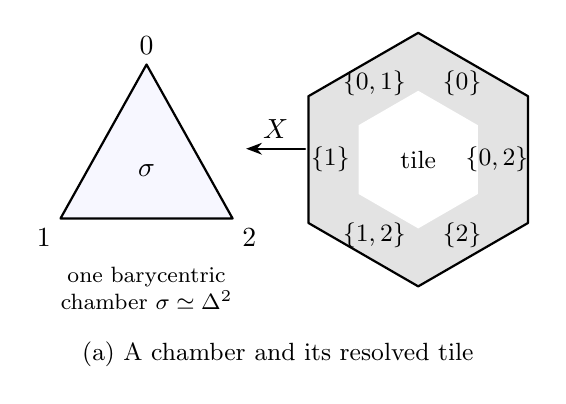
\begin{tikzpicture}[scale=1.15, line cap=round, line join=round]
  \coordinate (v0) at (-2,1.05);
  \coordinate (v1) at (-2.95,-0.65);
  \coordinate (v2) at (-1.05,-0.65);
  \draw[thick,fill=blue!3] (v0)--(v1)--(v2)--cycle;
  \node[above] at (v0) {\(0\)};
  \node[below left] at (v1) {\(1\)};
  \node[below right] at (v2) {\(2\)};
  \node at (-2,-0.12) {\(\sigma\)};
  \node[font=\footnotesize,align=center] at (-2,-1.42)
    {one barycentric\\chamber \(\sigma\simeq\Delta^2\)};
  \draw[-{Stealth[length=2mm]},thick] (-0.25,0.12)--(-0.90,0.12)
    node[midway,above] {\(X\)};
  \begin{scope}[shift={(1,0)}]
    \path[fill=gray!22,draw=black,thick]
      (30:1.40)--(90:1.40)--(150:1.40)--(210:1.40)--
      (270:1.40)--(330:1.40)--cycle;
    \path[fill=white,draw=none]
      (30:0.76)--(90:0.76)--(150:0.76)--(210:0.76)--
      (270:0.76)--(330:0.76)--cycle;
    \node[font=\small] at (60:0.97) {\(\{0\}\)};
    \node[font=\small] at (120:0.97) {\(\{0,1\}\)};
    \node[font=\small] at (180:0.97) {\(\{1\}\)};
    \node[font=\small] at (240:0.97) {\(\{1,2\}\)};
    \node[font=\small] at (300:0.97) {\(\{2\}\)};
    \node[font=\small] at (0:0.87) {\(\{0,2\}\)};
    \node[font=\small] at (0,0) {tile};
  \end{scope}
  \node[font=\small,align=center] at (-0.55,-2.15)
    {(a) A chamber and its resolved tile};
\end{tikzpicture}
\end{minipage}
\hfill
\begin{minipage}[t]{0.43\textwidth}
\centering
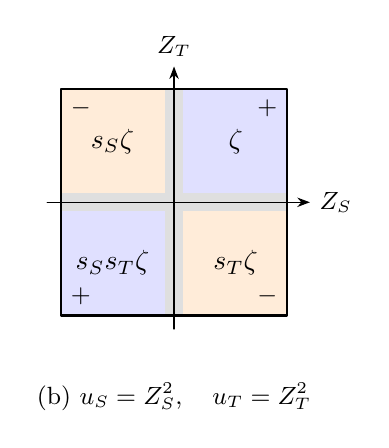
\begin{tikzpicture}[scale=1.15, line cap=round, line join=round]
  \fill[blue!12] (0,0) rectangle (1.25,1.25);
  \fill[orange!15] (-1.25,0) rectangle (0,1.25);
  \fill[orange!15] (0,-1.25) rectangle (1.25,0);
  \fill[blue!12] (-1.25,-1.25) rectangle (0,0);
  \fill[gray!25] (-0.10,-1.25) rectangle (0.10,1.25);
  \fill[gray!25] (-1.25,-0.10) rectangle (1.25,0.10);
  \draw[thick] (-1.25,-1.25) rectangle (1.25,1.25);
  \draw[-{Stealth[length=1.6mm]}] (-1.4,0)--(1.5,0)
    node[right,font=\small] {\(Z_S\)};
  \draw[-{Stealth[length=1.6mm]}] (0,-1.4)--(0,1.5)
    node[above,font=\small] {\(Z_T\)};
  \node at (0.68,0.67) {\(\zeta\)};
  \node at (-0.68,0.67) {\(s_S\zeta\)};
  \node at (0.68,-0.67) {\(s_T\zeta\)};
  \node at (-0.68,-0.67) {\(s_Ss_T\zeta\)};
  \node[font=\small] at (1.03,1.04) {\(+\)};
  \node[font=\small] at (-1.03,1.04) {\(-\)};
  \node[font=\small] at (1.03,-1.04) {\(-\)};
  \node[font=\small] at (-1.03,-1.04) {\(+\)};
  \node[font=\small,align=center] at (0,-2.15)
    {(b) \(u_S=Z_S^2,\quad u_T=Z_T^2\)};
\end{tikzpicture}
\end{minipage}
\caption{The reflected resolution in dimension two, following
Gaifullin's permutohedral construction \cite{Gaifullin2008}. In (a), one
barycentric chamber \(\sigma\simeq\Delta^2\) is paired with its resolved
tile. The six facets are indexed by the nonempty proper subsets of
\(\{0,1,2\}\); adjacent labels are nested. The map \(X\) sends the tile
interior diffeomorphically to the chamber interior. In (b), at a corner
with labels \(S\subset T\), a full state \(\zeta=(\sigma,p,t)\) and its three reflected states occupy the four
quadrants of signed coordinates. The commutation
\(s_Ss_T=s_Ts_S\) and the independent bit toggles give four distinct
quadrants of one smooth chart. The displayed signs compare each chamber
sign with that of \(\zeta\): blue agrees and orange is opposite. The gray collar
and strips represent the same seam schematically; their widths are
illustrative, and \(X\) is not affine.}
\label{fig:resolution}
\end{minipage}
\par\medskip


We verify that these are ordinary smooth charts.  On an overlap of two permutations,
a cut \(S_j\) which is not a cut of the other permutation has
\(u_j\geq4^{-2m}\).  To see this, choose a pair of indices on opposite
sides of that cut whose order is inverted in the other permutation.
Their ratio in the first ordering is at most \(4^m u_j\); its inverse
in the second ordering is at most \(4^m\).  The asserted lower bound
follows.  At a cut common to both permutations, the ratio for the
second chart is the first ratio at that cut multiplied by a product
of ratios within the blocks between common cuts.  Those within-block
ratios and their required reciprocals are bounded away from zero on
the overlap.  After taking square roots, the transition at a common
cut is consequently its signed coordinate times a smooth nonvanishing
factor.  All other transition coordinates are smooth monomials with
denominators bounded away from zero.

The sign in this transition is fixed on each region with fixed signs
at the noncommon cuts.  The remaining state relation is a product of
the common reflections, and its product is unique by their free
action on the bits.  Commutation makes this sign rule persist across
the zero coordinates.  Thus the transitions are smooth and invertible
across every corner.  A point incident to \(j\) facets has exactly the
finite star of \(2^j\) states under these reflections, and hence has
one neighborhood of this form rather than several branches.

The signed charts give smooth leaf neighborhoods.  We next check the
topological and transverse properties needed for measured integration.
The leaves are Hausdorff.  Distinct
points with distinct resolved coordinates can be separated in the
tile model.  If their resolved coordinates agree but their finite
stars differ, choose neighborhoods in these two stars avoiding all
nonincident facets; no further identification then joins them.
Each leaf has at most countably many states reachable by the finitely
many moves and at most countably many charts, so it is second countable.
The total space is standard Borel: the quotient of the state--tile
space identifies finite classes at each tile point, for which Borel
representatives can be selected by a fixed enumeration.  More
explicitly, charts can be indexed by the starting chamber, its bit
array, and the flag, with the pairing arrays as transversal parameters.
The bits determine the crossings at nonzero signed coordinates; the
moves can then be inverted to recover the pairing array.  With the
zero convention above this makes the chart maps injective.  Changes
of transversal are the measure-preserving moves on countably many
Borel overlap pieces.  A plaque meets only elementarily many plaques
in this atlas: for each second flag only the states in the two finite
flag reflection groups can occur.  These observations give precisely
the measured flow-box properties of Theorem~\ref{thm:degree}.

The chamber signs orient the leaves.  In a flag chart the Jacobian
sign from positive ratio coordinates to oriented barycentric
coordinates depends only on the permutation.  Changing one signed
coordinate from positive to negative changes the Jacobian sign of
\(u_j=Z_j^2\) once, while the move changes the chamber sign once.
The induced orientation is therefore the same across each facet.
The transverse measures here are nonnegative; the signs enter only
through this orientation in integrals of forms.  The value of
\(\omega\) is constant along each tile leaf, and translation by
\(\Gamma\) reindexes the states and preserves these measures.

\medskip\noindent\emph{The map and the local current.}
Recover the raw \(x_i\) from \eqref{eq:transfer-ratios} by normalizing
the successive products \(1,u_1,u_1u_2,\ldots,u_1\cdots u_m\).
If \(v_{\sigma,i}\) are the vertices of the indicated chamber in its
flat chart, map its tile by
\begin{equation}\label{eq:transfer-tile-map}
 X=\sum_{i=0}^m b_i v_{\sigma,i},\qquad
 b_i=\frac{\exp(-1/x_i)}{\sum_l\exp(-1/x_l)},
\end{equation}
where \(\exp(-1/x_i)\) is extended by zero at \(x_i=0\).  On a facet
with label \(S\), all coefficients outside \(S\) vanish to infinite
order in its signed coordinate.  The vertices in \(S\) are the same
on the paired chambers, and their coefficients are smooth functions
of the squares of the signed coordinates.  Thus \(X\) is smooth
through the gluing.  Its denominator is at least \(e^{-(m+1)}\), since
some \(x_i\geq1/(m+1)\), which also gives elementary upper derivative
bounds in the tile charts.

On the positive simplex the map \(x\mapsto b\) is a diffeomorphism.
Given positive \(b_i\) of sum one, its inverse is obtained from the
unique \(t\in(0,1/\max_i b_i)\) satisfying
\[
                    \sum_i\frac1{-\log(tb_i)}=1;
\]
the left side increases smoothly from zero to infinity.  The inverse
function theorem also gives the smooth inverse.  This diffeomorphism
preserves orientation.  Indeed it extends to the closed simplex
preserving every face, and the linear homotopy to the identity has
the same property, so its relative topological degree is \(+1\).
It follows that the tile interior maps diffeomorphically, with sign
\(\varepsilon_\sigma\), onto the interior of its chamber.  Each
chamber's state probability integrates to one and the tile boundaries
have leafwise measure zero.  Fubini and change of variables therefore
give, for every compactly supported smooth \(m\)-form \(\alpha\),
\[
       \int_{\mathcal A}X^*\alpha
          =\sum_\sigma\varepsilon_\sigma\int_\sigma\alpha.
\]
This proves \eqref{eq:transfer-push}.  To obtain the local identity,
define \(\mathcal A_{\rm orig}\) as the image in
\(X^{-1}(\mathcal T_\delta)\) of tile points belonging to original
chambers.  At an interior point this subset is leaf-open.  At a lower
face, the incidence argument preceding the lemma shows that every state
in its finite reflection star is on the same side.  A neighborhood in
that star can be chosen to keep its image in the strict tube and to
avoid nonincident facets, so it stays on that side.  This proves
leaf-openness and makes the definition unambiguous at glued points;
the finite indexed charts also make it Borel.  Applying the same
change-of-variables calculation only to original tile interiors, for
a form supported in \(\mathcal T_\delta\), gives
\eqref{eq:transfer-local-push}: each original cube is counted with
its coefficient \(D_0u'_C\), and each chamber's state fiber has mass one.

\medskip\noindent\emph{The metric and upper density.}
The signed charts admit a background metric \(k_0\) with elementary
bounds for its coefficients, inverse, and every fixed number of
derivatives in buffered charts.  To construct it, take smooth product
cutoffs supported in the signed boxes \((-2,2)^m\) and equal to one
on \([-1,1]^m\), and average their Euclidean chart metrics with the
normalized cutoff weights.  The smaller boxes cover, by sorted flags.
The overlap bound above bounds the number of terms per plaque.  The
transition formulas and their inverses are products of at most
\(O(m)\) factors, and every required reciprocal at a noncommon cut
is at most \(4^{O(m)}\).  Their fixed-order derivatives consequently
have elementary bounds.  These facts give the claimed bounds for the
average and its inverse, and make the construction Borel and
equivariant.  The same transition and product estimates, applied to
\eqref{eq:transfer-tile-map}, give an elementary upper bound for
\(dX\) and its fixed-order derivatives before any choice of
\(\lambda\).  The affine simplexes have diameter at most \(r\sqrt m\).

Put \(\Theta=\prod_i x_i\).  Choose a smooth \(j=j(\Theta)\) equal
to one for \(\Theta\leq\gamma_0\), zero for
\(\Theta\geq2\gamma_0\), and between zero and one elsewhere, with
the rescaled smooth cutoff estimates.  It is smooth in the signed
charts and the same on both sides of every facet.  Set
\begin{equation}\label{eq:transfer-resolution-metric}
                  k=X^*k_{\rm flat}+j^2 k_0,
       \qquad \text{seam}=\{\Theta\leq2\gamma_0\}.
\end{equation}
We call the complement of this closed seam the straight part.
The metric is positive definite near the tile boundary because \(j=1\) there.  Where
\(j<1\), one has \(\Theta>\gamma_0\), hence \(x_i\geq\gamma_0\) for
every \(i\), and \(X\) is an immersion.  The formula proves
\(\|dX\|_k\leq1\) and equality of metrics off the seam.

The upper density bound requires no inverse estimates.  As quadratic forms,
\(k\leq X^*k_{\rm flat}+k_0\), so its volume density in every sorted
box is bounded by the upper bounds for \(dX,k_0\) already chosen.
Call a common elementary bound \(H_0(q)\).  In a sorted box
\(|Z_j|\leq1\).  If all \(|Z_j|>\lambda\), normalization of the
successive products gives
\[
       \Theta\geq(m+1)^{-(m+1)}
                    \lambda^{2(1+2+\cdots+m)}
              =(m+1)^{-(m+1)}\lambda^{m(m+1)}.
\]
Condition \eqref{eq:transfer-gamma} shows that the seam lies in the
stated union of slabs.  Its coordinate volume in such a box is at
most an elementary factor times \(\lambda\).  The bound \(H_0(q)\)
was fixed before this factor was made small.

The remaining metric estimates may depend on \(\gamma_0\).  On the part
with \(j<1\), all positive ratios are bounded below by powers of
\(\gamma_0\), so the product formulas control the inverse from raw
barycentric to signed coordinates.  The normalized weights in
\eqref{eq:transfer-tile-map} obey
\(b_i\geq e^{-1/\gamma_0}/(m+1)\).  On a tangent vector
\(w=(w_i)\), \(\sum_i w_i=0\), their derivative is
\[
             db_i(w)=b_i\left(\frac{w_i}{x_i^2}
                   -\sum_l b_l\frac{w_l}{x_l^2}\right).
\]
These differences control \(w\): if their common subtracted mean is
\(a\), the relation \(\sum_iw_i=0\) expresses \(a\) as a weighted
average, with weights \(x_i^2\), of the negatives of those differences.
Thus \(|w|\) is bounded by a polynomial in \(m\) times
\(e^{1/\gamma_0}\max_i|db_i(w)|\).  Finally, the affine map from the
barycentric simplex to a simplex in a subdivided cube has elementary
inverse bounds.  Its matrix has \(r\)-scaled rational entries with
bounded denominators, and its nonzero determinant and cofactors give
this by minors.  These estimates control the inverse metric where
\(j<1\); where \(j=1\), \(k_0\) already supplies that control.
Differentiating the formula for \(k\) a fixed number of times now gives
elementary bounds, including the curvature bound, when
\(\gamma_0^{-1}\) is elementary.

\medskip\noindent\emph{Frame interpolation.}
The comparison needs a constant frame ordering tangent and normal axes
on each straight tile, a frame that glues smoothly near facets, and a homotopy to the
identity for the degree calculation.  Choose a Borel skew-symmetric logarithm
\(A_\sigma\) of each \(O_\sigma\) with operator norm at most \(\pi\).
Such a choice follows by decomposing an orthogonal rotation into its
two-dimensional angle blocks with principal angles and, on its
\(-1\)-eigenspace, pairing a Borel choice of orthonormal basis; the
even dimension there follows from determinant one.  Define on that
tile
\[
                   \mathcal R=\exp((1-j)A_\sigma).
\]
It is the identity in a neighborhood of each facet and thus glues
smoothly despite the change of \(\sigma\).  It equals \(O_\sigma\)
where \(j=0\), and replacing \(1-j\) by \(t(1-j)\), \(0\leq t\leq1\),
gives the asserted homotopy.  The cutoff and metric inverse estimates
give the derivative bounds.  The choices can be made on the indexed
chamber data, so they are Borel and equivariant as asserted.
\end{proof}

For our use, choose \(O_\sigma\) to take \(z\)-increments to rotated
grid increments, putting the \(m\) axes tangent to the dual cube first
and the \(n\) complementary axes last.  Use a signed permutation if
needed to have determinant one.  Thus \(O_\sigma=Q_\sigma V\) for a
signed permutation \(Q_\sigma\in SO(q)\) with this order.  Signs will
not affect any row norm or any cubical test.

\subsection{The comparison map and its degree}

The parameter selection below fixes \(\lambda(q)\) and \(\gamma_0(q)\)
deterministically.  For those choices the bounds in
Lemma~\ref{lem:transfer-resolution} give fixed elementary numerical
envelopes \(K_R(q)\) and \(K_{\rm scal}(q)\) such that
\[
 \|d\mathcal R\|_{\infty,k}\leq K_R(q),\qquad
                    (-\Scal_k)_+\leq K_{\rm scal}(q)
\]
for every allowed diagram and every \(V,s,\omega\), rounding parameter,
and state.  These envelopes come from the uniform chart derivative
bounds and do not use \(C_{\rm ent}\).  Fix the single number
\begin{equation}\label{eq:transfer-tau}
 \tau=\tau(q)=
 \frac{1}{300\sqrt q\max\{r^{-1},\delta^{-1},1+K_R(q)\}}.
\end{equation}
It has an elementary reciprocal and is common to all those parameters.
In particular
\(3\tau\sqrt q\leq\min\{r/100,\delta/100,(1+K_R(q))^{-1}\}\).

Fix \(V,s\) and the rounding parameter for the moment.  Take the
product of \(\widetilde M\) and the tile family \(\mathcal A\) over
their shared \(\omega\), and divide by the diagonal \(\Gamma\)-action.
Orient the product with the \(\widetilde M\) directions first and the
\(\mathcal A\) directions second.  The resulting measured leaves have
dimension \(n+m=q\).  Using the leaf-open set
\(\mathcal A_{\rm orig}\) from Lemma~\ref{lem:transfer-resolution},
work only on the open set of pairs \((x,a)\) with
\(a\in\mathcal A_{\rm orig}\) for which \(X(a)\) is in the lift of the ball chart of
\(F(x)\), at distance less than \(\delta/4\).  Define there
\begin{equation}\label{eq:transfer-comparison}
                   G(x,a)=\mathcal R(a)(z_F(x)-z_{X(a)}).
\end{equation}
Here \(z_{X(a)}=z\circ X(a)\).  The requirement on the lifts is part of
the domain; coincident color coordinates on incompatible sheets are
never compared.  The map is invariant under the diagonal action.

Use the band \(\{|G|_\infty<3\tau\}\) in that open domain, and put
\(b_q=\tau(1+3/(4q))\), the inner width in Theorem~\ref{thm:degree}
when \(d=q\).  Let \(\mathcal D\) be its measured degree.

\begin{lemma}[Comparison degree]\label{lem:transfer-degree}
The band in \eqref{eq:transfer-comparison} satisfies the chart and
integration control assumptions of Theorem~\ref{thm:degree}, for each
fixed instance, the product metric \(h+L^2k\) with any fixed \(L>0\),
and the pullback of the entropy weight \(\phi\).  Its degree is Borel
in the auxiliary parameters and satisfies
\begin{equation}\label{eq:transfer-degree}
                         \E_{\rm rd}\mathcal D=D_0I
\end{equation}
for every fixed \(V,s\).
\end{lemma}

\begin{proof}
The local pushforward \eqref{eq:transfer-local-push} will express the
degree using a smoothed form of \(Z_{\rm rd}\).  Its primal-cell periods
are the integer coefficients \(D_0u'_C\).  Their expectations match the periods of
\(D_0\eta\); a compatible piecewise cubical primitive and mollification
then give the same measured pairing with \(F\).  We first verify the
band control that makes these integrations valid.

\emph{The controlled comparison band.}
Before taking the quotient, the product flow boxes use the entropy
transversal \(\omega\) and the
state transversals of \(\mathcal A\).  Variation along the tile keeps
\(\omega\) constant.  These transversals carry the invariant measures
constructed above.  A group element that stabilizes a product leaf
acts freely and properly because it acts so on the \(\widetilde M\)
factor.  Hence the quotient leaves are ordinary oriented Hausdorff
second countable manifolds.  The actions reindex labels and states,
leave the color and flag coordinates unchanged, and preserve the
transverse measures and orientations.

For an inner closed comparison cube there is a uniform margin from
the boundary of the allowed sheet domain.  Indeed \(\mathcal R\) is
orthogonal and \eqref{eq:transfer-tau} gives
\(|z_F-z_X|_2\leq3\tau\sqrt q\ll\delta/4\).  The large witness
color at \(F\) remains present with a uniform small buffer.  In a
flat ball chart a lifted path whose projected coordinates stay in
the ball stays in that same lift, by uniqueness of lifts for a local
diffeomorphism.  The nearby points therefore remain in coherent
sheet charts.  Facets that lead to the mirror are outside this region.
The available smooth bounds for the instance give fixed buffered
coordinate charts for all the data in these regions.

To check the finiteness condition on those charts, choose lifts of a
finite buffered atlas on \(M\).  On their compact closures \(F\) uses
only uniformly finitely many possible labels, by the lifted support
bounds in Theorem~\ref{thm:entropy}.  Any nearby cell lift has its
anchor in a closed one-neighborhood of one of these labels.  The
numbers of projected grid indices, chamber subdivisions, and copies
there are bounded as above.  Thus only finitely many chamber indices
are needed over each such base chart, uniformly for the instance.
Their state probabilities have total mass one per chamber, and the
sum of transverse measures of this covering is finite.  Plaque
overlaps are bounded by the tile overlap bound and the bounded
overlap of the base atlas.  In the quotient only finitely many deck
changes meet two of these buffered base charts.  Subdividing their
inner boxes and, when necessary, restricting to Borel transverse sets
gives the flow boxes stipulated in Theorem~\ref{thm:degree}.  All
metric and data bounds in this verification may depend on the
instance.  It also justifies Fubini and measured Stokes for the
integrations that follow.

\medskip\noindent\emph{The local convolution form.}
Choose a smooth unit-integral top form \(\beta\) on \(\mathbb R^q\)
supported in a Euclidean ball about zero of radius less than
\(\min\{\tau,r/10\}\).  In calculating the degree using \(\beta\),
homotope \(\mathcal R\) to the identity as in
Lemma~\ref{lem:transfer-resolution}.  All maps in this homotopy are
orthogonal on the difference variable.  Their pullbacks of \(\beta\)
are thus supported where the difference has this same small norm,
strictly inside both the sheet domain and the original band.  Measured
Stokes for this supported homotopy shows that it does not change the
degree.

After removing the rotation, fiber integration of
\((z,w)\mapsto z-w\) against \(\beta\) and the original current
\(Z_{\rm rd}\) gives a smooth \(n\)-form \(\alpha_{\rm rd}\) near \(K\).
More explicitly, in a flat chart put \(\mathsf d(z,w)=z-w\).  Integrate
\(\mathsf d^*\beta\) along each compatible \(C^\#\) in the second
variable, multiply by \(D_0u'_C\), and sum.  The sum is locally finite
and uses the original side.  By the local identity
\eqref{eq:transfer-local-push}, Fubini, and change of variables on tile
interiors, the degree is
\begin{equation}\label{eq:transfer-convolution-degree}
                       \mathcal D=\int_{\mathcal M}F^*\alpha_{\rm rd}.
\end{equation}
Boundary cancellation of the dual cubes shows that
\(d\alpha_{\rm rd}=0\) on, for example, the tube of radius
\(\delta/8\) around \(K\).  To verify this directly, apply fiber
Stokes to each cube.  Its boundary terms only involve facets within
the support distance of the point \(z\); these lie in the balanced
tube and cancel with their paired incidence signs.

For every primal \(n\)-cell sufficiently near \(K\) in the same
sheet,
\begin{equation}\label{eq:transfer-convolution-cells}
                         \int_C\alpha_{\rm rd}=D_0u'_C.
\end{equation}
Indeed a primal \(n\)-cell and a complementary dual \(m\)-cell of
this grid meet only when their indices match, and then at their common
center.  If their axis sets differ, a coordinate fixed for both is a
grid vertex for the primal cell and a half-step center for the dual
cell, so their difference in that coordinate is at least \(r/2\).
If their axis sets agree but their grid indices differ, a differing
coordinate gives the same separation.  Such pairs cannot meet the
support of \(\beta\).  For the matching pair, the difference map
from \(C\times C^\#\) contains the support ball in its image with
multiplicity one.  Our fiber integration convention is
\(\int_C\int_{C^\#}\mathsf d^*\beta=
\int_{C\times C^\#}\mathsf d^*\beta\) with the base-first product
orientation.  The differential of \(\mathsf d(z,w)=z-w\) sends this
ordered frame to the primal basis followed by the negative dual basis,
so its orientation is positive by our choice of the dual orientation.
Its integral is therefore
one, proving \eqref{eq:transfer-convolution-cells}.  The small support
and the chart buffers ensure that only the indicated lifts contribute.

\medskip\noindent\emph{The detector pairing.}
Set \(\alpha=\E_{\rm rd}\alpha_{\rm rd}-D_0\eta\).  It is a smooth
closed form on that tube, and \eqref{eq:transfer-rounding},
\eqref{eq:transfer-cell-value}, and
\eqref{eq:transfer-convolution-cells} give \(\int_C\alpha=0\) on all
the primal \(n\)-cells there.  We explain why its measured pairing
with \(F\) vanishes, including when \(F\) meets grid faces.

Use all lifted full \(q\)-cells needed to cover the tube of radius
\(\delta/32\) around \(K\).  Taking \(r\sqrt q\) sufficiently small
as above, these cells lie in the tube of radius \(\delta/8\), all
their \(n\)-faces are selected, and their shared faces fit in
coherent sheet charts.  On one grid interval \([a,a+r]\), project a
function to its linear interpolation between the endpoints and
project a one-form \(f(t)dt\) to the constant one-form with the same
integral.  The homotopy for a one-form is the function
\[
       \mathsf h(f(t)dt)(t)=\int_a^t
              \left(f(v)-r^{-1}\int_a^{a+r}f(s)\,ds\right)dv,
\]
which vanishes at both endpoints; the homotopy on functions is zero.
Direct differentiation gives \(\mathrm{id}-\mathsf P
=d\mathsf h+\mathsf h d\).  Apply these operations one coordinate
at a time, with the ordinary exterior differential signs.  The
tensor-product homotopy still commutes with tangential restriction
to a face, since the one-dimensional primitive vanishes at the
endpoints.  The full projection of an \(n\)-form has, for each
axis set, coefficients obtained by integrating on its \(n\)-faces
and interpolating linearly in the remaining axes.  Hence the full
projection of \(\alpha\) is zero.  Since \(d\alpha=0\), the
homotopy supplies a primitive on each full cube, and its tangential
restrictions agree on shared faces.

This piecewise primitive has bounded coefficients for the instance
and is also a weak primitive on the tube: in distributional Stokes
the terms on each shared face cancel by agreement of its tangential
restrictions.  On a smaller tube mollify it in the flat coordinates.
This can be done with the same small Euclidean convolution in every
chart: the buffered sheets give a unique lift of the convolution ball,
and on overlaps the piecewise primitive and flat coordinates agree.
Its smooth exterior derivatives are the mollifications of the smooth
form \(\alpha\), and converge to \(\alpha\) there.  The construction
is Borel and equivariant and has bounded coefficients for the instance.
Measured Stokes applied to the pullback of each smooth primitive gives
zero; convergence and the uniform chart bounds give
\(\int_{\mathcal M}F^*\alpha=0\).  All expectations and integrals
above are measurable by their locally finite chart formulas, and
their absolute bounds for the instance justify their interchange.
Using \eqref{eq:transfer-form} in
\eqref{eq:transfer-convolution-degree} now proves
\eqref{eq:transfer-degree}.
\end{proof}

\subsection{The two comparison lengths and the final average}

We finish by estimating these degrees.  We will see separately how
the straight part uses the dimension-only Hilbert norm of \(\eta\)
and how the small coordinate volume of the seam pays for its rougher
bound.

\begin{proof}[Proof of Theorem~\ref{thm:scalar-volume}]
The case \(\|M\|=0\) is immediate.  Otherwise we first prove the
conditional target for the data above, choosing \(\Psi_n\) from the
requirements on \(E\) derived below, and then apply it to the entropy
output.  Choose a positive constant \(b_*\), depending only on \(n\),
whose smallness will be fixed in the estimate below, and put
\begin{equation}\label{eq:transfer-lengths}
       L_T=b_*\sqrt E,\qquad L_N=b_*\sqrt{qE},\qquad
                    h_{\rm tot}=h+L_T^2k.
\end{equation}
Once the degree hypotheses are verified, its length denominator, the
product volume, and the entropy contribution will combine as
\begin{equation}\label{eq:transfer-prefactor}
 \frac{L_T^mE^{n/2}}{L_T^mL_N^n}\,e^{-W}dV_h
                         =b_*^{-n}q^{-n/2}\rho.
\end{equation}
This is the cancellation of the tangent volume and all powers of
\(E\).  The estimates below justify the degree application and bound
the straight angular sum by a dimensional multiple of \(q^{n/2}\),
while the collar volume controls the seam.

Use the weight \(\phi\), constant in the tile directions.  The
product scalar formula and the definition of \(\wscal\) give
\(\wscal(h_{\rm tot},\phi)=\wscal(h,\phi)+L_T^{-2}\Scal_k\).
By the definition of \(K_{\rm scal}(q)\), the lower bound
\(E\geq b_*^{-2}K_{\rm scal}(q)\) ensures
\(L_T^{-2}\Scal_k\geq-1\).  By \eqref{eq:transfer-entropy},
\begin{equation}\label{eq:transfer-total-scalar}
 \wscal(h_{\rm tot},\phi)\geq-C_{\rm ent}-1+2W-n\log E+E\mathfrak e.
\end{equation}

Assign \(L_i=L_T\) to the first \(m\) comparison rows and
\(L_i=L_N\) to the last \(n\) rows.  On the band, the derivative in
tile directions of each row of \(G\), measured with \(k\), has norm
at most two.  The \(dX\) term has norm at most one, and the
\(d\mathcal R\) term has norm at most
\(3\tau\sqrt q\|d\mathcal R\|_k\leq1\) by
\eqref{eq:transfer-tau}.  The horizontal derivative is a row of a
rotation of \(dz_F\).  It follows that
\[
 L_i|dG_i|_{h_{\rm tot}}
       \leq C_n\bigl(\sqrt q+\sqrt{qE}\,E^{-1/100}\bigr).
\]
Take \(B\) to be this upper bound increased by two.  Then
\(L_i|dG_i|\leq B-1=B-q/q\).  The horizon condition of
Theorem~\ref{thm:degree} holds after an elementary increase of \(E\):
it suffices to test the smallest length \(L_T\), and, for \(E\geq1\),
\[
       \frac{C(1+B)^{2/3}}{L_T}
          \leq c_{{\rm hor},n}q^{1/3}E^{-13/75}
          <\frac{\tau}{10q}.
\]
Here \(c_{{\rm hor},n}\) depends only on the absolute horizon constant
and the dimensional choice of \(b_*\), and
\(13/75=1/2-(2/3)(1/2-1/100)>0\).  Thus the displayed strict horizon
inequality follows if
\(E\geq(20c_{{\rm hor},n}q^{4/3}/\tau)^{75/13}\).
We may therefore apply Theorem~\ref{thm:degree}
with \(d=q\).

Write \(H_i=2(L_i|dG_i|-1)_+\), as in that theorem.  At a straight
point in a tile, let \(\mathcal I\) be the \(n\)-set of grid axes
normal to its dual cube.  Put \(A_i=(Vdz_F)_i\), with covector norms
measured by \(h\), and define
\begin{equation}\label{eq:transfer-U}
       U_{\mathcal I}^2=
        \frac q{\mathfrak e}\sum_{i\in\mathcal I}|A_i|_h^2
        \quad\text{if }\mathfrak e>0,
        \qquad U_{\mathcal I}=0\quad\text{if }\mathfrak e=0.
\end{equation}
Here \(\sum_i|A_i|^2=\mathfrak e\).  At a straight point
\(k=X^*k_{\rm flat}\) and \(\mathcal R=Q_\sigma V\) is constant.
For a tangent comparison row corresponding to axis \(i\), the squared
row norm is exactly \(L_T^{-2}+|A_i|^2\).  Thus
\[
  \sum_{\rm tangent}H_i
      \leq L_T^2\mathfrak e=b_*^2E\mathfrak e,
\]
by \(2(\sqrt{1+t}-1)\leq t\).  Normal rows have no tile derivative,
so Cauchy--Schwarz gives
\[
  \sum_{\rm normal}H_i
    \leq2L_N\sum_{i\in\mathcal I}|A_i|
    \leq2b_*\sqrt n\sqrt{E\mathfrak e}\,U_{\mathcal I}.
\]
Completing the square in \(\sqrt{E\mathfrak e}\), for \(b_*<1\),
shows that
\begin{equation}\label{eq:transfer-straight-penalty}
       \frac{\sum_iH_i-E\mathfrak e}{2}
          \leq c_n U_{\mathcal I}^2,
       \qquad c_n=\frac{n b_*^2}{2(1-b_*^2)}.
\end{equation}

Choose \(b_*\) sufficiently small that
\begin{equation}\label{eq:transfer-sphere}
                  \E_V\exp(2c_nU_{\mathcal I}^2)\leq C_n
\end{equation}
for every fixed horizontal differential and every fixed
\(\mathcal I\).  Here is a direct verification of this choice.  If
\(u\) is one coordinate of a uniform point on \(S^{q-1}\), its sphere
moments satisfy
\[
 \E(q u^2)^j
   =\frac{q^j(1\cdot3\cdots(2j-1))}{q(q+2)\cdots(q+2j-2)}
   \leq2^j j!.
\]
Consequently \(\E e^{tqu^2}\leq(1-2t)^{-1}\) for \(0\leq t<1/2\).
The singular-value decomposition of \(dz_F\) expresses each
\(q|A_i|^2/\mathfrak e\) as a convex combination of such random
variables, with its singular-value weights.  Jensen's inequality
gives the same exponential bound for that convex combination.
Another application of Jensen to the sum of the \(n\) rows in
\eqref{eq:transfer-U} bounds its exponential moment by
\((1-2nt)^{-1}\).  Choosing, for instance, \(2nc_n<1/4\) proves
\eqref{eq:transfer-sphere}.  No independence of the rows of \(V\)
is used.

At a seam point the uniform tile row bound gives a rougher estimate
which is still independent of the instance.  By the triangle inequality
for each row, \((a-1)_+\leq a\), and Cauchy--Schwarz on the horizontal
rows,
\[
 \sum_iH_i\leq 2L_N\sqrt{q\mathfrak e}
                   +4q L_N/L_T
       \leq2b_*q\sqrt{E\mathfrak e}+4q^{3/2}.
\]
Completing the square once more gives
\begin{equation}\label{eq:transfer-seam-penalty}
 \frac{\sum_iH_i-E\mathfrak e}{2}\leq c_{{\rm seam},n}q^2,
                 \qquad c_{{\rm seam},n}=2+\frac{b_*^2}{2}.
\end{equation}

Apply the degree inequality, then use
\eqref{eq:transfer-total-scalar}.  Its loss is \(\exp(Cq/q)\), an
absolute constant.  The product volume form is
\(dV_{h_{\rm tot}}=L_T^m dV_h\,dV_k\), so the measure factor is
exactly \eqref{eq:transfer-prefactor}.  Together with
\eqref{eq:transfer-degree} and \(|\E\mathcal D|\leq\E|\mathcal D|\),
this gives the following inequality, with
\(C_{\rm out}=\exp(C_{\rm deg}+(C_{\rm ent}+1)/2)b_*^{-n}\), where
\(C_{\rm deg}\) is the absolute exponent in Theorem~\ref{thm:degree}:
\begin{equation}\label{eq:transfer-average}
 \begin{split}
 D_0I(2\tau)^q\leq C_{\rm out}q^{-n/2}
  \int_{\mathcal M}\rho\,
   \E_{V,s,\rm rd}
     \int_{\{a:\ |G(x,a)|_\infty<b_q\}}
                       \mathcal B(x,a)\,dV_k(a),
 \end{split}
\end{equation}
where the fiber integral includes its state transversals and only the
compatible original-side band, and
\[
 \mathcal B(x,a)=
 \begin{cases}
    \exp(c_nU_{\mathcal I}^2),&a\text{ straight over axes }\mathcal I,\\
    \exp(c_{{\rm seam},n}q^2),&a\text{ in the seam}.
 \end{cases}
\]
The entropy constant enters only through this final prefactor, not the
geometric bounds used below.  The length and volume prefactor has no
exponential loss in \(m\); the seam exponential will be absorbed by
the choice of \(\lambda\).

Fix \(x,\omega\), and put \(y=F(x)\).  At a coupled pair in
\eqref{eq:transfer-average}, a fixed projected grid index has at most
one possible cell lift in the ball chart of \(y\).  Its full primal
and dual cells fit in that chart by \eqref{eq:transfer-tau} and the
buffers, and the lift there is unique.  Moreover each point of its
primal cell is within \(10r\sqrt q\) of \(y\): the dual point is
within \(b_q\sqrt q\) of \(y\), and the dual and primal extents are
at most \(r\sqrt m/2\) and \(r\sqrt n/2\).  The variation choice
for \(r\) and the rounding error now give the copy-count estimate
\begin{equation}\label{eq:transfer-copies}
       D_0|u'_C|\leq D_0r^n
                        \bigl(|\eta_{\mathcal I}(y)|+2q^{-n}\bigr),
\end{equation}
where the component is in the \(V\)-rotated frame.

On a straight tile the \(k\)-volume is exactly the flat volume of
its image in the chamber.  The signed permutation in \(G\) does not
change its cube test, which is
\(|\widehat z_y-\widehat z_X|_\infty<b_q\).  Summing the chamber
pieces in a copy is thus bounded by the \(m\)-area of its whole dual
cube inside that test; the state probabilities for each chamber
integrate to one.  For a fixed axis set \(\mathcal I\), summing over
all projected centers and averaging the shift gives exactly
\begin{equation}\label{eq:transfer-shift}
  r^{-q}\int_{\mathbb R^q}\int_{[-r/2,r/2]^m}
       \indic_{\{|\widehat z_y-c-t|_\infty<b_q\}}\,dt\,dc
                    =r^{-q}r^m(2b_q)^q.
\end{equation}
Here \(t\) is placed in the complementary axes.  This identity is
just the density \(r^{-q}\) of centers under uniform shift; extending
the sum to the full grid is an upper bound for the selected lifted
cells.

The form bound holds in every rotated frame.  Using Cauchy--Schwarz
jointly in \(V\) and the \(\binom qn\) axis sets, and then
\eqref{eq:transfer-sphere}, we obtain
\begin{equation}\label{eq:transfer-form-average}
 \begin{split}
 \E_V\sum_{|\mathcal I|=n}
   (|\eta_{\mathcal I}(y)|+2q^{-n})e^{c_nU_{\mathcal I}^2}
 &\leq
   \left(\E_V\sum_{\mathcal I}|\eta_{\mathcal I}(y)|^2\right)^{1/2}
   \left(\E_V\sum_{\mathcal I}e^{2c_nU_{\mathcal I}^2}\right)^{1/2}
       +C_nq^{-n}\binom qn\\
 &\leq C_nq^{n/2}.
 \end{split}
\end{equation}
This use of Cauchy--Schwarz allows the form components and row norms
to depend on the same rotation.  Combining
\eqref{eq:transfer-copies}--\eqref{eq:transfer-form-average}, the
straight part of the inner expectation in
\eqref{eq:transfer-average} is at most
\(C_nD_0q^{n/2}(2b_q)^q\), because \(r^{n+m-q}=1\).  Multiplying
by its prefactor \(q^{-n/2}\) bounds that part, for a fixed
dimension-only constant \(C_{{\rm str},n}\), by
\begin{equation}\label{eq:transfer-straight-average}
             C_{{\rm str},n}D_0(2\tau)^q,
\end{equation}
since \((b_q/\tau)^q=(1+3/(4q))^q\leq e^{3/4}\).

For the seam use only the consequence
\(|z_X-z_y|_2\leq b_q\sqrt q\) of the cube test.  Discard the tile
boundaries, which have leafwise measure zero.  The remaining set is
the disjoint union of tile interiors indexed by their \emph{actual}
chamber \(\sigma\) and its state arrays.  Partition each such interior
into positive sorted-coordinate pieces, for example by taking the
first sorted permutation in a fixed order.  On these pieces
\(0<Z_j\leq1\), so no signed-chart reflection changes the chamber.
The conditional state measure over each actual chamber has mass one,
and its \(k\)-density is at most the elementary \(H_0(q)\) chosen
before \(\lambda\).

Retain the compatible-sheet restriction at this point.  For a fixed
projected grid index the uniqueness proved before
\eqref{eq:transfer-copies} allows at most one compatible geometric
lift.  Apply the rough copy bound
\(D_0|u'_C|\leq C_{\eta,n}D_0r^n\) from that equation, where
\(C_{\eta,n}\) depends only on the form norm, and use the uniform
density bound.  Only after these bounds may we drop the restrictions
on available sheets, roundings, and chambers and sum over all projected
centers and chamber shapes.

For a fixed actual chamber shape, normal axis set \(\mathcal I\), and
positive sorted flag, \eqref{eq:transfer-tile-map} has rotated position
\[
 \widehat z_X=s+r\left(k+\tfrac12\indic_{\mathcal I}\right)
                       +d_{\mathcal I,\mathrm{shape},\mathrm{flag}}(Z).
\]
Here \(\indic_{\mathcal I}\) is the coordinate indicator vector of
\(\mathcal I\).
The displacement \(d\) is independent of the pairing and bit arrays,
of \(\lambda,\gamma_0\), and of the shift; it is determined by the
fixed chamber shape and the barycentric formula.  For each fixed \(Z\)
the shift integral of the rough test is consequently
\[
 \begin{split}
 \frac1{r^q}\int_{[0,r)^q}\sum_{k\in\mathbb Z^q}
  \indic_{\{|s+r(k+\frac12\indic_{\mathcal I})+d(Z)-\widehat z_y|_2
                  \leq b_q\sqrt q\}}\,ds
 &=r^{-q}\Vol_{\mathbb R^q}(B_{b_q\sqrt q})\\
 &\leq r^{-q}(4\tau\sqrt q)^q.
 \end{split}
\]
This calculation is valid despite the shift dependence of the actual
diagram, because the copy, lift, and density bounds were imposed before
the enlargement to all centers.  Tonelli's theorem applies to these
nonnegative bounds.

In each positive sorted piece the seam lies in
\(\bigcup_j\{Z_j\leq\lambda\}\), of coordinate volume at most
\(m\lambda\).  A cube has \(2^m m!\) barycentric top chambers and
at most \((m+1)!\) sorted flags per chamber.  Thus the seam part of
the inner expectation is bounded by
\begin{equation}\label{eq:transfer-seam-average}
                    C_*(q)\lambda D_0(2\tau)^q,
\end{equation}
where one may take the elementary envelope
\[
 C_*(q)=\max\left\{1,\,
 C_{\eta,n}H_0(q)\binom qn(2^m m!)(m+1)!\,m\,
 r^{n-q}(2\sqrt q)^q\exp(c_{{\rm seam},n}q^2)\right\}.
\]
Every factor here was bounded before choosing \(\lambda\).  Thus
\(C_*\) is independent of \(\lambda,\gamma_0,\tau\), of the bounds
\(K_R,K_{\rm scal}\), and of \(C_{\rm ent}\).  The powers \(\tau^q\) in the shift
count have already canceled those in \((2\tau)^q\).

The two fiber estimates now have the same normalization.  Insert
\eqref{eq:transfer-straight-average} and
\eqref{eq:transfer-seam-average} into \eqref{eq:transfer-average},
using \(q^{-n/2}\leq1\) for the seam, and cancel the positive factor
\(D_0(2\tau)^q\).  For the conditional data and parameter bounds used
so far, this gives
\begin{equation}\label{eq:transfer-before-choices}
       I\leq C_{\rm out}\bigl(C_{{\rm str},n}+C_*(q)\lambda\bigr)
                           \int_{\mathcal M}\rho.
\end{equation}

We now fix these bounds before invoking the entropy theorem.  For each
integer \(q\geq n+1\), the form derivative bound first gives a
deterministic \(r(q)\) with elementary reciprocal.  The size bound for
the universal type list, \(D_0\), incidence counts, and the bounds for
\(k_0,dX\), including \(H_0(q)\), have elementary envelopes uniform
over all permitted graphs and cocycles.  Fix \(b_*\) using
\eqref{eq:transfer-sphere}; this determines the dimensional constants
\(c_{{\rm seam},n}\) and \(c_{{\rm hor},n}\), independently of
\(C_{\rm ent}\).  The displayed formula for \(C_*(q)\) is consequently
available at this stage.  Set
\[
 \lambda(q)=\frac1{4C_*(q)},\qquad
 \gamma_0(q)=\frac14(m+1)^{-(m+1)}\lambda(q)^{m(m+1)}.
\]
These deterministic choices have elementary reciprocals and satisfy
\eqref{eq:transfer-gamma}.  The resolution estimates now give common
elementary envelopes for its fixed-order chart derivatives, hence
\(K_R(q),K_{\rm scal}(q)\), and then the common \(\tau(q)\) in
\eqref{eq:transfer-tau}.  None of these choices uses the entropy constant.

For integer \(j\geq n+1\), define
\[
 \Psi_n^\circ(j)=\max\left\{1,\ b_*^{-2}K_{\rm scal}(j),
       \left(\frac{20c_{{\rm hor},n}j^{4/3}}{\tau(j)}\right)^{75/13}
                      \right\},
\]
and define a majorant on all \(t\in[1,\infty)\) by
\[
 \Psi_n(t)=1+\max_{\substack{j\in\mathbb Z\\
                   n+1\leq j\leq\max\{n+1,\lceil t\rceil\}}}
                            \Psi_n^\circ(j).
\]
Every expression used here has an elementary upper bound; the finite
maximum is bounded by an increasing elementary envelope at
\(\max\{n+1,\lceil t\rceil\}\).  Thus \(\Psi_n\) is an elementary
majorant fixed solely from \(n\), and it dominates both the curvature
and strict horizon requirements.  Hence every conditional datum with
\(E\geq\Psi_n(q)\) satisfies all hypotheses used in
\eqref{eq:transfer-before-choices}.  Our choice
\(C_*(q)\lambda(q)=1/4\) and the definition of \(C_{\rm out}\) prove
\eqref{eq:transfer-conditional-target} with
\[
       K_n=e^{C_{\rm deg}+1/2}b_*^{-n}
                             \bigl(C_{{\rm str},n}+1/4\bigr).
\]
This closes the conditional target for all the specified data before
any entropy family is chosen.

Now apply Theorem~\ref{thm:entropy} with \(\mathcal B=\Psi_n\),
\(E_{\min}=1\), the detector root map as \(F^{\mathrm{in}}\), and the
one-point transverse space \(\Omega_0\).  The detector construction uses
finitely many compactly supported bump representatives and their deck
translates, giving the required uniform support and derivative bounds in
a lifted atlas and the equivariant compact support sets.  After pulling
the detector map to \(\Omega\) and embedding its labels equivariantly
among the output's finite copies, the measured affine probability homotopy
of Section~2 preserves \(I\); the output therefore supplies the conditional
data with \(E>\Psi_n(q)\).  Its constant
\(C_{\rm ent}=C_{\rm ent}(n,\Psi_n)\) depends only on \(n\).  Since
\(\rho\leq dV_g\) and the transverse measure over \(M\) is a
probability measure,
\[
           I\leq K_ne^{C_{\rm ent}/2}\int_{\mathcal M}\rho
             \leq K_ne^{C_{\rm ent}/2}\Vol_g(M).
\]
Finally \(I\geq\|M\|/2\), so the constant
\(C_n=2K_ne^{C_{\rm ent}/2}\) proves the theorem.
\end{proof}

\begin{proof}[Proof of Theorem~\ref{thm:main}]
Fix \(n\geq3\), and let \(C_n>0\) be the constant for the normalized
scalar-curvature estimate in Theorem~\ref{thm:scalar-volume}.
Proposition~\ref{prop:yamabe-reduction} gives
\[
              \|M\|\leq C_n\int_M(\Scal_g^-)^{n/2}\,dV_g
\]
for every metric in the theorem.  Taking \(a_n=C_n^{-1}>0\) proves
the stated integral bound.
\end{proof}

\begin{thebibliography}{99}

\bibitem{Allard1972}
W. K. Allard, \emph{On the first variation of a varifold},
Annals of Mathematics (2) \textbf{95} (1972), no. 3, 417--491.
\href{https://doi.org/10.2307/1970868}{doi:10.2307/1970868}.

\bibitem{Aubin1976}
T. Aubin, \emph{\'Equations diff\'erentielles non lin\'eaires et
probl\`eme de Yamabe concernant la courbure scalaire},
Journal de Math\'ematiques Pures et Appliqu\'ees (9) \textbf{55}
(1976), no. 3, 269--296.

\bibitem{BraunSauer2021}
S. Braun and R. Sauer, \emph{Volume and macroscopic scalar curvature},
Geometric and Functional Analysis \textbf{31} (2021), 1321--1376.
\href{https://doi.org/10.1007/s00039-021-00588-y}
{doi:10.1007/s00039-021-00588-y}.

\bibitem{ChodoshLi2024}
O. Chodosh and C. Li, \emph{Generalized soap bubbles and the topology
of manifolds with positive scalar curvature},
Annals of Mathematics (2) \textbf{199} (2024), no. 2, 707--740.
\href{https://doi.org/10.4007/annals.2024.199.2.3}
{doi:10.4007/\allowbreak annals.2024.199.2.3}.

\bibitem{Eichmair2009}
M. Eichmair, \emph{The Plateau problem for marginally outer trapped
surfaces}, Journal of Differential Geometry \textbf{83} (2009),
no. 3, 551--583.
\href{https://doi.org/10.4310/jdg/1264601035}
{doi:10.4310/jdg/1264601035}.

\bibitem{Frigerio2016}
R. Frigerio, \emph{Bounded cohomology of discrete groups},
preprint, 2016.
\href{https://arxiv.org/abs/1610.08339v2}{arXiv:1610.08339v2}.

\bibitem{Gaifullin2008}
A. A. Gaifullin, \emph{Realisation of cycles by aspherical manifolds},
Russian Mathematical Surveys \textbf{63} (2008), no. 3, 562--564.
\href{https://doi.org/10.1070/RM2008v063n03ABEH004540}
{doi:10.1070/RM2008v063n03ABEH004540};
\href{https://arxiv.org/abs/0806.3580}{arXiv:0806.3580}.

\bibitem{Gaifullin2013}
A. Gaifullin, \emph{Universal realisators for homology classes},
Geometry \& Topology \textbf{17} (2013), no. 3, 1745--1772.
\href{https://doi.org/10.2140/gt.2013.17.1745}
{doi:10.2140/gt.2013.17.1745}.

\bibitem{GilbargTrudinger}
D. Gilbarg and N. S. Trudinger,
\emph{Elliptic Partial Differential Equations of Second Order},
second edition, Classics in Mathematics, Springer, Berlin, 2001.
\href{https://doi.org/10.1007/978-3-642-61798-0}
{doi:10.1007/978-3-642-61798-0}.

\bibitem{Gromov1982}
M. Gromov, \emph{Volume and bounded cohomology},
Publications Math\'ematiques de l'IH\'ES \textbf{56} (1982), 5--99.
\href{https://www.numdam.org/item/PMIHES_1982__56__5_0/}
{Numdam: PMIHES\_1982\_\_56\_\_5\_0}.

\bibitem{Gromov1986}
M. Gromov, \emph{Large Riemannian manifolds}, in
\emph{Curvature and Topology of Riemannian Manifolds},
K. Shiohama, T. Sakai, and T. Sunada (eds.),
Lecture Notes in Mathematics \textbf{1201}, Springer, Berlin, 1986,
108--121.
\href{https://doi.org/10.1007/BFb0075649}{doi:10.1007/BFb0075649}.

\bibitem{Gromov1996}
M. Gromov, \emph{Positive curvature, macroscopic dimension, spectral
gaps and higher signatures}, in
\emph{Functional Analysis on the Eve of the 21st Century, Volume II},
S. Gindikin, J. Lepowsky, and R. L. Wilson (eds.),
Progress in Mathematics \textbf{132}, Birkh\"auser, Boston, 1996,
1--213.
\href{https://doi.org/10.1007/978-1-4612-4098-3_1}
{doi:10.1007/978-1-4612-4098-3\_1}.

\bibitem{IvanovNotes}
N. V. Ivanov, \emph{Notes on the bounded cohomology theory},
preprint, 2017, revised December 2020.
\href{https://arxiv.org/abs/1708.05150v3}{arXiv:1708.05150v3}.

\bibitem{Kechris1995}
A. S. Kechris, \emph{Classical Descriptive Set Theory},
Graduate Texts in Mathematics \textbf{156}, Springer, New York, 1995.
\href{https://doi.org/10.1007/978-1-4612-4190-4}
{doi:10.1007/978-1-4612-4190-4}.

\bibitem{LeeParker1987}
J. M. Lee and T. H. Parker, \emph{The Yamabe problem},
Bulletin of the American Mathematical Society (N.S.) \textbf{17}
(1987), no. 1, 37--91.
\href{https://doi.org/10.1090/S0273-0979-1987-15514-5}
{doi:10.1090/S0273-0979-1987-15514-5}.

\bibitem{MaWangXieYuZhu2026}
Q. Ma, J. Wang, Z. Xie, G. Yu, and B. Zhu,
\emph{Gromov's simplicial volume vanishing conjecture for positive
scalar curvature}, preprint, 2026.
\href{https://arxiv.org/abs/2606.29135v4}{arXiv:2606.29135v4}.

\bibitem{Maggi2012}
F. Maggi, \emph{Sets of Finite Perimeter and Geometric Variational
Problems: An Introduction to Geometric Measure Theory},
Cambridge Studies in Advanced Mathematics \textbf{135},
Cambridge University Press, Cambridge, 2012.
\href{https://doi.org/10.1017/CBO9781139108133}
{doi:10.1017/CBO9781139108133}.

\bibitem{MinZhengZhu2026}
J. Min, F. Zheng, and B. Zhu,
\emph{Simplicial volume and scalar curvature on closed K\"ahler surfaces},
preprint, 2026.
\href{https://arxiv.org/abs/2608.17335v1}{arXiv:2608.17335v1}.

\bibitem{Nash1956}
J. Nash, \emph{The imbedding problem for Riemannian manifolds},
Annals of Mathematics (2) \textbf{63} (1956), no. 1, 20--63.
\href{https://doi.org/10.2307/1969989}{doi:10.2307/1969989}.

\bibitem{OpenAIScalarInessentiality2026}
OpenAI, \emph{Positive scalar curvature forces rational inessentiality},
OpenAI Math Release preprint
\href{https://github.com/openai/math/blob/main/preprints/Positive-scalar-curvature-forces-rational-inessentiality-September-23-2026/paper.pdf}{OAI:Positive-scalar-curvature-forces-rational-inessentiality-September-23-2026},
2026.

\bibitem{Perelman2002}
G. Perelman, \emph{The entropy formula for the Ricci flow and its
geometric applications}, preprint, 2002.
\href{https://arxiv.org/abs/math/0211159}{arXiv:math/0211159}.

\bibitem{Reshetnyak1968}
Yu. G. Reshetnyak, \emph{Weak convergence of completely additive vector
functions on a set}, Siberian Mathematical Journal \textbf{9} (1968),
no. 6, 1039--1045.
\href{https://doi.org/10.1007/BF02196453}{doi:10.1007/BF02196453}.

\bibitem{Schoen1984}
R. Schoen, \emph{Conformal deformation of a Riemannian metric to
constant scalar curvature}, Journal of Differential Geometry
\textbf{20} (1984), no. 2, 479--495.
\href{https://doi.org/10.4310/jdg/1214439291}
{doi:10.4310/jdg/1214439291}.

\bibitem{Trudinger1968}
N. S. Trudinger, \emph{Remarks concerning the conformal deformation of
Riemannian structures on compact manifolds},
Annali della Scuola Normale Superiore di Pisa, Classe di Scienze (3)
\textbf{22} (1968), no. 2, 265--274.
\href{https://www.numdam.org/item/ASNSP_1968_3_22_2_265_0/}
{Numdam: ASNSP\_1968\_3\_22\_2\_265\_0}.

\bibitem{Yamabe1960}
H. Yamabe, \emph{On a deformation of Riemannian structures on compact
manifolds}, Osaka Mathematical Journal \textbf{12} (1960), no. 1,
21--37.
\href{https://doi.org/10.18910/8577}{doi:10.18910/8577}.

\end{thebibliography}


\end{document}
